\documentclass[a4paper,12pt,oneside]{extbook}
\usepackage[english,russian]{babel}
\usepackage{fontspec}
\usepackage{subcaption}
\usepackage{graphicx}
\usepackage{indentfirst}
\usepackage{caption}
\usepackage{wrapfig}
\usepackage{xcolor,soul,lipsum}
\usepackage{amsmath}
\usepackage{amsthm}
\usepackage{hyperref}
\usepackage{enumitem} % no item sep in list
\usepackage[explicit]{titlesec}
\usepackage{amssymb}
\usepackage{titletoc}
\usepackage{tocvsec2}
\usepackage{tocloft}
\usepackage[b]{esvect}
\usepackage{mdframed}
\usepackage{textcomp}
\usepackage{multicol}
\usepackage[%
    left=0.8in,%
    right=0.8in,%
    top=0.8in,%
    bottom=1in,%
]{geometry}%

\DeclareMathOperator{\sign}{sign}

\newmdenv[
    linewidth=2pt,
    align=center,
    topline=false,
    bottomline=false,
    rightline=false,
    skipabove=\topsep,
    skipbelow=\topsep,
]{siderules}

\providecommand{\pgfsyspdfmark}[3]{}

\newcommand{\newpar}{$ $\par\nobreak\ignorespaces}
\newcommand{\makeline}{\noindent\makebox[\linewidth]{\rule{0.8\paperwidth}{0.4pt}}}

\newenvironment{breakenv}[3][]{\noindent\textbf{#1}#2#3.\newpar}{\bigskip}

\newtheoremstyle{numbered}{}{}{}{}{}{}{.5em}{\textbf{#1\;#2.}\;#3}

\newtheoremstyle{unnumbered}{}{}{}{}{}{}{.5em}{\textbf{#1\if\relax\detokenize{#3}\relax\else\;#3\newpar\fi.}\par}

\newenvironment{definition}[1][]{\noindent\textbf{Определение.\if\relax\detokenize{#1}\relax\else\;#1.\fi}\newpar}{\bigskip}

\theoremstyle{numbered}
\newtheorem{property}{Свойство}[section]
\renewcommand{\theproperty}{\arabic{property}}

\newtheoremstyle{named}{}{}{}{}{\bfseries}{}{.5em}{
    #1\if\relax\detokenize{#2}\relax.\else\;#2.\fi
    \if\relax\detokenize{#3}\relax
    \else
        \;#3.
    \fi
}

\theoremstyle{unnumbered}
\newtheorem*{theorem*}{Теорема}

\theoremstyle{named}
\newtheorem{theorem}{Теорема}[section]
\renewcommand{\thetheorem}{\arabic{theorem}}

\theoremstyle{unnumbered}
\newtheorem*{lemma*}{Лемма}

\theoremstyle{named}
\newtheorem{lemma}{Лемма}[section]
\renewcommand{\thelemma}{\arabic{lemma}}

\theoremstyle{named}
\newtheorem*{consequence}{Следствие}

\theoremstyle{named}
\newtheorem*{note}{Замечание}

\renewenvironment{proof}[1][]{\breakenv[Доказательство]{\if\relax\detokenize{#1}\relax\else\;\fi}{\textbf{#1}}}{\smallskip\newpar \hfill\textit{Что и требовалось доказать.}}

\renewcommand\qedsymbol{}

\pagestyle{plain}
\setmainfont{PT Serif}

\titleformat{\section}
{\Large}{\textbf{\thesection.}}{0.5em}{\textbf{#1}}

\titleformat{\chapter}
{\Huge}{\textbf{\chaptername\ \thechapter.}}{0.5em}{\textbf{#1}}

\titlecontents{chapter}% <section-type>
[0pt]% <left>
{\vspace{0.5cm}}% <above-code>
{\bfseries\chaptername\ \thecontentslabel.\ }% <numbered-entry-format>
{}% <numberless-entry-format>
{\bfseries\hfill\contentspage}

\renewcommand{\cftsecfont}{\mdseries}
\renewcommand{\cftsecpagefont}{\mdseries}

\newcommand{\overbar}[1]{\mkern 1.5mu\overline{\mkern0mu#1\mkern-1.5mu}\mkern 1.5mu}

\hypersetup{
    colorlinks=true,
    linkcolor=blue,
    filecolor=magenta,
    urlcolor=cyan,
    pdftitle={Ответы на билеты по математике 2021},
    pdfpagemode=FullScreen,
}

\newcommand{\plink}[2]{\hyperref[#1]{\color{blue}\underline{#2}}}

\captionsetup[figure]{labelformat=empty, labelsep=none}
\graphicspath{ {./images/} }

\title{
    Ответы на экзаменационные вопросы по математике. \\
    \vspace{2cm} 1 семестр \\
    \vspace{2cm} ИКТ 2021
    \vfill
}
\author{
    Автор: \\
    Даниил Швалов
}
\date{}

\setlength{\cftbeforesecskip}{6pt}


\begin{document}

\begin{titlepage}
    \pagestyle{empty}
    \cleardoublepage
    \maketitle
    \thispagestyle{empty}
\end{titlepage}

\setcounter{page}{2}
{
    \setcounter{tocdepth}{4}
    \hypersetup{linkcolor=black}
    \tableofcontents
}


\chapter{Векторы}%
\label{cha:Векторы}

\section{Линейная зависимость системы векторов. Базис}\label{sec:linear-dependence}

\subsection{Определения}

\begin{definition}[Линейная комбинация]
    Линейной комбинацией \(n\) векторов \(\vv{a_1}, \vv{a_2}, \ldots, \vv{a_n}\) называется сумма произведений этих векторов на произвольные вещественные числа, то есть выражение вида:
    \begin{gather*}
        \lambda_1 \cdot \vv{a_1} + \lambda_2 \vv{a_2} + \ldots + \lambda_n \vv{a_n}
    \end{gather*}

    где \(\lambda_1, \lambda_2, \ldots, \lambda_n\) — любые действительные числа.
\end{definition}

\begin{definition}[Линейно зависимая система векторов]
    Если для линейной комбинация \(\lambda_1 \cdot \vv{a_1} + \lambda_2 \cdot \vv{a_2} + ... + \lambda_n \cdot \vv{a_n}\) равна нулевому вектору (нулю) при условии, что хотя бы одно из чисел \(\lambda_1, \lambda_2, ..., \lambda_n\) отлично от нуля, то система векторов \(\vv{a_1}, \vv{a_2}, ..., \vv{a_n}\) называется \textbf{линейно зависимой}.
\end{definition}

\begin{definition}[Линейно \underline{не}зависимая система векторов]
    Если для линейной комбинация \(\lambda_1 \cdot \vv{a_1} + \lambda_2 \cdot \vv{a_2} + ... + \lambda_n \cdot \vv{a_n}\) равна нулевому вектору (нулю) \textbf{только тогда}, когда все числа \(\lambda_1, \lambda_2, ..., \lambda_n\) равны нулю, то система векторов \(\vv{a_1}, \vv{a_2}, ..., \vv{a_n}\) называется \textbf{линейно независимой}.
\end{definition}


\subsection{Свойства линейной зависимости и независимости}

1. Если к линейно зависимой системе векторов \(\vv{a_1}, \vv{a_2}, ..., \vv{a_n}\) добавить несколько векторов, то полученная система будет линейно \textbf{зависимой}.

2. Если из линейно независимой системы векторов \(\vv{a_1}, \vv{a_2}, ..., \vv{a_n}\) исключить несколько векторов, то полученная система будет линейно \textbf{независимой}.

3. Если в системе векторов \(\vv{a_1}, \vv{a_2}, ..., \vv{a_n}\) есть хотя бы один нулевой вектор, то такая система линейно зависимая.

4. Если система векторов \(\vv{a_1}, \vv{a_2}, ..., \vv{a_n}\) линейно зависима, то хотя бы один из ее векторов линейно выражается через остальные. Если система векторов линейно независима, то ни один из векторов не выражается через остальные.

Из двух последних свойств следует важное утверждение:
если система векторов содержит векторы \(\vv{a}\) и \(c \vv{a}\), где \(c\) – произвольное число, то она линейно зависима.

\subsection{Размерность и базис}
\textbf{Размерностью векторного пространства} называется число, равное максимальному количеству линейно \textbf{независимых} векторов в этом пространстве.

\textbf{Базис векторного пространства} – это упорядоченная совокупность линейно \textbf{независимых} векторов этого пространства, число которых равно размерности пространства.

\section{Скалярное произведение векторов и его свойства. Проекции}\label{sec:scalar-multiply}

\begin{definition}
    Скалярное произведение векторов \(\vv{a}\) и \(\vv{b}\) есть ничто иное как:
    \begin{gather*}
        (\vv{a}, \vv{b}) = |\vv{a}| \cdot |\vv{b}| \cdot \cos{\varphi},
    \end{gather*}

    где \(\varphi\) — величина угла между векторами \(\vv{a}\) и \(\vv{b}\).

    Скалярное произведение обозначается либо как \(\vv{a} \cdot \vv{b}\), либо как \((\vv{a}, \vv{b})\).
\end{definition}

\subsection{Свойства скалярного произведения}

\begin{enumerate}
    \item \((\vv{a}, \vv{b}) = (\vv{b}, \vv{a})\)

    \item \((\vv{a} + \vv{b}, \vv{c}) = (\vv{a}, \vv{c}) + (\vv{b}, \vv{c})\)

    \item \((\lambda \cdot \vv{a}, \vv{b}) = \lambda \cdot (\vv{a}, \vv{b})\), где \(\lambda \in R\).

    \item \((\vv{a}, \vv{a}) \geq 0\), причем \((\vv{a}, \vv{a}) = 0 \iff |\vv{a}| = 0\)

    \item \(\vv{a}^2 = |\vv{a}|^2\)

    \item \(\cos{\varphi} = \dfrac{(\vv{a}, \vv{b})}{|\vv{a}| \cdot |\vv{b}|}\), где \(\varphi\) угол между векторами \(\vv{a}\) и \(\vv{b}\).

    \item \(\vv{a} \perp \vv{b} \iff (\vv{a}, \vv{b}) = 0\)

    \item Угол между двумя ненулевыми векторами \(\vv{a}\) и \(\vv{b}\) является острым тогда и только тогда, когда \((\vv{a}, \vv{b}) > 0\); и является тупым – когда \((\vv{a}, \vv{b}) < 0\).
\end{enumerate}

\subsection{Проекции}

Проекцией вектора \(\vv{AB}\) на ось \(\vv{b}\) — это длина отрезка \(A_1B_1 \in \vv{b}\) со знаком плюс, если направление вектора \(A_1B_1\) с направлением оси \(\vv{b}\), и со знаком минус, если эти направления противоположны.

\begin{center}
    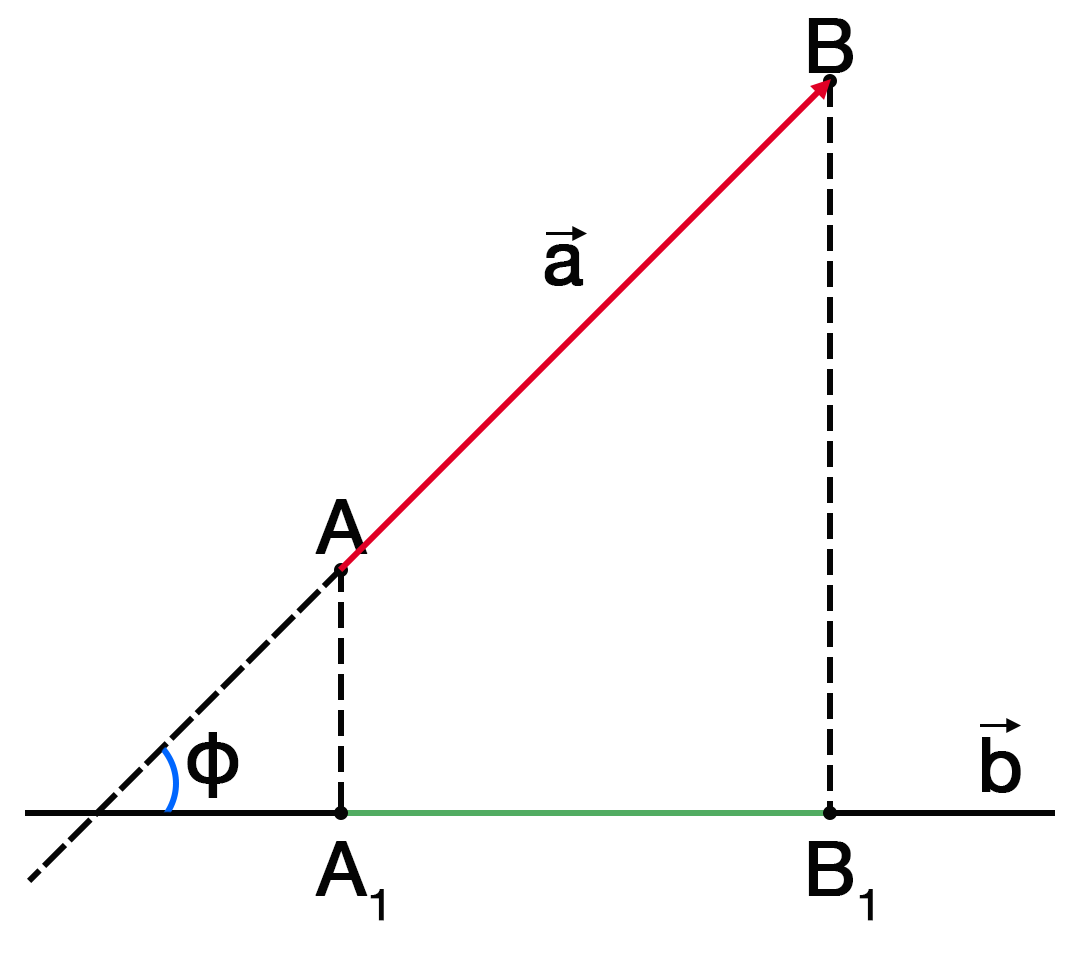
\includegraphics[width=0.5\textwidth]{projection.png}
\end{center}

Проекция вектора \(\vv{AB} = \vv{a}\) обозначается формулой: \(\text{Пр}_{\vv{b}}\vv{AB}\) или \(\text{Пр}_{\vv{b}}\vv{a}\)

Проекция вектора \(\vv{a}\) на ось \(\vv{b}\) выражается формулой:
\begin{gather*}
    \text{Пр}_{\vv{b}}\vv{a} = |\vv{a}| \cdot \cos{\varphi}
\end{gather*}

С другой стороны:
\begin{gather*}
    \cos{\varphi} = \frac{\vv{a} \cdot \vv{b}}{|\vv{a}| \cdot |\vv{b}|}
\end{gather*}

Следовательно:
\begin{gather*}
    \text{Пр}_{\vv{b}}\vv{a} = |\vv{a}| \cdot \cos{\varphi} \iff
    \text{Пр}_{\vv{b}}\vv{a} = \frac{|\vv{a}| \cdot \vv{a} \cdot \vv{b}}{|\vv{a}| \cdot \vv{b}} \iff
    \text{Пр}_{\vv{b}}\vv{a} =
    \frac{\vv{a} \cdot \vv{b}}{|\vv{b}|}
\end{gather*}

\subsection{Свойства проекций}
\begin{enumerate}
    \item {
          \(    \text{Пр}_{\vv{b}}(\vv{a_1} + \vv{a_2} + \vv{a_3}) =
          \text{Пр}_{\vv{b}}\vv{a_1} +
          \text{Пр}_{\vv{b}}\vv{a_2} +
          \text{Пр}_{\vv{b}}\vv{a_3}
          \)
          }
    \item {
          \(
          \text{Пр}_{\vv{b}}(\lambda \cdot \vv{a}) = \lambda \cdot \text{Пр}_{\vv{b}}\vv{a}
          \)
          }
\end{enumerate}

\section{Векторное произведение и его свойства}%
\label{sec:Векторное произведение и его свойства}

\begin{definition}
    Векторным произведением \(\vv{a}\) на \(\vv{b}\) называется \(\vv{c}\), \textbf{длина} которого численно \textbf{равна площади параллелограмма}, построенного на \(\vv{a}\) и \(\vv{b}\), перпендикулярного к плоскости этих векторов и направленного так, чтоб \textbf{наименьшее вращение} от \(\vv{a}\) к \(\vv{b}\) вокруг вектора \(\vv{c}\) осуществлялось \textbf{против часовой} стрелки, если смотреть с конца \(\vv{c}\):

    \begin{center}
        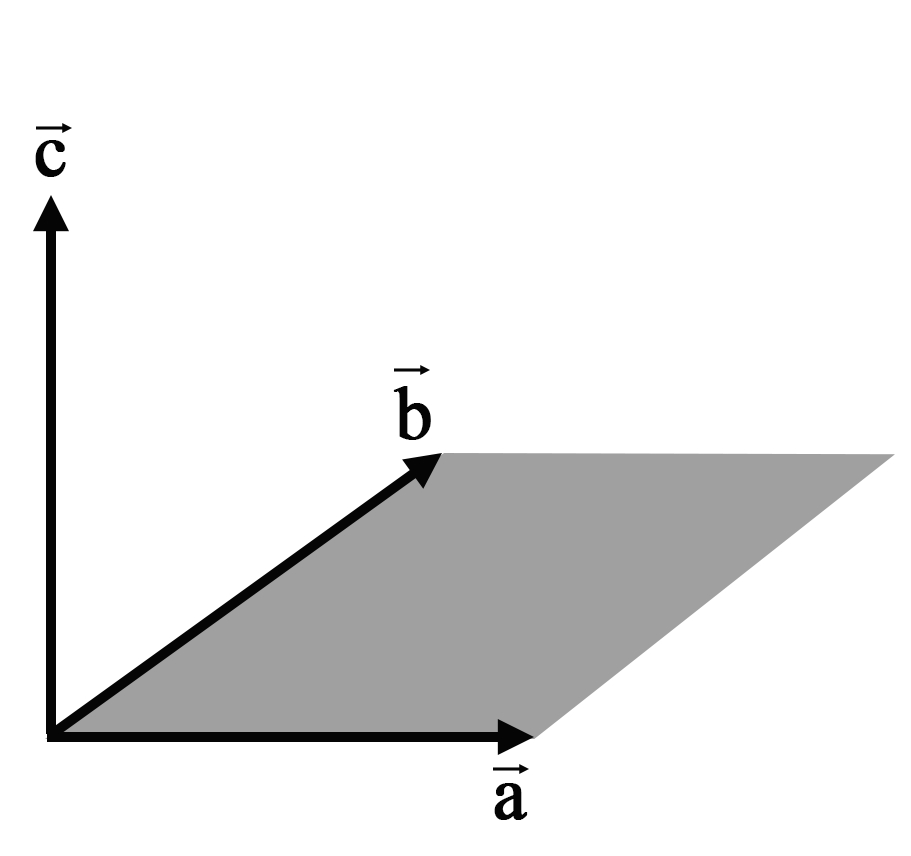
\includegraphics[width=0.4\textwidth]{vector_product.png}
    \end{center}

    Векторное произведение обозначается либо как \(\vv{a} \times \vv{b}\), либо как \([\vv{a}, \vv{b}]\).
\end{definition}

\subsection{Вычисление векторного произведения}%
\label{sub:Вычисление векторного произведения}
Векторное произведение двух векторов \(\vv{a} = (a_x; a_y; a_z)\) и \(\vv{b} = (b_x; b_y; b_z)\) в декартовой системе координат — это \textbf{вектор}, значение которого можно вычислить по формуле:
\[
    \vv{a} \times \vv{b} =
    \begin{vmatrix}
        i   & j   & k   \\
        a_x & a_y & a_z \\
        b_x & b_y & b_z
    \end{vmatrix}
    = (a_y b_z - a_z b_y)\vv{i} - (a_x b_z - a_z b_x)\vv{j} + (a_x b_y - a_y b_x)\vv{k}
\]
\[
    \vv{a} \times \vv{b} = (a_y b_z - a_z b_y, a_z b_x - a_x b_z, a_x b_y - a_y b_x)
\]

\subsection{Геометрический смысл векторного произведения}%
\label{sub:Геометрический смысл векторного произведения}
Модуль векторного произведения двух векторов \(\vv{a}\) и \(\vv{b}\) равен площади параллелограмма, построенного на этих векторах:
\[
    S_{\text{парал-ма}} = |\vv{a} \times \vv{b}|
\]
Как следствие, площадь треугольника, построенного на этих же векторах равна половине модуля векторного произведения:
\[
    S_{\Delta} = \frac{1}{2} |\vv{a} \times \vv{b}|
\]

\subsection{Свойства векторного произведения}%
\label{sub:Свойства векторного произведения}

\begin{enumerate}
    \item {\(\vv{a} \times \vv{b} = - \vv{b} \times \vv{a}\)}

    \item {\((k \vv{a}) \times \vv{b} = \vv{a} \times (k \vv{b}) = k(\vv{a} \times \vv{b})\)}

    \item {\((\vv{a} + \vv{b}) \times \vv{c} = \vv{a} \times \vv{c} + \vv{b} \times \vv{c}\)}

    \item {\(\vv{a} \neq \vv{0}, \vv{b} \neq \vv{0}, \vv{a} \times \vv{b} = 0 \implies \vv{a} || \vv{b}\)}

    \item {\(\vv{a} \neq \vv{0}, \vv{b} \neq \vv{0}, \vv{c} = \vv{a} \times \vv{b} \implies \vv{c} \perp \vv{a}, \vv{c} \perp \vv{b} \)}
\end{enumerate}

\section{Смешанное произведение векторов и его свойства}%
\label{sec:Смешанное произведение векторов и его свойства}

\begin{definition}
    Смешанное произведение векторов — это скалярное произведение вектора \(\vv{a}\) на векторное произведение векторов \(\vv{b}\) и \(\vv{c}\):
    \[
        \vv{a} \cdot (\vv{b} \times \vv{c})
    \]
    Смешанное произведение обозначается либо как \(\vv{a} \cdot (\vv{b} \times \vv{c})\), либо как \((\vv{a}, \vv{b}, \vv{c})\).
\end{definition}

\subsection{Вычисление смешанного произведения}%
\label{sub:Вычисление смешанного произведения}

Пусть даны векторы \(\vv{a} = (a_x, a_y, a_z)\), \(\vv{b} = (b_x, b_y, b_z)\), \(\vv{c} = (c_x, c_y, c_z)\), тогда их смешанное произведение в декартовой системе координат будет равно:
\[
    \vv{a} \cdot (\vv{b} \times \vv{c}) =
    \begin{vmatrix}
        a_x & a_y & a_z \\
        b_x & b_y & b_z \\
        c_x & c_y & c_z
    \end{vmatrix}
\]

\subsection{Геометрический смысл смешанного произведения}%
\label{sub:Геометрический смысл смешанного произведения}
Модуль смешанного произведения векторов \(\vv{a}\), \(\vv{b}\), \(\vv{c}\) равен объему параллелепипеда, образованного этими векторами:
\[
    V_{\text{парал-да}} = |\vv{a} \cdot (\vv{b} \times \vv{c})|
\]

Как следствие, объем пирамиды, образованной на этих же векторах равна одной шестой модуля смешанного произведения:
\[
    V_{\text{пирамиды}} = \frac{1}{6} |\vv{a} \cdot (\vv{b} \times \vv{c})|
\]

\subsection{Алгебраические свойства смешанного произведения}%
\label{sub:Алгебраические свойства смешанного произведения}
\begin{enumerate}
    \item {\(\vv{a} \cdot (\vv{b} \times \vv{c}) = \vv{b} \cdot (\vv{c} \times \vv{a}) = \vv{c} \cdot (\vv{a} \times \vv{b})\)}

    \item {\(\vv{a} \cdot (\vv{b} \times \vv{c}) = - \vv{a} \cdot (\vv{c} \times \vv{b})\)}

    \item {\(\vv{a} \cdot (\vv{b} \times \vv{c}) = (\vv{a} \times \vv{b}) \cdot \vv{c}\)}
\end{enumerate}

\begin{proof}
    \begin{enumerate}
        \item {Длины векторов \(\vv{a}\), \(\vv{b}\), \(\vv{c}\) и ориентация тройки не меняются.}

        \item {Модули слева и справа равны, а ориентация изменилась при перестановке \(\vv{b}\) и \(\vv{c}\) местами.}

        \item {Следует из свойств (1) и (2).}
    \end{enumerate}
\end{proof}

\subsection{Геометрические свойства смешанного произведения}%
\label{sub:Геометрические свойства смешанного произведения}

\begin{theorem}
    \newpar
    Векторы \(\vv{a}\), \(\vv{b}\), \(\vv{c}\) компланарны тогда и только тогда, когда их смешанное произведение равно нулю.
\end{theorem}

\begin{proof}
    Пусть \((\vv{a}, \vv{b}, \vv{c}) = 0\), тогда может быть два случая:

    \textbf{Случай 1.} \(\vv{b} \times \vv{c} = 0 \implies \vv{b} || \vv{c}\)
    \[
        \text{Тогда} \quad \exists k_1, k_2: \vv{c} = k_1 \vv{a} + k_2 \vv{b} \implies \text{коллинеарность — компланарность.}
    \]

    \textbf{Случай 2.} \(\vv{a} \perp (\vv{b} \times \vv{c})\)

    Доказательство следует напрямую из векторного произведения:
    \[
        \vv{a} \perp (\vv{b} \times \vv{c}) \implies \vv{a} \subset \alpha_{(\vv{b}, \vv{c})} \implies \text{векторы компланарны}
    \]

    Верно и обратное:
    \[
        \vv{a}, \vv{b}, \vv{c} \text{ компланарны }, \vv{a} \perp (\vv{b} \times \vv{c}) \implies
        \vv{a} \cdot (\vv{b} \times \vv{c}) = 0.
    \]
\end{proof}

\subsection{Алгебраические свойства смешанного произведения}%
\label{sub:Алгебраические свойства смешанного произведения}
% TODO добавить алгебраические свойства смешанного произведения


\chapter{Определители}%
\label{cha:Определители}


\section{Определители 2-го и 3-го порядка. Разложение определителя по элементам строки}%
\label{sec:Определители 2-го и 3-го порядка}

Пусть дан определитель
\[
    \begin{vmatrix}
        a_{11} & a_{12} & a_{13} \\
        a_{21} & a_{22} & a_{23} \\
        a_{31} & a_{32} & a_{33}
    \end{vmatrix}
\]

Для ускорения вычисления определителя \textbf{третьего порядка} можно воспользоваться \textbf{методом треугольника}.

Вычисление выполняется по следующей схеме:

\begin{center}
    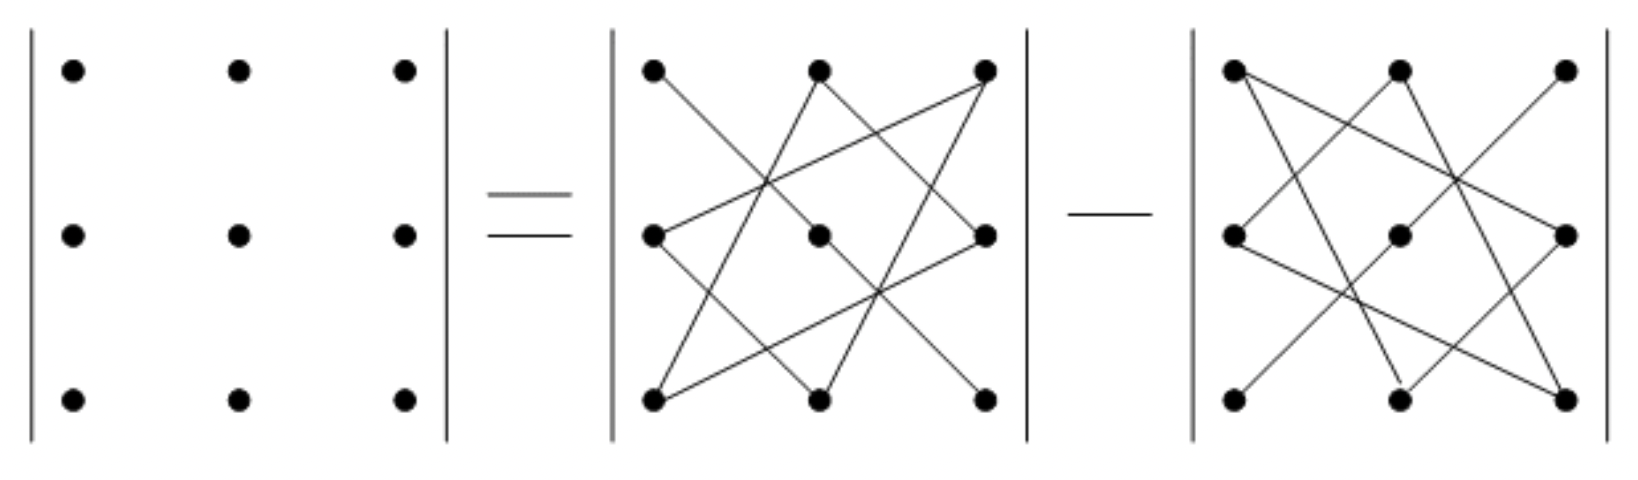
\includegraphics[width=0.65\textwidth]{triangle_rule.png}
\end{center}

Следовательно:

\begin{gather*}
    \begin{vmatrix}
        a_{11} & a_{12} & a_{13} \\
        a_{21} & a_{22} & a_{23} \\
        a_{31} & a_{32} & a_{33}
    \end{vmatrix}
    =                                                                                                      \\
    a_{11} \cdot a_{22} \cdot a_{33} + a_{31} \cdot a_{12} \cdot a_{23} + a_{23} \cdot a_{13} \cdot a_{32} \; - \\
    - \; a_{31} \cdot a_{22} \cdot a_{13} - a_{21} \cdot a_{12} \cdot a_{33} - a_{11} \cdot a_{23} \cdot a_{32}
\end{gather*}

\textbf{Правило Саррюса} — еще один метод вычисления определителя матрицы \textbf{третьего порядка}.
Наряду с правилом треугольника оно призвано внести в процесс вычисления определителя наглядность, уменьшив тем самым вероятность возникновения ошибки.

Действие выполняется согласно следующей схеме:

\begin{center}
    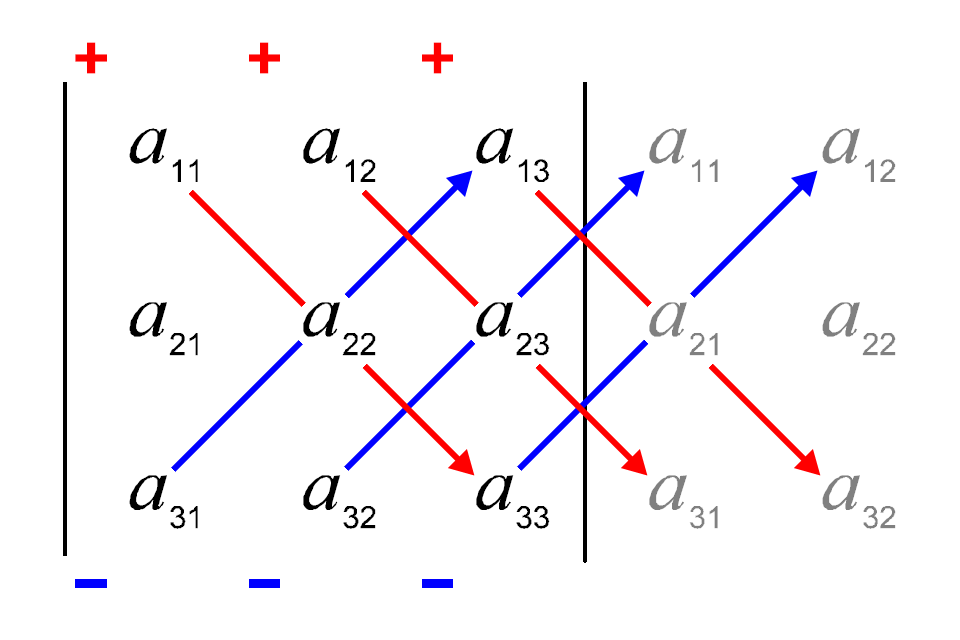
\includegraphics[width=0.35\textwidth]{sarrus_rule.png}
\end{center}

\section{Свойства определителей}%
\label{sec:Свойства определителей}

1. Определитель транспонированной матрицы равен определителю исходной матрицы: \(\det A^T = \det A\)

2. Умножение всех элементов строки или столбца определителя на некоторое число \(\lambda\) равносильно умножению определителя на это число:
\begin{gather*}
    \begin{vmatrix}
        a_{11}         & a_{12}         & \dots a_{1j}         & \dots & a_{1n}         \\
        a_{21}         & a_{22}         & \dots a_{2j}         & \dots & a_{2n}         \\
        \dots          & \dots          & \dots                & \dots & \dots          \\
        \lambda a_{i1} & \lambda a_{i2} & \dots \lambda a_{ij} & \dots & \lambda a_{in} \\
        \dots          & \dots          & \dots                & \dots & \dots          \\
        a_{m1}         & a_{m2}         & \dots a_{mj}         & \dots & a_{mn}         \\
    \end{vmatrix}
    =
    \lambda \cdot
    \begin{vmatrix}
        a_{11} & a_{12} & \dots a_{1j} & \dots & a_{1n} \\
        a_{21} & a_{22} & \dots a_{2j} & \dots & a_{2n} \\
        \dots  & \dots  & \dots        & \dots & \dots  \\
        a_{i1} & a_{i2} & \dots a_{ij} & \dots & a_{in} \\
        \dots  & \dots  & \dots        & \dots & \dots  \\
        a_{m1} & a_{m2} & \dots a_{mj} & \dots & a_{mn} \\
    \end{vmatrix}
\end{gather*}

3. Если в определителе переставить местами любые две строки или два столбца, то определитель изменяет свой знак на противоположный:
\begin{gather*}
    \begin{vmatrix}
        \dots  & \dots  & \dots  & \dots & \dots  \\
        a_{i1} & a_{i2} & a_{i3} & \dots & a_{in} \\
        \dots  & \dots  & \dots  & \dots & \dots  \\
        a_{k1} & a_{k2} & a_{k3} & \dots & a_{kn} \\
        \dots  & \dots  & \dots  & \dots & \dots  \\
    \end{vmatrix}
    =
    -
    \begin{vmatrix}
        \dots  & \dots  & \dots  & \dots & \dots  \\
        a_{k1} & a_{k2} & a_{k3} & \dots & a_{kn} \\
        \dots  & \dots  & \dots  & \dots & \dots  \\
        a_{i1} & a_{i2} & a_{i3} & \dots & a_{in} \\
        \dots  & \dots  & \dots  & \dots & \dots  \\
    \end{vmatrix}
\end{gather*}

4. Если матрица содержит нулевую строку (столбец), то определитель этой матрицы равен нулю:
\begin{gather*}
    \begin{vmatrix}
        \dots  & \dots  & \dots  & \dots & \dots  \\
        a_{i1} & a_{i2} & a_{i3} & \dots & a_{in} \\
        0      & 0      & 0      & \dots & 0      \\
        a_{j1} & a_{j2} & a_{j3} & \dots & a_{jn} \\
        \dots  & \dots  & \dots  & \dots & \dots  \\
    \end{vmatrix}
    = 0
\end{gather*}

5. Если две строки (столбца) матрицы равны между собой, то определитель этой матрицы равен нулю:
\begin{gather*}
    \begin{vmatrix}
        \dots  & \dots  & \dots  & \dots & \dots  \\
        a_{i1} & a_{i2} & a_{i3} & \dots & a_{in} \\
        \dots  & \dots  & \dots  & \dots & \dots  \\
        a_{i1} & a_{i2} & a_{i3} & \dots & a_{in} \\
        \dots  & \dots  & \dots  & \dots & \dots  \\
    \end{vmatrix}
    = 0
\end{gather*}

6. Если две строки (столбца) матрицы пропорциональны друг другу, то определитель этой матрицы равен нулю:
\begin{gather*}
    \begin{vmatrix}
        \dots   & \dots   & \dots   & \dots & \dots   \\
        a_{i1}  & a_{i2}  & a_{i3}  & \dots & a_{in}  \\
        \dots   & \dots   & \dots   & \dots & \dots   \\
        ca_{i1} & ca_{i2} & ca_{i3} & \dots & ca_{in} \\
        \dots   & \dots   & \dots   & \dots & \dots   \\
    \end{vmatrix}
    = 0
\end{gather*}

7. Определитель матрицы треугольного вида равен произведению элементов, стоящих на главной диагонали:
\begin{gather*}
    \begin{vmatrix}
        a_{11} & a_{12} & a_{13} & \dots & a_{1n} \\
        0      & a_{22} & a_{23} & \dots & a_{2n} \\
        0      & 0      & a_{33} & \dots & a_{3n} \\
        \dots  & \dots  & \dots  & \dots & \dots  \\
        0      & 0      & 0      & \dots & a_{mn} \\
    \end{vmatrix}
    = a_{11} \cdot a_{22} \cdot a_{33} \cdot ... \cdot a_{mn}
\end{gather*}

8. Если все элементы k-ой строки (столбца) определителя представлены в виде сумм \(a_{kj} + b_{kj}\), то определитель можно представить в виде суммы соответствующих определителей:
\begin{gather*}
    \hspace{0.9cm}
    \begin{vmatrix}
        a_{11}          & a_{12}          & a_{13}          & \dots & a_{1n}          \\
        \dots           & \dots           & \dots           & \dots & \dots           \\
        a_{k1} + b_{k1} & a_{k2} + b_{k2} & a_{k3} + b_{k3} & \dots & a_{kn} + b_{kn} \\
        \dots           & \dots           & \dots           & \dots & \dots           \\
        a_{m1}          & a_{m2}          & a_{m3}          & \dots & a_{mn}          \\
    \end{vmatrix}
    =
    \\
    =
    \begin{vmatrix}
        a_{11} & a_{12} & a_{13} & \dots & a_{1n} \\
        \dots  & \dots  & \dots  & \dots & \dots  \\
        a_{k1} & a_{k2} & a_{k3} & \dots & a_{kn} \\
        \dots  & \dots  & \dots  & \dots & \dots  \\
        a_{m1} & a_{m2} & a_{m3} & \dots & a_{mn} \\
    \end{vmatrix}
    +
    \begin{vmatrix}
        a_{11} & a_{12} & a_{13} & \dots & a_{1n} \\
        \dots  & \dots  & \dots  & \dots & \dots  \\
        b_{k1} & b_{k2} & b_{k3} & \dots & b_{kn} \\
        \dots  & \dots  & \dots  & \dots & \dots  \\
        a_{m1} & a_{m2} & a_{m3} & \dots & a_{mn} \\
    \end{vmatrix}
\end{gather*}

9. Определитель не изменится, если к элементам любой его строки (или столбца) прибавить соответствующие элементы другой строки (или соответствующего столбца), умноженные на одно и тоже число:
\begin{gather*}
    \begin{vmatrix}
        \dots  & \dots  & \dots  & \dots & \dots  \\
        a_{i1} & a_{i2} & a_{i3} & \dots & a_{in} \\
        \dots  & \dots  & \dots  & \dots & \dots  \\
        a_{k1} & a_{k2} & a_{k3} & \dots & a_{kn} \\
        \dots  & \dots  & \dots  & \dots & \dots  \\
    \end{vmatrix}
    =
    \begin{vmatrix}
        \dots            & \dots            & \dots            & \dots & \dots            \\
        a_{i1}           & a_{i2}           & a_{i3}           & \dots & a_{in}           \\
        \dots            & \dots            & \dots            & \dots & \dots            \\
        a_{k1} + ca_{i1} & a_{k2} + ca_{i2} & a_{k3} + ca_{i3} & \dots & a_{kn} + ca_{in} \\
        \dots            & \dots            & \dots            & \dots & \dots            \\
    \end{vmatrix}
\end{gather*}

10. Пусть A и B – квадратные матрицы одного и того же порядка. Тогда определитель произведения матриц равен произведению определителей:
\begin{gather*}
    \det (AB) = \det A \cdot \det B
\end{gather*}

\section{Теорема Крамера}%
\label{sec:Теорема Крамера}

\textbf{Метод крамера} (правило Крамера) — способ решения систем линейных алгебраических уравнений с \textbf{числом уравнений равным числу неизвестных} с \underline{ненулевым} главным определителем матрицы коэффициентов системы (причём для таких уравнений решение существует и единственно).

\begin{theorem*}[Крамера]
    \newpar
    Для системы линейных уравнения вида:

    \begin{gather*}
        \begin{cases}
            \begin{matrix}
                a_{11}x_1 & +      & a_{12}x_2 & +      & \cdots & +      & a_{1n}x_n & =      & b_1    \\
                a_{21}x_1 & +      & a_{22}x_2 & +      & \cdots & +      & a_{2n}x_n & =      & b_2    \\
                \cdots    & \cdots & \cdots    & \cdots & \cdots & \cdots & \cdots    & \cdots & \cdots \\
                a_{n1}x_1 & +      & a_{n2}x_2 & +      & \cdots & +      & a_{nn}x_n & =      & b_n
            \end{matrix}
        \end{cases}
    \end{gather*}

    Матрица коэффициентов:

    \begin{equation*}
        A = \left(
        \begin{array}{cccc}
            a_{11} & a_{12} & \cdots & a_{1n} \\
            a_{21} & a_{22} & \cdots & a_{2n} \\
            \cdots & \cdots & \cdots & \cdots \\
            a_{n1} & a_{n2} & \cdots & a_{nn}
        \end{array}
        \right)
    \end{equation*}

    Матрица правых частей:

    \begin{equation*}
        B = \left(
        \begin{array}{cccc}
            b_{1}  \\
            b_{2}  \\
            \cdots \\
            b_{n}
        \end{array}
        \right)
    \end{equation*}

    Справедливо утверждение:

    \begin{equation*}
        x_k = \frac{\det C_k}{\det A} \text{ где } k = 1, 2, \dots, n.
    \end{equation*}

    \(C_k\) — матрица, получаемая заменой \(k\)-го столбца матрицы \(A\) столбцом \(B\).
\end{theorem*}

\begin{proof}

    Рассмотрим систему уравнений:

    \begin{gather*}
        \begin{cases}
            a_{11}x_1 + a_{12}x_2 = b_1 \\
            a_{21}x_1 + a_{22}x_2 = b_2
        \end{cases}
    \end{gather*}

    Тогда:

    \begin{gather*}
        \begin{cases}
            x_1 = \dfrac{a_{11}b_1 - a_{12}b_1}{a_{11}a_{22} - a_{21}a_{12}} = \dfrac{\Delta{x_1}}{\Delta}
            \vspace{0.5cm} \\
            x_2 = \dfrac{a_{11}b_2 - a_{21}b_1}{a_{11}a_{22} - a_{21}a_{12}} = \dfrac{\Delta{x_2}}{\Delta}
        \end{cases}
    \end{gather*}

    где:

    \begin{equation*}
        \Delta =
        \begin{vmatrix}
            a_{11} & a_{12} \\
            a_{21} & a_{22}
        \end{vmatrix}
        \qquad
        \Delta{x_1} =
        \begin{vmatrix}
            b_{1} & a_{12} \\
            b_{2} & a_{22}
        \end{vmatrix}
        \qquad
        \Delta{x_2} =
        \begin{vmatrix}
            a_{11} & b_{1} \\
            a_{21} & b_{2}
        \end{vmatrix}
    \end{equation*}
\end{proof}

\chapter{Прямые и плоскости}%
\label{cha:Прямые и плоскости}

\section{Системы координат. преобразования сдвига и поворота}
\label{sec:coordinate_systems}

\subsection{Декартова система координат}

Расположение точки \(P\) на плоскости определяется декартовыми координатами с помощью пары чисел \((x, y)\):
\begin{itemize}
    \item {x — расстояоние от точки \(P\) до оси \(y\) с учетом знака}
    \item {y — расстояоние от точки \(P\) до оси \(x\) с учетом знака}
\end{itemize}

\begin{center}
    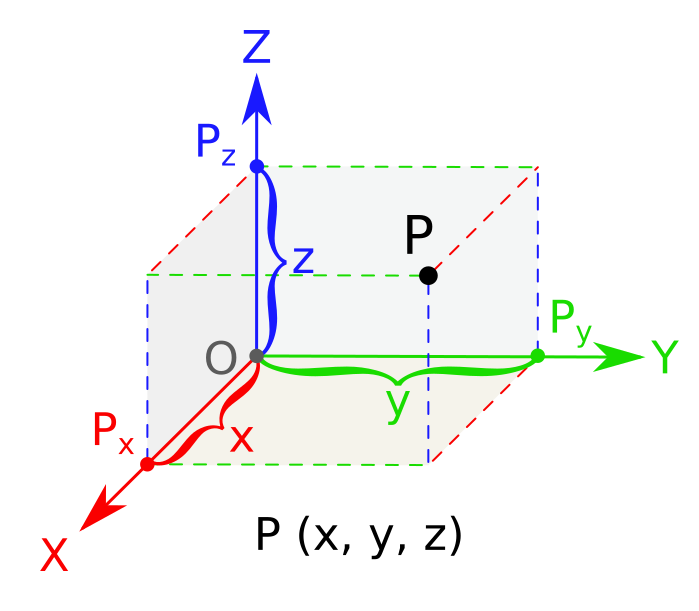
\includegraphics[width=0.6\textwidth]{cartesian_system.png}
\end{center}

В пространстве уже необходимы три координаты \((x, y, z)\) :
\begin{itemize}
    \item {x — расстояоние от точки \(P\) до плоскости \(yz\)}
    \item {y — расстояоние от точки \(P\) до плоскости \(xz\)}
    \item {z — расстояоние от точки \(P\) до плоскости \(xy\)}
\end{itemize}

\subsection{Полярная система координат}
Полярная система координат задаётся лучом, который называют \textbf{нулевым лучом} или \textbf{полярной осью}.
В нашем случае полярная ось совпадает с осью \(Ox\).
Точка, из которой выходит этот луч, называется \textbf{началом координат} или \textbf{полюсом}.
На схеме таковой точкой является точка \(O\).

Пусть \(M (r, \varphi)\) — произвольная точка в полярной системе координат.
Положение точки \(M\) фиксируется двумя числами: \textbf{радиусом} \(r = \vv{OM}\) и углом \(\varphi\) между полярной осью и вектором \(\vv{OM}\).
Этот угол называется \textbf{полярным углом}.

\begin{center}
    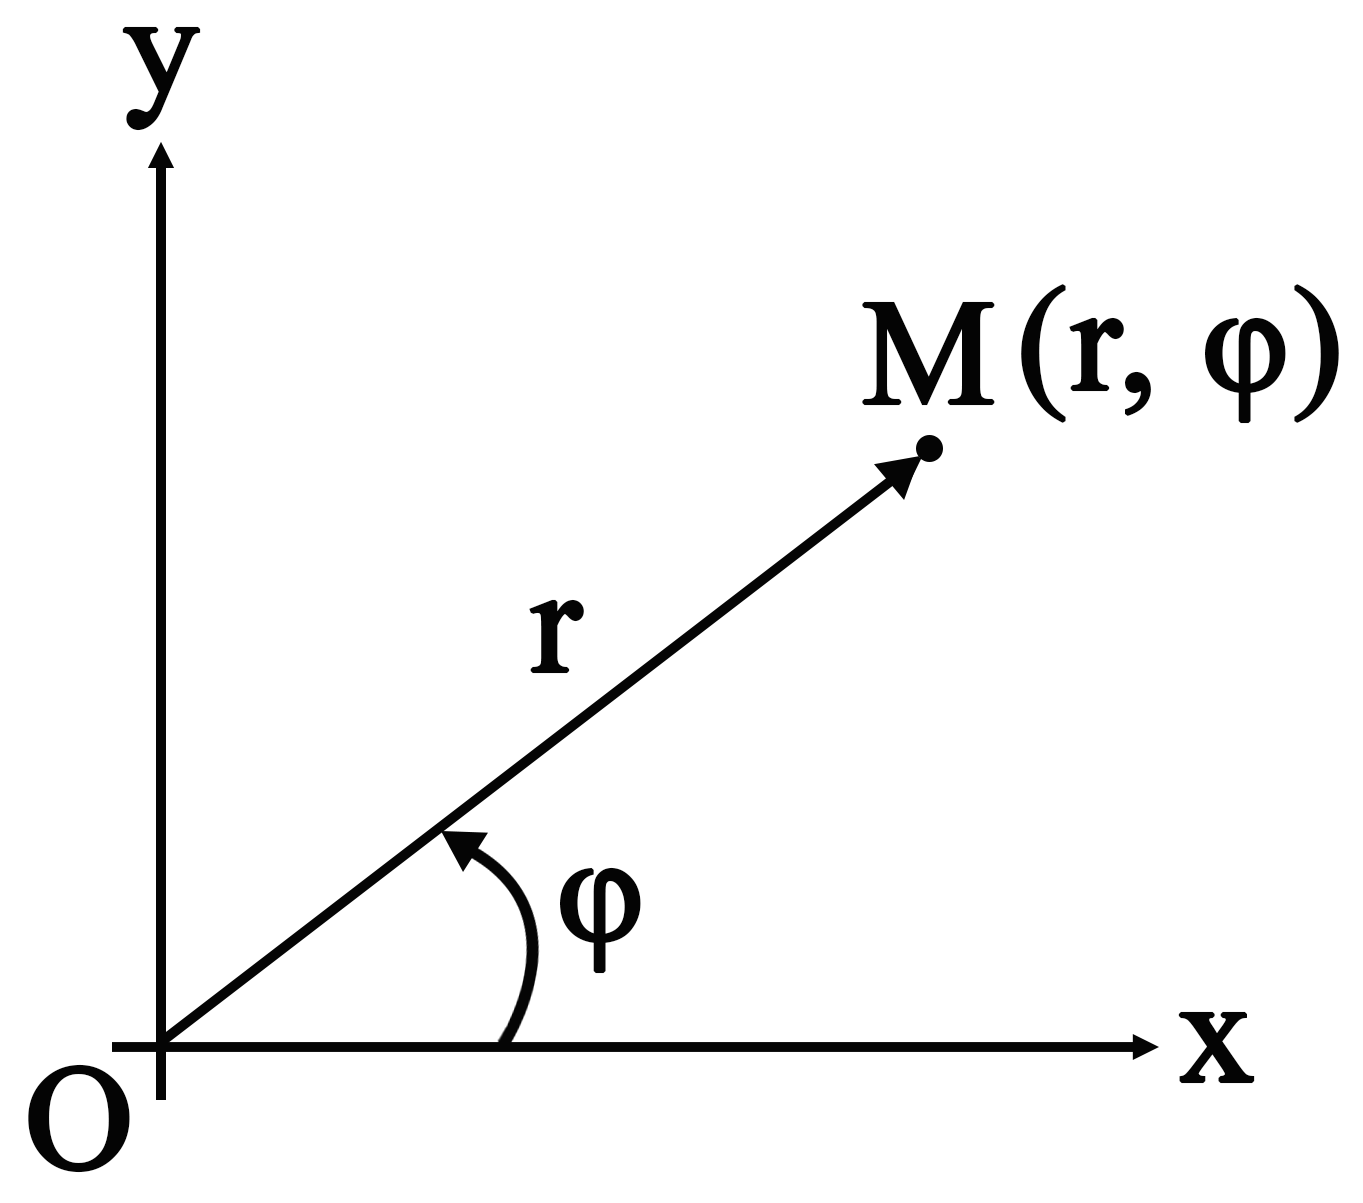
\includegraphics[width=0.5\textwidth]{polar_system.png}
\end{center}

Декартовы координаты точки выражаются формулами:
\begin{gather*}
    x = r \cos{\varphi} \\
    y = r \sin{\varphi}
\end{gather*}

\subsubsection{Обозначения и ограничения}
\begin{itemize}
    \item {\(r \geq 0\) — радиус (также обозначают за \(r\))}
    \item {\(0 \leq \varphi < 2\pi\) или \(-\pi < \varphi \leq \pi\) — азимут или долгота (также обозначают за \(\theta\))}
\end{itemize}

Полярный радиус определен для любой точки плоскости и всегда принимает неотрицательные значения \(r \geq 0\).

Полярный угол \(\varphi\) определен для любой точки плоскости, за исключением полюса \(O\), и принимает значения \(-\pi < \varphi \leq \pi\), то есть координаты \((r, \varphi + 2\pi)\) и  \((r, \varphi + 4\pi)\) соответствуют одной точке.
Полярный угол отсчитывается от полярной оси против часовой стрелки и измеряется в радианах.

\subsubsection{Достоинства}
Полярная система координат особенно полезна в случаях, когда отношения между точками проще изобразить в виде радиусов и углов; в более распространённой декартовой, или прямоугольной, системе координат, такие отношения можно установить только путём применения тригонометрических уравнений.

\subsubsection{Недостатки}
\begin{itemize}
    \item Угол \(\varphi\) не определен, если \(r = 0\).
\end{itemize}

\subsection{Цилиндрическая система координат}
Цилиндрические координаты — трёхмерный аналог полярных координат,
являющуюся расширением полярной системы координат путём добавления третьей координаты (обычно обозначаемой \(h\) или \(z\)), которая задаёт высоту точки над плоскостью.

\begin{center}
    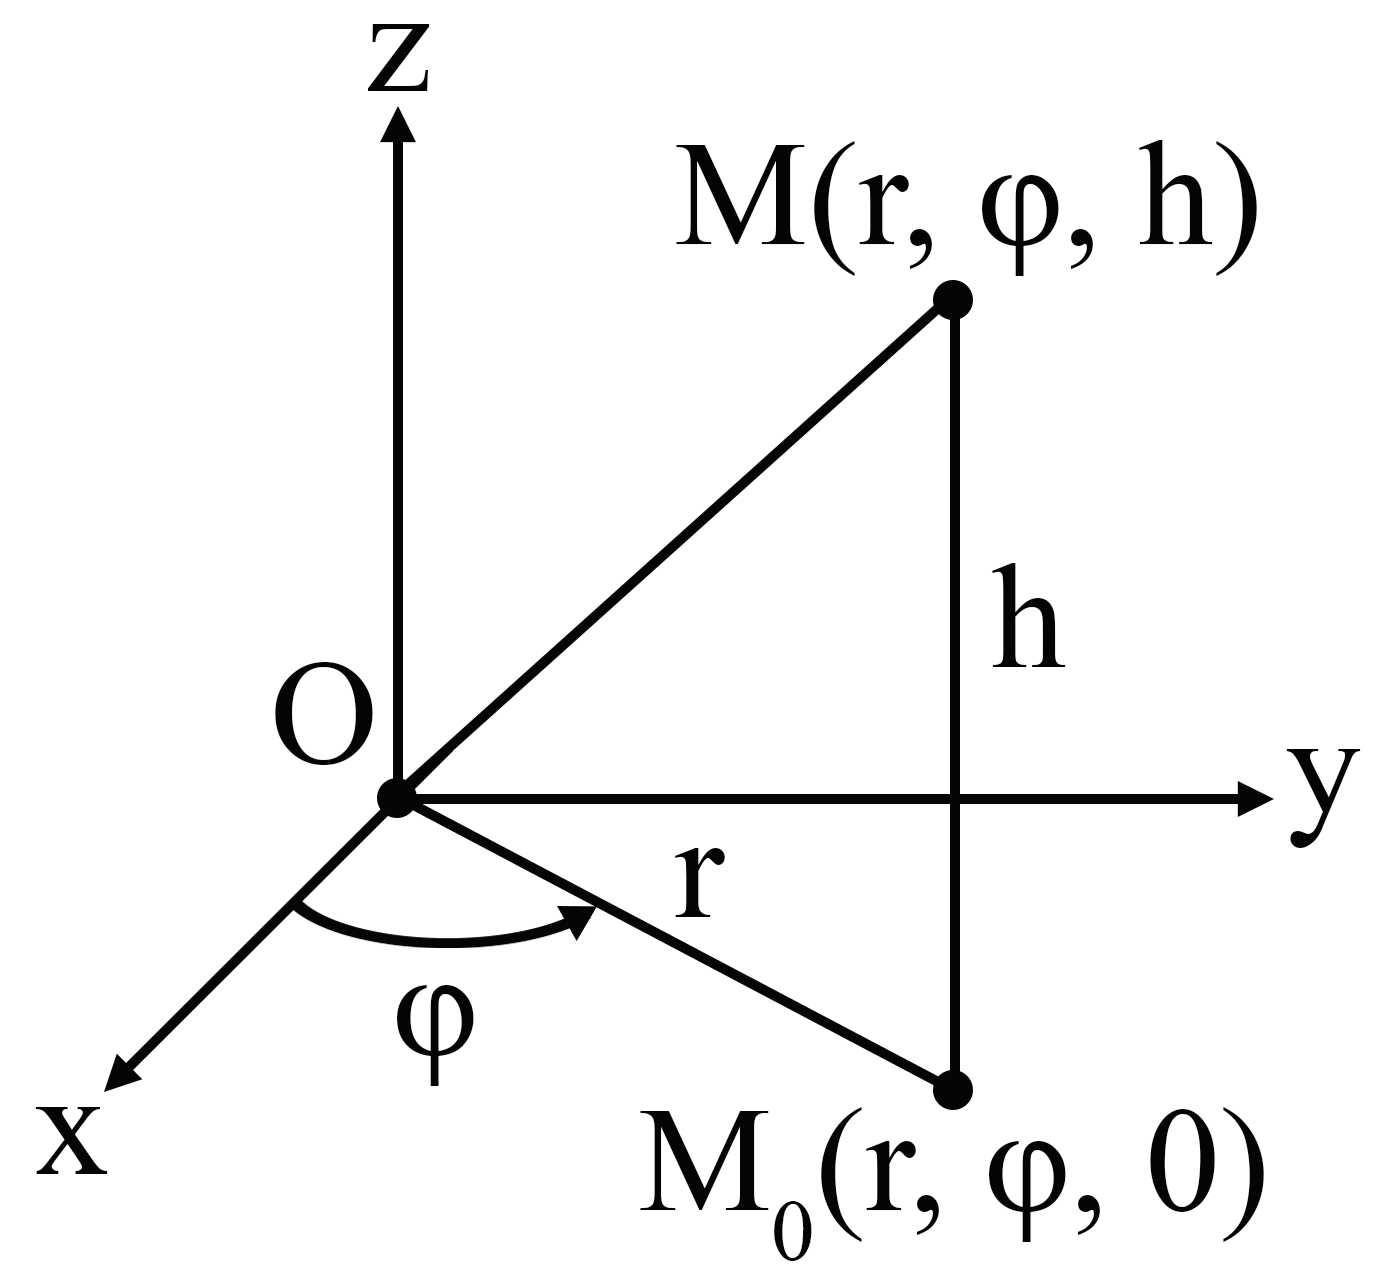
\includegraphics[width=0.5\textwidth]{cylindrical_system.png}
\end{center}

Пусть \(M(r, \varphi, h)\) — произвольная точка циллиндрической системы координат, а \(M_0(r, \varphi, 0)\) — ее проекция на плоскость \(xy\). Тогда:
\begin{itemize}
    \item[]{\(r\) — это расстояние от точки \(M\) до оси \(Oz\)}
    \item[]{\(\varphi\) — угол между осью \(Ox\) и отрезком \(OM_0\)}
    \item[]{\(h\) — расстояние от точки \(M\) до плоскости \(xy\)}
\end{itemize}

\subsubsection{Обозначения и ограничения}
\begin{itemize}
    \item {\(r \geq 0\) — радиус (также обозначают за \(r\))}
    \item {\(0 \leq \varphi < 2\pi\) или \(-\pi < \varphi \leq \pi\) — азимут или долгота (также обозначают за \(\theta\))}
    \item {\(h\) — высота (также обозначают за \(z\))}
\end{itemize}

\subsubsection{Достоинства}
Цилиндрические координаты полезны для изучения систем, симметричных относительно некоторой оси. Например, длинный цилиндр с радиусом R в декартовых координатах (с осью z, совпадающей с осью цилиндра) имеет уравнение \(x^2 + y^2 = R^2\), тогда как в цилиндрических координатах оно выглядит гораздо проще, как \(r = R\).

\subsubsection{Недостатки}
\begin{itemize}
    \item Угол \(\varphi\) не определен, если \(r = 0\).
\end{itemize}

\subsection{Сферическая система координат}
Сферическая система координат — трёхмерная система координат, в которой каждая точка пространства определяется тремя числами \((r, \varphi, \theta)\).

Пусть \(M(r, \varphi, \theta)\) — произвольная точка сферической системы координат, а \(M_0(r, \varphi, 0)\) — ее проекция на плоскость \(xy\). Тогда:
\begin{itemize}
    \item[]{\(r\) — это расстояние от точки \(M\) до полюса \(O\)}
    \item[]{\(\varphi\) — угол между осью \(Ox\) и отрезком \(OM_0\)}
    \item[]{\(\theta\) — угол между осью \(Oz\) и отрезком \(OM\)}
\end{itemize}

\begin{center}
    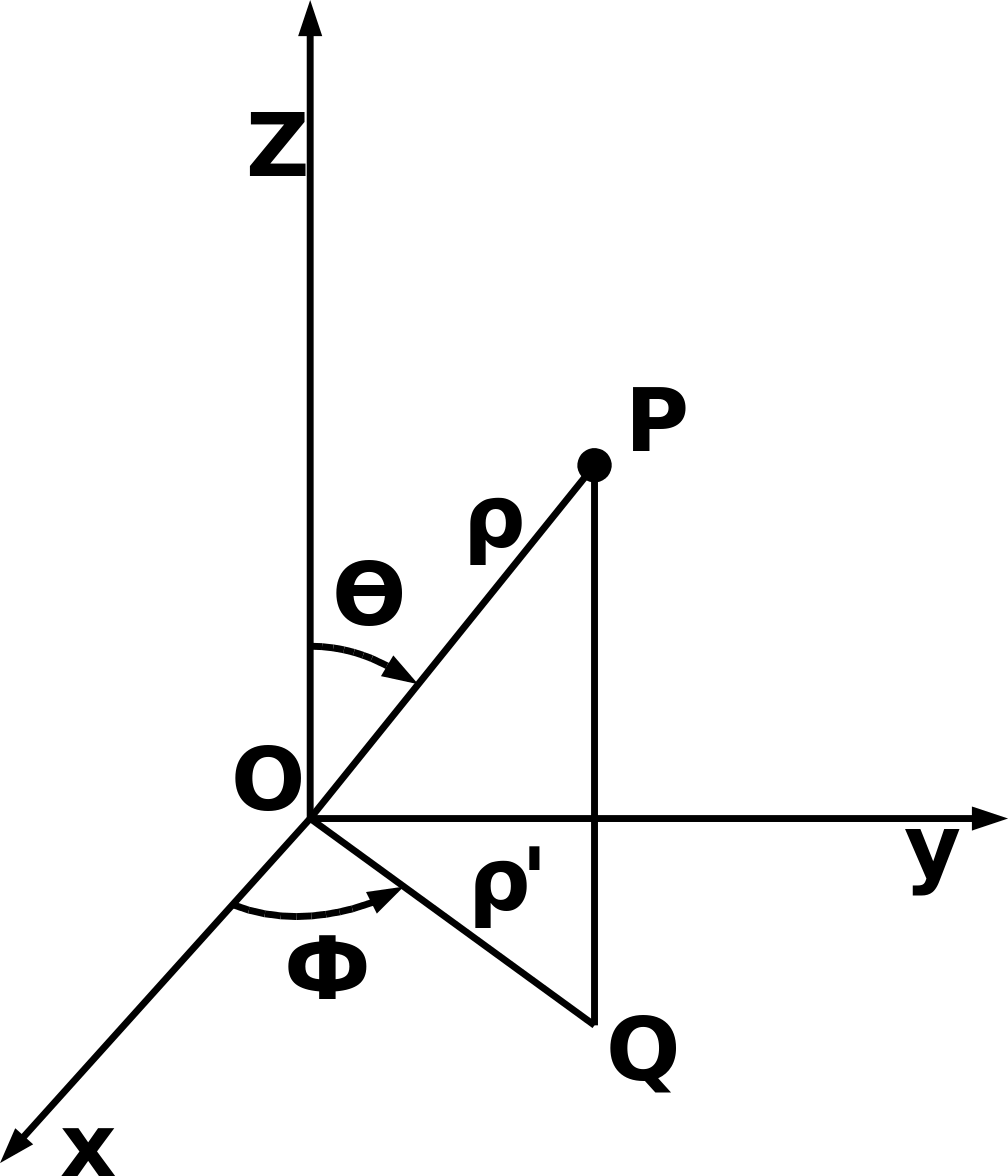
\includegraphics[width=0.5\textwidth]{spherical_system.png}
\end{center}

\subsubsection{Обозначения и ограничения}
\begin{itemize}
    \item {\(r \geq 0\) — радиус (также обозначают за \(r\))}
    \item {\(0 \leq \varphi < 2\pi\) или \(-\pi < \varphi \leq \pi\) — азимут или долгота (также обозначают за \(\theta\))}
    \item {\(0 \leq \theta \leq \pi\) или \(-\dfrac{\pi}{2} \leq \theta \leq \dfrac{\pi}{2}\) — широта или полярный угол (также обозначают за \(\varphi\))}
\end{itemize}

\subsubsection{Достоинства}
Сферические координаты полезны при изучении систем, симметричных относительно точки. Так, уравнение сферы с радиусом R в декартовых координатах с началом отсчёта в центре сферы выглядит как \(x^2 + y^2 = R^2\), тогда как в сферических координатах оно становится намного проще: \(r = R\).

\subsubsection{Недостатки}
\begin{itemize}
    \item Углы \(\varphi\) и \(\theta\) не определены, если \(r = 0\).
    \item Угол \(\varphi\) неопределен для граничных значений \(\theta = 0\) и \(\theta = \pi\) (или для \(\theta = \pm \dfrac{\pi}{2}\), при \(-\dfrac{\pi}{2} \leq \theta \leq \dfrac{\pi}{2}\))
\end{itemize}

\section{Плоскость и ее уравнения}\label{sec:plane}

\textbf{Плоскость} – это геометрическая фигура, состоящая из отдельных точек. Каждой точке в трехмерном пространстве соответствуют координаты, которые задаются тремя числами. Уравнение плоскости устанавливает зависимость между координатами всех точек.

\subsection{Общее уравнение плоскости}
\begin{gather*}
    Ax + By + Cz + D = 0
\end{gather*}
\subsubsection{Теорема}
Всякая плоскость в прямоугольной системе координат \(Oxyz\) в трехмерном пространстве может быть задана уравнением вида \(Ax + By + Cz + D = 0\), где \(A, B, C, D\) — некоторые действительные числа, одновременно не равные нулю. Всякое уравнение, имеющее вид \(Ax + By + Cz + D = 0\) определяет плоскость в трехмерном пространстве.

% TODO добавить доказательство

\subsection{Уравнение плоскости в отрезках}
Если плоскость пересекает оси \(OX\), \(OY\), \(OZ\) в точках с координатами \((a, 0, 0)\), \((0, b, 0)\), \((0, 0, c)\), то она может быть найдена по формуле \textbf{уравнения плоскости в отрезках}:
\begin{gather*}
    \frac{x}{a} + \frac{y}{b} + \frac{z}{c} = 1
\end{gather*}

% TODO добавить доказательство

\subsection{Уравнение плоскости, проходящей через точку, перпендикулярно вектору нормали}
Пусть у нас есть точка \(M(x_0, y_0, z_0)\), принадлежащая плоскости, и вектор нормали плоскости \(\vv{n} = (A, B, C)\). Тогда плоскость задается уравнением:
\begin{gather*}
    A(x - x_0) + B(y - y_0) + C(z - z_0) = 0
\end{gather*}

% TODO добавить доказательство

\subsection{Уравнение плоскости, проходящей через три заданные точки, не лежащие на одной прямой}
Пусть у нас есть три точки \(A(x_1, y_1, z_1)\), \(B(x_2, y_2, z_2)\), \(C(x_3, y_3, z_3)\), лежащих на плоскости и не лежащих на одной прямой. Тогда уравнение плоскости можно найти по формуле:
\begin{gather*}
    \begin{vmatrix}
        x - x_1   & y - y_1   & z - z_1   \\
        x_2 - x_1 & y_2 - y_1 & z_2 - z_1 \\
        x_3 - x_1 & y_3 - y_1 & z_3 - z_1
    \end{vmatrix}
\end{gather*}

% TODO добавить доказательство

\section{Прямая в пространстве и ее уравнения}\label{sec:line_in_space}
Уравнение прямой на плоскости в прямоугольной системе координат \(Oxy\) – это линейное уравнение с переменными \(x\) и \(y\), которому отвечают координаты всех точек прямой и не удовлетворяют координаты никаких прочих точек.

\subsection{Уравнение прямой в пространстве как уравнение двух пересекающихся плоскостей}
Когда две плоскости в пространстве имеют общую точку, существует их общая прямая, на которой находятся все общие точки этих плоскостей.

Пусть у нас есть две плоскости \(\alpha\) и \(\beta\), которые описываются следующими уравнениями плоскости:
\begin{gather*}
    \alpha: A_1x + B_1y + C_1z + D_1 = 0 \\
    \beta: A_2x + B_2y + C_2z + D_2 = 0
\end{gather*}

Прямую их пересечения обозначим за \(l\). Поскольку любая точка прямой удовлетворяет сразу двум уравнениям плоскостей, координаты любой точки прямой будут частным решением системы:
\begin{gather*}
    \begin{cases}
        A_1x + B_1y + C_1z + D_1 = 0 \\
        A_2x + B_2y + C_2z + D_2 = 0
    \end{cases}
\end{gather*}

\subsection{Канонические уравнения прямой в пространстве}
Пусть у нас есть некоторая прямая \(l\), точка \(M_0(x_0, y_0, z_0)\), лежащая на прямой \(l\) и направляющий вектор \(\vv{r} = (m, n, p)\). Пусть \(M(x, y, z)\) — произвольная точка \(l\), тогда вектор \(\vv{M_0M} = (x - x_0, y - y_0, z - z_0)\) и вектор \(r\) коллинеарны. Из условия коллинеарности следует, что:
\begin{gather*}
    \frac{x - x_0}{n} = \frac{y - y_0}{m} = \frac{z - z_0}{p}
\end{gather*}

что является каноническим уравнением прямой в пространстве.

\subsection{Параметрические уравнения прямой в пространстве}
Воспользуется каноническим уравнением прямой, прировняв каждую из дробей к некоторому параметру \(t\):
\begin{gather*}
    \frac{x - x_0}{n} = \frac{y - y_0}{m} = \frac{z - z_0}{p} = t
\end{gather*}
Тогда получим параметрическое уравнение прямой:
\begin{gather*}
    \begin{cases}
        x = x_0 + nt \\
        y = y_0 + mt \\
        z = z_0 + pt
    \end{cases}
\end{gather*}

\subsection{Уравнение прямой через две заданные точки}
Пусть даны две точки \(M_1(x_1, y_1, z_1)\) и \(M_2(x_2, y_2, z_2)\), которые лежат на некоторой прямой \(l\). Тогда вектор  \(\vv{M_1M_2} = (x_2 - x_1, y_2 - y_1, z_2 - z_1)\) явлется направляющим вектором этой прямой.

Пусть у нас есть произвольная точка \(M(x, y, z)\), лежащая на прямой \(l\). Тогда вектор \(\vv{M_1M} = (x - x_1, y - y_1, z - z_1)\) будет коллинеарен вектору \(\vv{M_1M_2}\). Из условия коллинеарности следует, что:
\begin{gather*}
    \frac{x - x_1}{x_2 - x_1} = \frac{y - y_1}{y_2 - y_1} = \frac{z - z_1}{z_2 - z_1}
\end{gather*}

что является уравнением прямой в пространстве, которая проходит через две заданные точки.

\section{Прямая на плоскости: уравнение через две точки, каноническое, параметрическое, общее, в отрезках на осях}\label{sec:line_on_plane}

\subsection{Каноническое уравнение прямой}

Дана прямая \(L\), проходящая через точку \(M_0(x_0;y_0)\), и направляющий вектор \(\vv{a}(m, n)\) этой прямой.
Пусть \(M(x, y)\) — произвольная точка на искомой прямой \(L\), тогда \(M \in L \iff \vv{M_0M} || \vv{a}\).

\begin{center}
    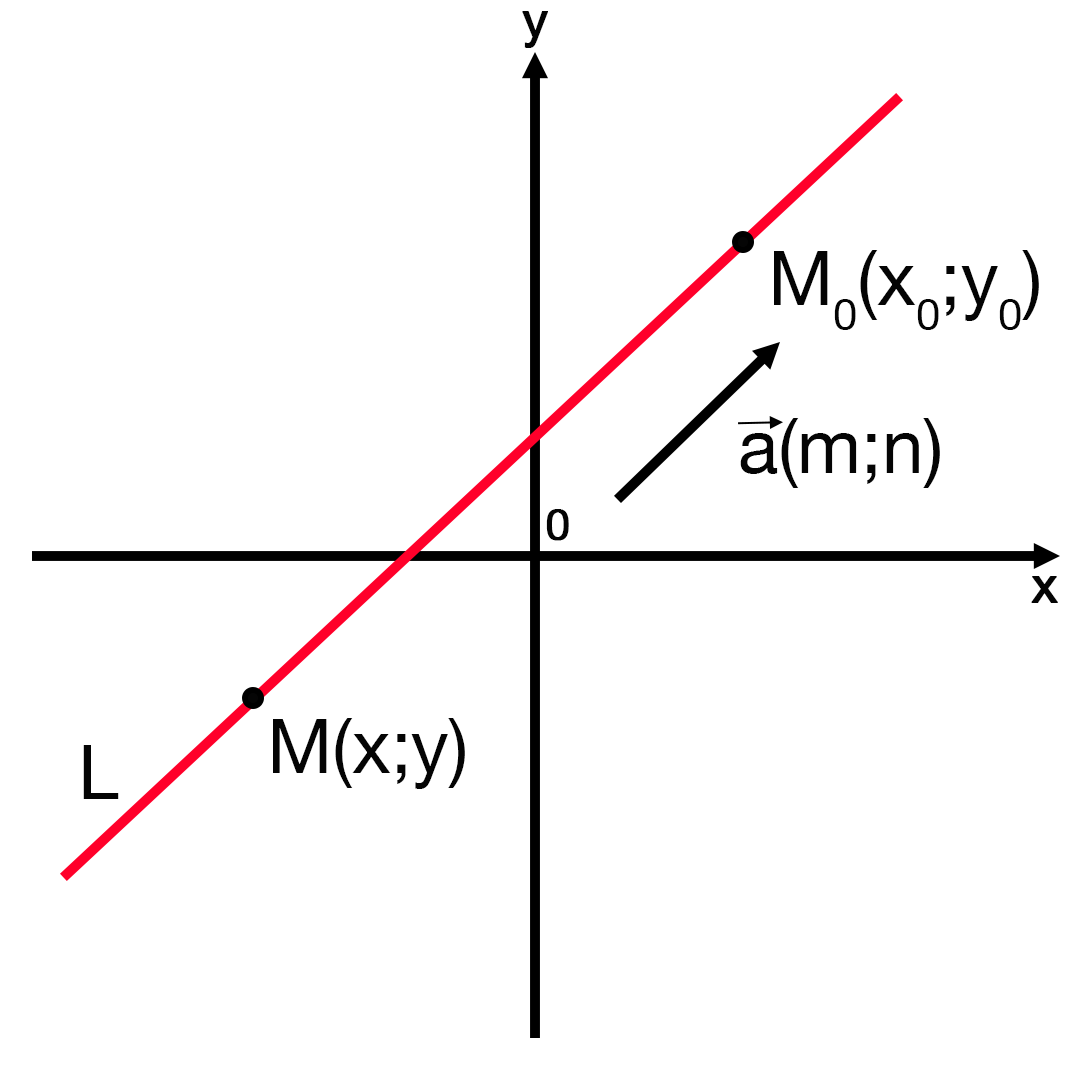
\includegraphics[width=0.5\textwidth]{kanon_line.png}
\end{center}

Условием коллинеарности векторов \(\vv{M_0M}\) и \(\vv{a}\) будет:
\(\dfrac{x - x_0}{m} = \dfrac{y - y_0}{n}\), что и является каноническим уравнением прямой.

\subsection{Уравнение прямой через 2 заданные точки}

Даны две точки \(M_0(x_0;y_0)\) и \(M_1(x_1;y_1)\), лежащие на прямой \(L\).
Из этого следует, что \(\vv{M_0M_1} = (x_1 - x_0; y_1 - y_0)\) — направляющий вектор прямой \(L\).

Тогда искомое уравнение будет иметь вид: \(\dfrac{x - x_0}{x_1 - x_0} = \dfrac{y - y_0}{y_1 - y_0}\).

\subsection{Параметрическое уравнение прямой}

Уравнение \(\vv{M_0M} = \lambda \cdot \vv{a}\) называют векторно-параметрическим уравнением прямой, где \lambda — некоторое действительное число.

В векторной форме оно имеет вид:
\begin{gather*}
    \vv{M_0M} = \lambda \cdot \vv{a} \iff
    \begin{cases}
        x - x_0 = \lambda \cdot m \\
        y - y_0 = \lambda \cdot n
    \end{cases}
    \iff
    \begin{cases}
        x = x_0 + \lambda \cdot m \\
        y = y_0 + \lambda \cdot n
    \end{cases}
\end{gather*}

\subsection{Общее уравнение прямой}

Уравнение, имеющее вид \(Ax + By + C = 0\) — это общее уравнение прямой на плоскости в прямоугольной системе координат \(Oxy\).

\begin{theorem}
    \newpar
    Любое уравнение первой степени, имеющее вид \(Ax + By + C = 0\), где \(A, B, C\) – некоторые действительные числа (\(A\) и \(B\) не равны одновременно нулю) определяет прямую линию в прямоугольной системе координат на плоскости.
    В свою очередь, любая прямая в прямоугольной системе координат на плоскости определяется уравнением, имеющим вид \(Ax + By + C = 0\) при некотором наборе значений \(A, B, C\).
\end{theorem}

\begin{proof}
    Теорема состоит из 2-х пунктов.
    Докажем каждый из них: \\

    \textbf{Пункт 1}. Уравнение \(Ax + By + C = 0\) определяет на плоскости прямую. \\

    Пусть существует некоторая точка \(M_0(x_0, y_0)\), координаты которой отвечают уравнению \(Ax + By + C = 0\), таким образом: \(Ax_0 + By_0 + C = 0\).
    Вычтем из левой и правой частей уравнений \(Ax + By + C = 0\) левую и правую части уравнения \(Ax_0 + By_0 + C = 0\), получим новое уравнение, имеющее вид \(A(x - x_0) + B(y - y_0) = 0\).
    Оно эквивалентно \(Ax + By + C = 0\).

    Полученное уравнение \(A(x - x_0) + B(y - y_0) = 0\) является необходимым и достаточным условием перпендикулярности векторов \(\vv{n} = (A, B)\) и \(\vv{M_0M} = (x - x_0, y - y_0)\).
    Таким образом множество точек \(M(x, y)\) задает в прямоугольной системе координат прямую линию, перпендикулярную направлению вектора \(\vv{n} = (A, B)\).

    Предположим, что это не так. Тогда вектор \(\vv{n} = (A, B)\) не перпендикулярен вектору \(\vv{M_0M} = (x - x_0, y - y_0)\), а равенство \(A(x - x_0) + B(y - y_0) = 0\) не является верным.

    \begin{center}
        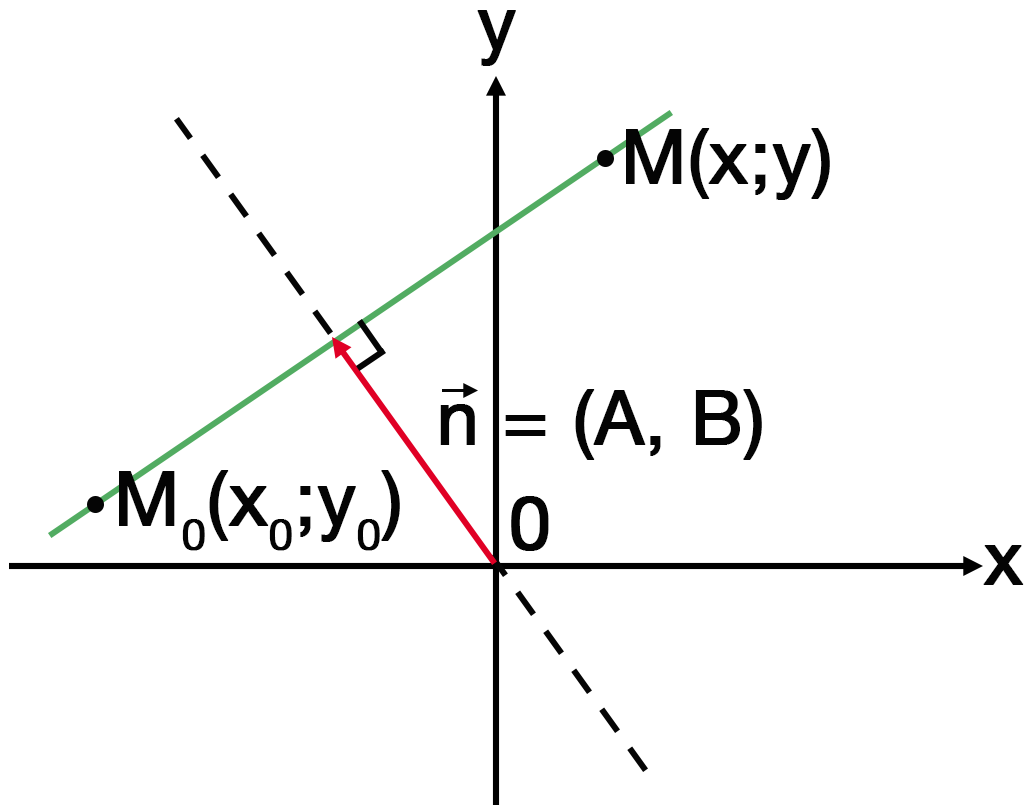
\includegraphics[width=0.5\textwidth]{general_line.png}
    \end{center}

    Следовательно, уравнение \(A(x - x_0) + B(y - y_0) = 0\) определяет некоторую прямую в прямоугольной системе координат на плоскости, а значит и эквивалентное ему уравнение \(Ax + By + C = 0\) определяет ту же прямую. \\

    \textbf{Пункт 2}. Любую прямую в прямоугольной системе координат на плоскости можно задать уравнением первой степени \(Ax + By + C = 0\). \\

    Зададим в прямоугольной системе координат на плоскости прямую \(a \); точку \(M_0(x_0, y_0)\), через которую проходит эта прямая, а также нормальный вектор этой прямой \(\vv{n} = (A, B)\).
    Пусть точка \(M(x, y)\) — произвольная точка на прямой, тогда векторы \(\vv{n} = (A, B)\) и \(\vv{M_0M} = (x - x_0, y - y_0)\) являются перпендикулярными друг другу и их скалярное произведение равно нулю:
    \begin{gather*}
        (\vv{n}, \vv{M_0M}) = A(x - x_0) + B(y - y_0) = 0
    \end{gather*}

    Пусть \(C = -Ax_0 - By_0\), тогда получим уравнение:
    \begin{gather*}
        Ax + By + C = 0
    \end{gather*}
\end{proof}

\subsection{Уравнение прямой в отрезках на осях}

Рассмотрим общее уравнение прямой \(Ax + By + C = 0\) при условии \(A \neq 0, B \neq 0, C \neq 0\) (то есть прямая не параллельна ни одной из осей координат и не проходит через начало отсчёта).
Теперь преобразуем уравнение:

\begin{gather*}
    Ax + By + C = 0  \iff Ax + By = -C \iff \frac{x}{\frac{-C}{A}} + \frac{y}{\frac{-C}{B}} = 1
\end{gather*}

\begin{center}
    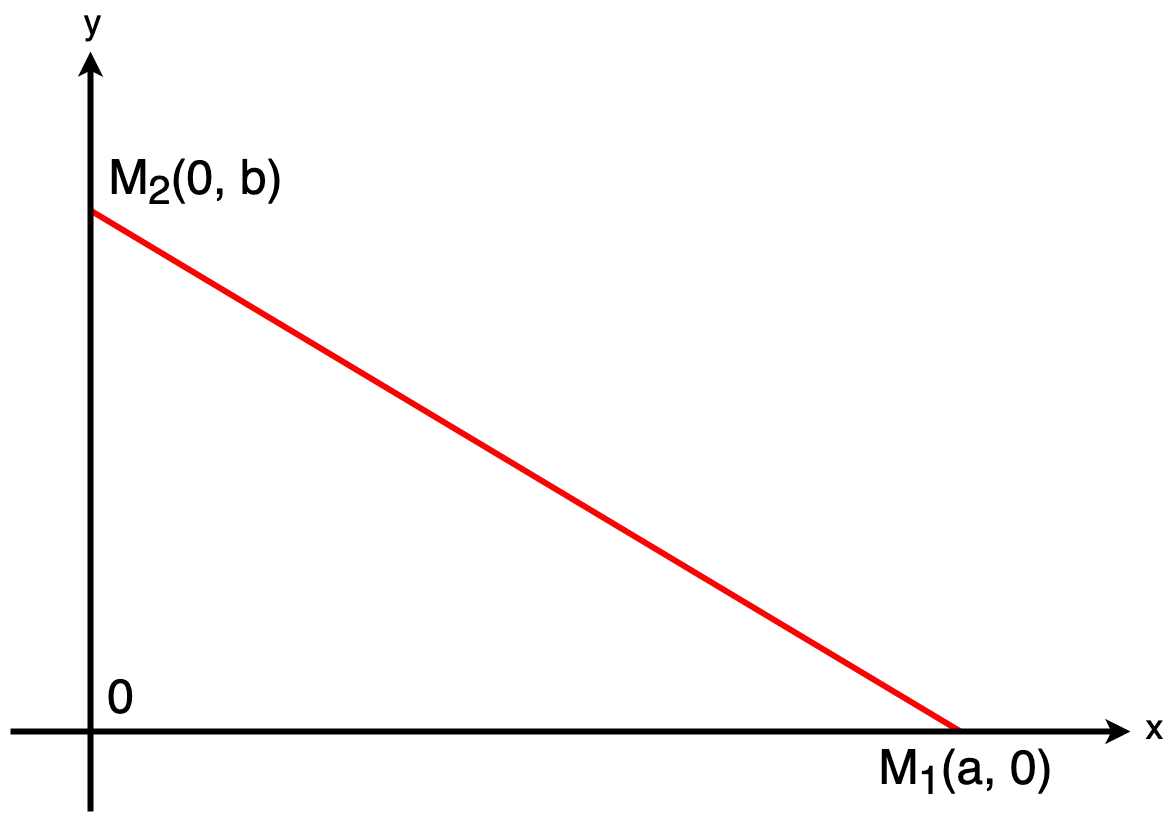
\includegraphics[width=0.7\textwidth]{axis_line.png}
\end{center}

Введем обозначение: \(\frac{-C}{A} = a\), \(\frac{-C}{B} = b\).
Отсюда получим уравнение:
\begin{gather*}
    \frac{x}{a} + \frac{y}{b} = 1
\end{gather*}

Это — уравнение прямой в отрезках на осях, так как числа \(a\) и \(b\) соответствуют длинам отрезков (с соответствующими знаками), которые прямая отсекает на осях координат (считая от начала отсчёта).

\section{Условия параллельности и перпендикулярности плоскостей и прямых в пространстве}
\label{sec:parallel_perpendicular_planes}

\subsection{Параллельность и перпендикулярность плоскостей}
Условия параллельности и перпендикулярности двух плоскостей равносильны условиям параллельности и перпендикулярности \textbf{их нормальных векторов}.

Пусть есть две плоскости:
\begin{gather*}
    \alpha: A_1x + B_1y + C_1z + D_1 = 0 \\
    \beta: A_2x + B_2y + C_2z + D_2 = 0
\end{gather*}

Тогда они:
\begin{itemize}
    \item[—]{\textbf{Перпендикулярны}, если \(A_1A_2 + B_1B_2 + C_1C_2 = 0\)}
    \item[—]{\textbf{Параллельны}, когда \(\dfrac{A_1}{A_2} = \dfrac{B_1}{B_2} = \dfrac{C_1}{C_2}\)}
\end{itemize}

\subsection{Параллельность и перпендикулярность прямых в пространстве}
В пространстве для прямых действуют те же условия, что и на плоскости, добавляется лишь новая координата.

\plink{sec:parallel_perpendicular_lines}{Перейти к параллельности и перпендикулярности прямых в пространстве}

\subsection{Параллельность и перпендикулярность прямой и плоскости}
Пусть есть прямая:
\begin{gather*}
    l: \frac{x - x_0}{m} = \frac{y - y_0}{n} = \frac{z - z_0}{p}
\end{gather*}

Ее направляющим вектором является вектор \(\vv{s} = (m, n, p)\).

И плоскость:
\begin{gather*}
    \alpha: Ax + By + Cz + D = 0
\end{gather*}

Ее нормальным вектором является вектор \(\vv{n} = (A, B, C)\)

Тогда прямая \textbf{параллельна} плоскости, когда:
\begin{gather*}
    \vv{n} \perp \vv{s} \iff \vv{n} \cdot \vv{s} = 0 \iff Am + Bm + Cp = 0
\end{gather*}

И прямая \textbf{перпендикулярна} плоскости, если:
\begin{gather*}
    \frac{A}{m} = \frac{B}{n} = \frac{C}{p}
\end{gather*}

\section{Условия параллельности и перпендикулярности прямых на плоскости}
\label{sec:parallel_perpendicular_lines}

Условия параллельности и перпендикулярности двух прямых равносильны условиям параллельности и перпендикулярности \textbf{их направляющих векторов}.

\subsection{Прямые, заданые в общем виде}
Пусть даны прямые, заданные общими уравнениями:
\begin{gather*}
    l_1: A_1x + B_1y + C_1 = 0 \\
    l_2: A_2x + B_2y + C_2 = 0
\end{gather*}

Тогда они:
\begin{itemize}
    \item[—]{\textbf{Перпендикулярны}, если \(A_1A_2 + B_1B_2 = 0\) (условие коллинеарности векторов).}
    \item[—]{\textbf{Параллельны}, когда \(\dfrac{A_1}{A_2} = \dfrac{B_1}{B_2} \neq \dfrac{C_1}{C_2}\) (условие параллельности векторов).}
    \item[—]{\textbf{Совпадают}, если \(\dfrac{A_1}{A_2} = \dfrac{B_1}{B_2} = \dfrac{C_1}{C_2}\).}
\end{itemize}

\subsection{Прямые с угловым коэффициентом}
Пусть даны прямые:
\begin{gather*}
    l_1: y = k_1x + b_1 \\
    l_2: y = k_2x + b_2
\end{gather*}

Тогда они:
\begin{itemize}
    \item[—]{\textbf{Перпендикулярны}, если \(k_1 = -\dfrac{1}{k_2}\)}
    \item[—]{\textbf{Параллельны}, когда \(k_1 = k_2\) при \(b_1 \neq b_2\)}
\end{itemize}

\subsection{Прямые, заданные каноническими уравнениями}
Пусть даны прямые, через каноническими уравнениями:
\begin{gather*}
    l_1: \frac{x - x_1}{m_1} = \frac{y - y_1}{n_1} \\
    l_2: \frac{x - x_2}{m_2} = \frac{y - y_2}{n_2}
\end{gather*}

Тогда они:
\begin{itemize}
    \item[—]{\textbf{Перпендикулярны}, когда \(m_1m_2 + n_1n_2 = 0\)}
    \item[—]{\textbf{Параллельны}, если \(\dfrac{m_1}{m_2} = \dfrac{n_1}{n_2}\)}
\end{itemize}

\chapter{Кривые второго порядка}%
\label{cha:Кривые второго порядка}

\section{Эллипс. Определение, вывод уравнения, характеристики}%
\label{sec:Эллипс. Определение, вывод уравнения, характеристики}

\begin{definition}
    Эллипсом называется геометрическое место точек плоскости, сумма расстояний от каждой из которых до двух заданных точек есть величина постоянная

    Обозначим соответствующие точки через \(F_1\) и \(F_2\), тогда условие, сформулированное в определении для произвольной точки эллипса \(M\) можно записать следующим образом:
    \[
        |F_1 M| + |F_2 M| = const
    \]

    Вводя краткие обозначения
    \[
        |F_1 M| = r_1, \quad |F_2 M| = r_2, \quad |F_1 F_2| = 2c, \quad const = 2a, \quad a > 0
    \]
    получаем
    \[
        r_1 + r_2 = 2a, \quad c < a
    \]
    \begin{note}
        Из определения следует, что эллипс — ограниченная кривая:
        \[
            \frac{x^2}{a^2} = 1 - \frac{y^2}{b^2} \quad \implies \quad \Big| \frac{x}{a} \Big| \leq 1 \quad \implies \quad |x| \leq a, \quad x = \pm a \quad y = 0
        \]
        \[
            \frac{y^2}{b^2} = 1 - \frac{x^2}{a^2} \quad \implies \quad \Big| \frac{y}{b} \Big| \leq 1 \quad \implies \quad |y| \leq b, \quad y = \pm b \quad x = 0
        \]
    \end{note}

    \begin{note}
        Симметрия эллипса: осевая и центральная
        \[
            M(x, y) \in E \quad \implies \quad M_1 (x, -y) \in E, \quad M_2 (-x, y) \in E, \quad M_3 (-x, -y) \in E
        \]
    \end{note}

    \begin{note}
        Точки пересечения эллипса с осями координат:
        \[
            A_1 (-a, 0), \quad A_2 (a, 0), \quad B_1 (0, -b), \quad B_2 (0, b)
        \]
    \end{note}
\end{definition}

\subsection{Определения}%
\label{sub:Определения}
\begin{itemize}
    \item {Точки \(F_1\) и \(F_2\) называются \textbf{фокусами} эллипса.}
    \item {Расстояние \(c = \dfrac{|F_1 F_2|}{2}\) называется \textbf{фокусным расстоянием}.}
    \item {Точки \(A_1, A_2, B_1, B_2\) называются \textbf{вершинами} эллипса.}
    \item {Отрезок \(A_1 A_2\) \((B_1 B_2)\) называется \textbf{большой (малой) осью эллипса.}}
    \item {Величина \(2a\) \((2b)\) называется \textbf{длиной большой (малой)} оси.}
    \item {Величина \(\varepsilon = \dfrac{c}{a}\) называется \textbf{эксцентриситетом} эллипса.}
    \item {\textbf{Директрисами эллипса} называются прямые, параллельные малой оси эллипса и проходящие от на на расстоянии \(\dfrac{a}{\varepsilon}\)}
\end{itemize}

\begin{note}
    Эксцентриситет \(\varepsilon\):
    \[
        a > c \quad \implies \quad \varepsilon = \frac{c}{a} \quad \implies \quad \varepsilon \in [0, 1)
    \]
    Частные случаи:
    \[
        \varepsilon = 0 \; \implies \; c = 0 \; \implies \; F_1 = F_2 \; \implies \; r_1 = r_2 = a = R \text{ — окружность}
    \]
    \[
        \varepsilon = 0 \; \implies \; b = 0 \; \implies \; |F_1 F_2| = 2a \; \implies \; F_1 F_2 \text{ — отрезок}
    \]
\end{note}

\subsection{Каноническое уравнение эллипса}%
\label{sub:Каноническое уравнение эллипса}

\begin{siderules}
    Канонической системой координат для эллипса называется декартова прямоугольная система координат, центр которой является серединой отрезка, заключенного между точками \(F_1\) и \(F_2\), которые лежат на оси \(Ox\).
\end{siderules}

\begin{lemma}
    Уравнение эллипса в канонической системе координат имеет вид:
    \[
        \frac{x^2}{a^2} + \frac{y^2}{b^2} = 1
    \]

    и называется \textbf{каноническим уравнением} эллипса.
\end{lemma}

\begin{proof}
    Подставим в определение эллипса выражения для \(r_1\) и \(r_2\):
    \[
        r_1 = \sqrt{{(x + c)}^2 + y^2}, \quad r_2 = \sqrt{{(c - x)}^2 + y^2}
    \]
    Тогда:
    \begin{gather*}
        \sqrt{{(x + c)}^2 + y^2} + \sqrt{{(c - x)}^2 + y^2} = 2a \\
        {(x + c)}^2 + y^2 = 4a^2 - 4a \sqrt{{(c - x)}^2 + y^2} + {(c - x)}^2 + y^2 \\
        4xc = 4a^2 - 4a \sqrt{{(c - x)}^2 + y^2} \\
        a^2 - xc = a \sqrt{{(c - x)}^2 + y^2} \\
        x^2 (a^2 - c^2) + a^2 y^2 = a^2 (a^2 - c^2) \\
        \frac{x^2}{a^2} + \frac{y^2}{(a^2 - c^2)} = 1
    \end{gather*}

    Заметим, что \(b^2 = a^2 - c^2 > 0\), откуда получаем искомое уравнение.
\end{proof}

\begin{lemma}
    Всякое уравнение вида \(\dfrac{x^2}{a^2} + \dfrac{y^2}{b^2} = 1\) определяет эллипс.
\end{lemma}

\begin{proof}
    Покажем, что из канонического уравнения эллипса следуют геометрические соотношения, лежащие в основе его определения.

    Имеем:
    \[
        y^2 = b^2 \Big(1 - \frac{x^2}{a^2}\Big)
    \]
    \[
        r_{1, 2} = \sqrt{(x \pm c)^2 + b^2 - \frac{b^2}{a^2} x^2} =
        \sqrt{\Big(1 - \frac{b^2}{a^2}\Big) x^2 \pm 2xc + a^2} =
        \sqrt{\Big(\frac{c}{a}x \pm a\Big)^2} = \Big| \frac{c}{a}x \pm a \Big|
    \]
    Откуда получаем:
    \[
        r_1 = a + \varepsilon x, \quad r_2 = a - \varepsilon x, \quad \varepsilon = \frac{c}{a}
    \]
    Тогда:
    \[
        r_1 + r_2 = 2a
    \]
\end{proof}

\subsection{Рациональное уравнение эллипса}%
\label{sub:Рациональное уравнение эллипса}

\begin{siderules}
    Рациональными уравнениями эллипса называются уравнения вида:
    \[
        r_1  = a + \varepsilon x, \quad r_2 = a - \varepsilon x, \quad \varepsilon = \frac{c}{a}
    \]
\end{siderules}

\subsection{Полярное уравнение эллипса}%
\label{sub:Полярное уравнение эллипса}

\begin{siderules}
    Полярным уравнением эллипса называется уравнение вида:
    \[
        \rho  = \frac{p}{1 - \varepsilon \cos{\varphi}}, \quad p = a - \varepsilon c
    \]
    где \((\rho, \varphi)\) — полярные координаты на плоскости, \(F_1\) — полюс и \(Ox\) — полярная ось.
\end{siderules}

\begin{lemma}
    Полярное уравнение эллипса \(\rho = \dfrac{p}{1 - \varepsilon \cos{\varphi}}\) задает эллипс.
\end{lemma}

\begin{proof}
    Из определения эллипса следует, что \(|F_1 M| + |F_2 M| = 2a\), \(|F_1 F_2| = 2c\). Кроме того, поскольку \(F_1\) является полюсом, то \(F_1M = \rho\).

    Пусть угол между \(\varphi = \angle{(F_1M, F_1F_2)}\). Тогда по теореме косинусов:
    \begin{gather*}
        F_2 M = \sqrt{F_1M^2 + F_1F_2^2 - 2F_1F_2\cos{\varphi}} \\
        F_2 M = \sqrt{\rho^2 + 4c^2 - 4c\rho\cos{\varphi}}
    \end{gather*}

    \begin{center}
        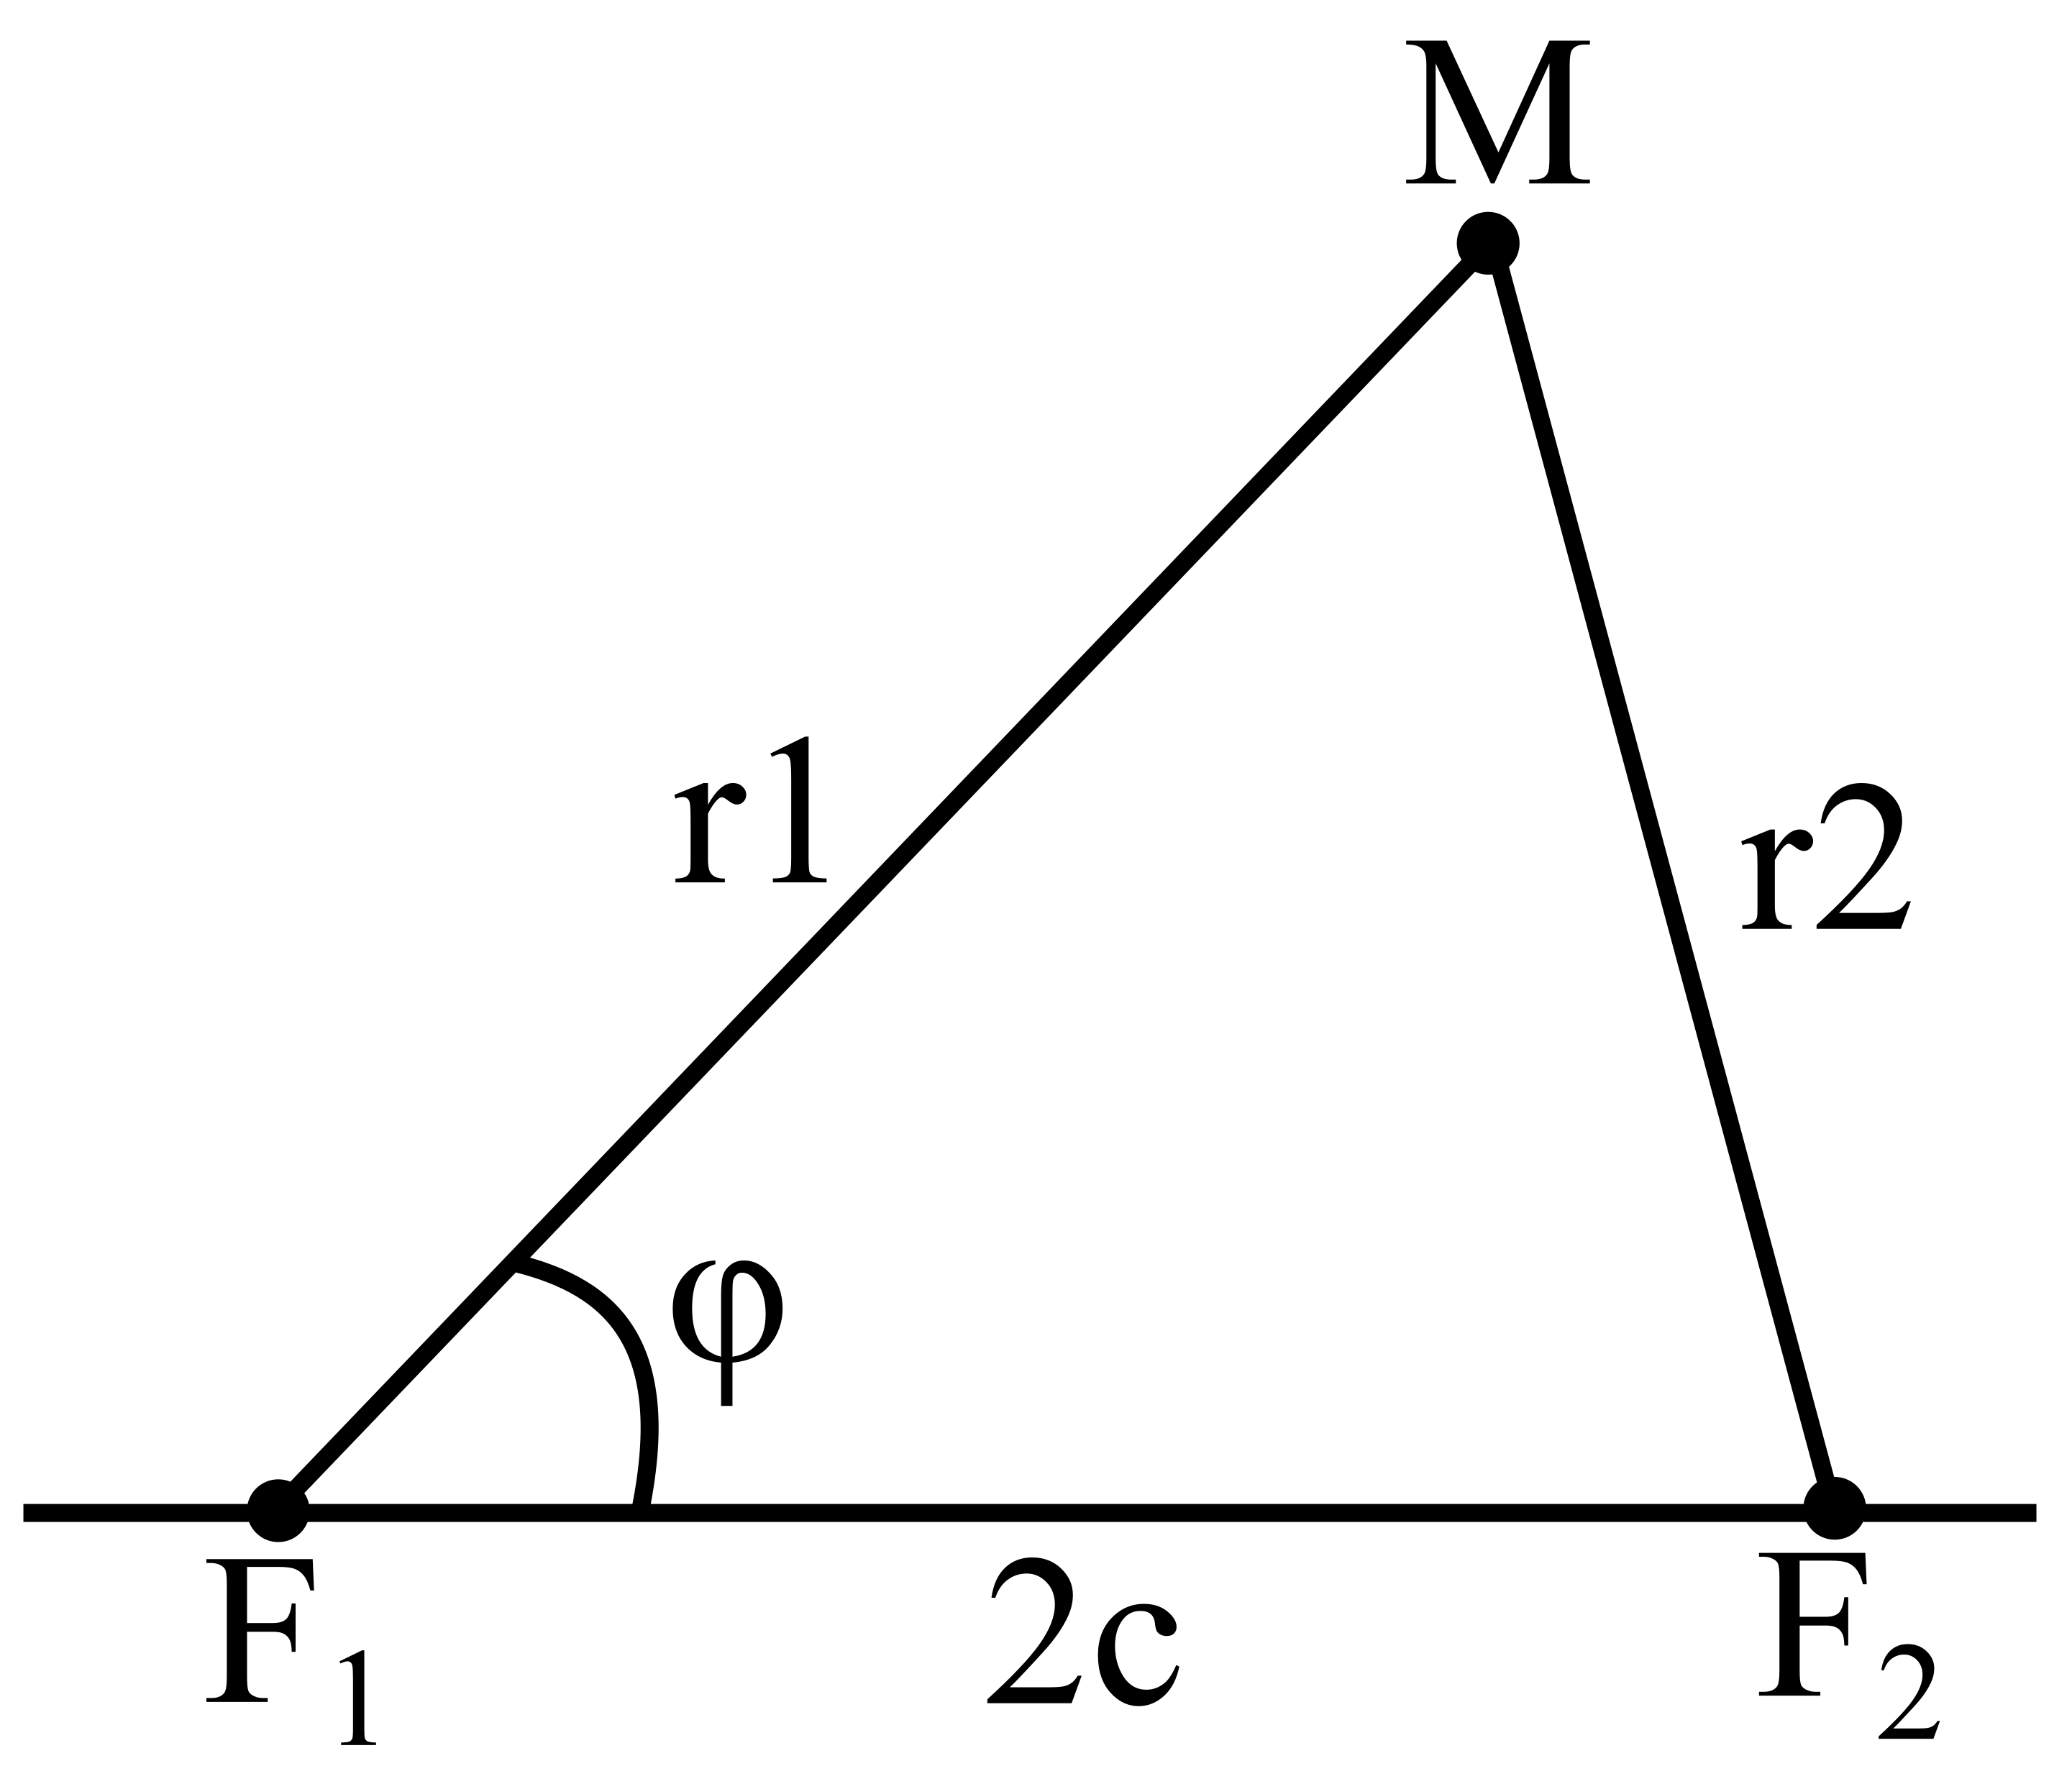
\includegraphics[width=0.4\textwidth]{polar_cos.png}
    \end{center}

    Тогда:
    \begin{gather*}
        F_1M + F_2M = 2a \\
        \rho + \sqrt{\rho^2 + 4c^2 - 4c\rho\cos{\varphi}} = 2a \\
        \rho^2 + 4c^2 - 4c\rho\cos{\varphi} = \rho^2 - 4a\rho + 4a^2 \\
        c^2 - c\rho\cos{\varphi} = -a\rho + a^2 \\
        a\rho (1 - \frac{c}{a}\cos{\varphi}) = a^2 - c^2
    \end{gather*}

    Вспомним обозначения: \(\varepsilon = \dfrac{a}{c}, p = a - \varepsilon c\). Значит:
    \begin{gather*}
        \rho(1 - \varepsilon\cos{\varphi}) = p \\
        \rho = \frac{p}{1 - \varepsilon\cos{\varphi}}
    \end{gather*}
\end{proof}

\subsection{Параметрическое уравнение эллипса}%
\label{sub:Параметрическое уравнение эллипса}

\begin{siderules}
    Параметрическим уравнением эллипса называются уравнения вида
    \[
        x(t) = a \cdot \cos{t}, \quad y(t) = b \cdot \sin{t}
    \]
\end{siderules}

\begin{lemma}
    Параметрические уравнения эллипса задают эллипс.
\end{lemma}

\begin{proof}
    Имеет место следующее тождество:
    \[
        \frac{{x(t)}^2}{a^2} + \frac{{y(t)}^2}{b^2} = \cos^2{t} + \sin^2{t} = 1
    \]
\end{proof}

\section{Гипербола. Определение, вывод уравнения, характеристики}%
\label{sec:Гипербола. Определение, вывод уравнения, характеристики}

\begin{definition}
    Гиперболой называется геометрическое место точек плоскости, модуль разности расстояний от каждой из которых до двух заданных точек плоскости есть величина постоянная.

    Обозначим соответствующие точки через \(F_1\) и \(F_2\).
    Пусть \(M\) — произвольная точка гиперболы, тогда условие, сформулированное в определении, можно записать следующим образом:
    \[
        ||F_1 M| - |F_2 M|| = const
    \]

    Вводя краткие обозначения
    \[
        |F_1 M| = r_1, \quad |F_2 M| = r_2, \quad |F_1 F_2| = 2c, \quad const = 2a, \quad a > 0
    \]

    получаем
    \[
        |r_1 - r_2| = 2a, \quad c > a
    \]

    что приводит к двум уравнениям:
    \begin{gather*}
        r_1 - r_2 = 2a, \quad r_1 > r_2 \\
        r_2 - r_1 = 2a, \quad r_2 > r_1
    \end{gather*}

    Гипербола — неограниченная кривая:
    \[
        \frac{x^2}{a^2} = 1 + \frac{y^2}{b^2} \quad \implies \quad \Big|\frac{x}{a}\Big| \geq 1 \quad \implies \quad |x| \geq a, \quad x = \pm a \quad y = 0
    \]
    \[
        \frac{y^2}{b^2} = \frac{x^2}{a^2} - 1 \quad \implies \quad \Big|\frac{y}{b}\Big| \geq 1 \quad \implies \quad |y| \geq 0, \quad y = \pm b \quad x = 0
    \]

    Осевая и центральная симметрии
    \[
        M(x, y) \in H \quad \implies \quad M_1 (x, -y) \in H, \quad M_2 (-x, y) \in H, \quad M_3 (-x, -y) \in H
    \]

    Точки пересечения с осями координат и вспомогательные точки:
    \[
        A_1 (-a, 0), \quad A_2 (a, 0), \quad B_1 (0, -b), \quad B_2 (0, b)
    \]
\end{definition}

\subsection{Определения}%
\label{sub:Определения}

\begin{itemize}
    \item {Точки \(F_1\) и \(F_2\) называются \textbf{фокусами} гиперболы.}
    \item {Расстояние \(c = \dfrac{|F_1 F_2|}{2}\) называется \textbf{фокусным расстоянием}.}
    \item {Точки \(A_1\), \(A_2\) называются \textbf{вершинами} гиперболы.}
    \item {Отрезок \(A_1 A_2\) \((B_1 B_2)\) называется \textbf{вещественной (мнимой)} осью гиперболы.}
    \item {Величина \(2a\) \((2b)\) называется \textbf{длиной вещественной (мнимой)} оси.}
    \item {Величина \(e = \dfrac{c}{a}\) называется \textbf{эксцентриситетом} гиперболы.}
    \item {
          \textbf{Директрисами гиперболы} называются прямые, параллельные ее мнимой оси и находящиеся на расстоянии \(\dfrac{a}{\varepsilon}\):
          \[
              x = \pm \dfrac{a}{\varepsilon}, \quad \varepsilon > 1
          \]
          }
\end{itemize}

\subsection{Каноническое уравнение гиперболы}%
\label{sub:Каноническое уравнение гиперболы}
\begin{siderules}
    Каноническая система координат для гиперболы — это прямоугольная декартова система координат, центр которой является серединой отрезка, заключенного между точками \(F_1\) и \(F_2\), которые лежат на оси \(Ox\).
\end{siderules}

\begin{lemma}
    Уравнение гиперболы в канонической системе координат имеет вид:
    \[
        \frac{x^2}{a^2} - \frac{y^2}{b^2} = 1
    \]
    и называется \textbf{каноническим уравнением} гиперболы.
\end{lemma}

\begin{proof}
    Подставим в определение гиперболы выражения для \(r_1\) и \(r_2\):
    \[
        r_1 = \sqrt{{(x + c)}^2 + y^2}, \quad r_2 = \sqrt{{(c - x)}^2 + y^2}
    \]
    Будем иметь:
    \begin{gather*}
        \sqrt{{(x + c)}^2 + y^2} - \sqrt{{(c - x)}^2 + y^2} = 2a \\
        {(x + c)}^2 + y^2 = 4a^2 + 4a \sqrt{{(c - x)}^2 + y^2} + {(c - x)}^2 + y^2 \\
        4xc = 4a^2 + 4a \sqrt{{(c - x)}^2 + y^2} \\
        xc - a^2 = a \sqrt{{(c - x)}^2 + y^2}
        x^2 (c^2 - a^2) - a^2 y^2 = a^2 (c^2 - a^2) \\
        \frac{x^2}{a^2} - \frac{y^2}{(c^2 - a^2)} = 1
    \end{gather*}
    Заметим, что \(b^2 = c^2 - a^2 > 0\), откуда получаем искомое уравнение.
\end{proof}

\begin{lemma}
    Всякое уравнение вида \(\dfrac{x^2}{a^2} - \dfrac{y^2}{b^2} = 1\) определяет гиперболу.
\end{lemma}

\begin{proof}
    Покажем, что из канонического уравнения гиперболы следуют геометрические соотношения, лежащие в основе определения. Имеем:
    \[
        y^2 = b^2 \Big(\frac{x^2}{a^2} - 1\Big)
    \]
    \[
        r_{1, 2} = \sqrt{{(x \pm c)}^2 + \frac{b^2}{a^2} x^2 - b^2} = \sqrt{\Big(1 + \frac{b^2}{a^2}\Big) x^2 \pm 2xc + a^2} = \sqrt{\Big(\frac{c}{a}x \pm a\Big)^2} = \Big| \frac{c}{a}x \pm a \Big|
    \]
    Откуда получаем:
    \[
        r_1 = \varepsilon x + a, \quad r_2 = \varepsilon x - a, \quad r_1 > r_2
    \]
    \[
        r_1 = -\varepsilon x + a, \quad r_2 = -\varepsilon x - a, \quad r_1 < r_2
    \]
\end{proof}

\subsection{Рациональное уравнение гиперболы}%
\label{sub:Рациональное уравнение гиперболы}

\begin{siderules}
    Рациональными уравнениями гиперболы называются уравнения вида:
    \begin{gather*}
        r_1 = \varepsilon x + a, \quad r_2 = \varepsilon x - a \\
        r_1 = -\varepsilon x + a, \quad r_2 = -\varepsilon x - a
    \end{gather*}
    где величина \(\varepsilon = \dfrac{c}{a}\) называется \textbf{эксцентриситетом гиперболы}.
\end{siderules}

\begin{note}
    Эксцентриситет \(\varepsilon\):
    \[
        a < c \quad \implies \quad \varepsilon = \frac{c}{a} \quad \implies \quad \varepsilon \in [1, +\infty).
    \]
    Частные случаи:
    \[
        \varepsilon = 1 \quad \implies \quad b = 0 \text{ — лучи из фокусов}
    \]
    \[
        \varepsilon = +\infty \quad \implies \quad a = 0 \text{ — ось } Oy
    \]
\end{note}

\subsection{Полярное уравнение гиперболы}%
\label{sub:Полярное уравнение гиперболы}

\begin{siderules}
    Полярными уравнениями гиперболы называются уравнения вида
    \begin{gather*}
        \rho = \frac{p}{1 - \varepsilon \cos{\varphi}}, \quad p = a - \varepsilon c, \quad r_1 > r_2 \\
        \rho = -\frac{p}{1 - \varepsilon \cos{\varphi}}, \quad p = a - \varepsilon c, \quad r_1 < r_2
    \end{gather*}
    где \((\rho, \varphi)\) — полярные координаты на плоскости, \(F_1\) — полюс и \(Ox\) — полярная ось.
\end{siderules}

\begin{lemma}
    Полярное уравнение гиперболы задает гиперболу
\end{lemma}

\begin{proof}
    Рассмотрим случай при \(r_1 > r_2\). Случай при \(r_2 > r_1\) доказывается аналогично.

    Из определения гиперболы следует, что \(|F_1 M| - |F_2 M| = 2a\), \(|F_1 F_2| = 2c\). Кроме того, поскольку \(F_1\) является полюсом, то \(F_1M = \rho\).

    Пусть угол между \(\varphi = \angle{(F_1M, F_1F_2)}\). Тогда по теореме косинусов:
    \begin{gather*}
        F_2 M = \sqrt{F_1M^2 + F_1F_2^2 - 2F_1F_2\cos{\varphi}} \\
        F_2 M = \sqrt{\rho^2 + 4c^2 - 4c\rho\cos{\varphi}}
    \end{gather*}

    \begin{center}
        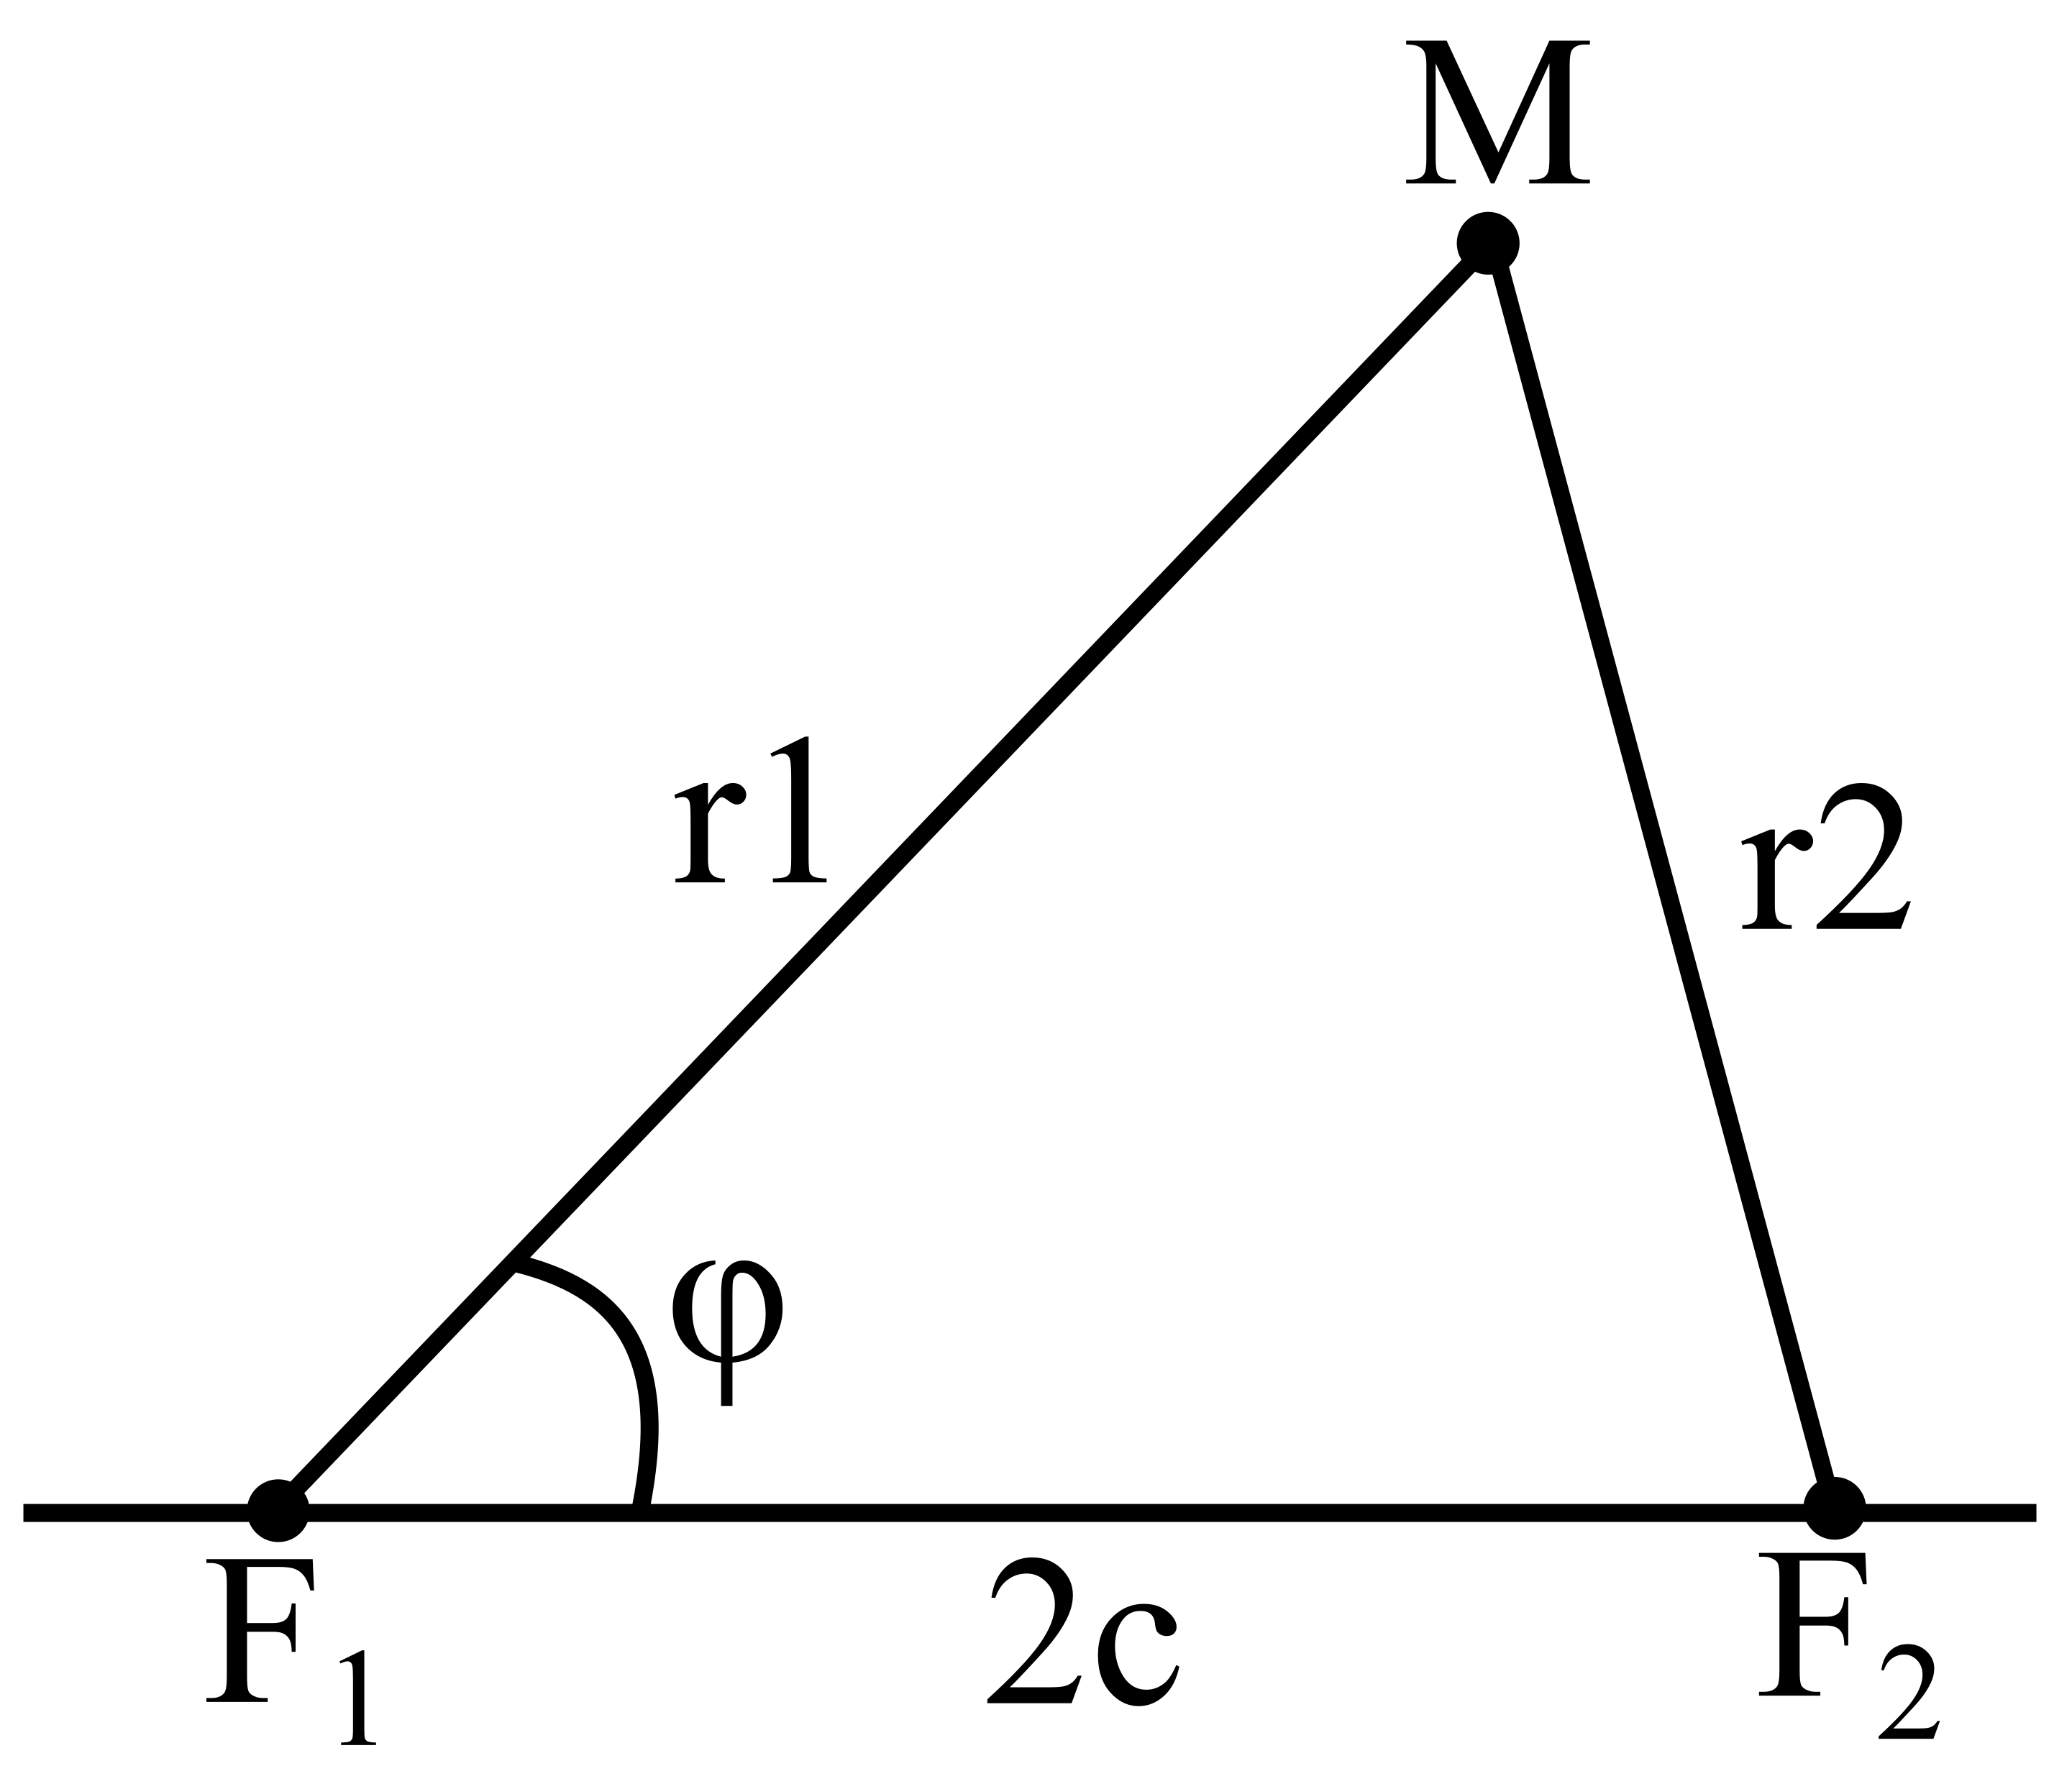
\includegraphics[width=0.4\textwidth]{polar_cos.png}
    \end{center}

    Тогда:
    \begin{gather*}
        F_1M - F_2M = 2a \\
        \rho - \sqrt{\rho^2 + 4c^2 - 4c\rho\cos{\varphi}} = 2a \\
        \rho^2 + 4c^2 - 4c\rho\cos{\varphi} = \rho^2 - 4a\rho + 4a^2 \\
        c^2 - c\rho\cos{\varphi} = -a\rho + a^2 \\
        a\rho (1 - \frac{c}{a}\cos{\varphi}) = a^2 - c^2
    \end{gather*}

    Вспомним обозначения: \(\varepsilon = \dfrac{a}{c}, p = a - \varepsilon c\). Значит:
    \begin{gather*}
        \rho(1 - \varepsilon\cos{\varphi}) = p \\
        \rho = \frac{p}{1 - \varepsilon\cos{\varphi}}
    \end{gather*}
\end{proof}

\subsection{Параметрическое уравнение гиперболы}%
\label{sub:Параметрическое уравнение гиперболы}

\begin{siderules}
    Параметрическими уравнениями гиперболы называются уравнения вида
    \[
        x(t) = a \cdot \cosh{t}, \quad y(t) = b \cdot \sinh{t}
    \]
\end{siderules}

\begin{lemma}
    Параметрические уравнения гиперболы задают гиперболу.
\end{lemma}

\begin{proof}
    Имеет место следующее тождество:
    \[
        \frac{x(t)^2}{a^2} - \frac{y(t)^2}{b^2} = \cosh^2{t} - \sinh^2{t} = 1
    \]
\end{proof}

\section{Парабола. Определение, вывод уравнения, характеристики}
\label{sec:parabola}

\subsection{Определение}
Парабола — геометрическое место точек на плоскости, равноудалённых от данной прямой \(d\) и данной точки \(F\).
Точка \(F\) не лежит ни на кривой, ни на прямой \(d\).

Точка \(F\) называется \textbf{фокусом}, а прямая \(d\) — \textbf{директрисой параболы}.
Расстояние от фокуса до директрисы называется \textbf{фокальным параметром} параболы и обозначается через \(p\).

\textbf{Эксцентриситет} параболы — это отношение расстояний от произвольной точки на кривой до фокуса и от этой же точки до директрисы.
Эксцентриситет параболы по определению равен 1.

Каноническое уравнение параболы: \(y^2 = 2px\)

\subsection{Вывод канонического уравнения}

Пусть фокус \(F\) принадлежит оси \(OX\).
Проведем директрису перпендикулярно оси \(OX\) на расстоянии \(p\) от фокуса \(F\), тогда пусть т. \(O\) будет серединой этого расстояния.
Возьмем т. \(M(x; y)\), которая принадлежит параболе.
Расстояние от т. \(M(x; y)\) до фокуса обозначим за \(r\), до директрисы за \(d\).

\begin{center}
    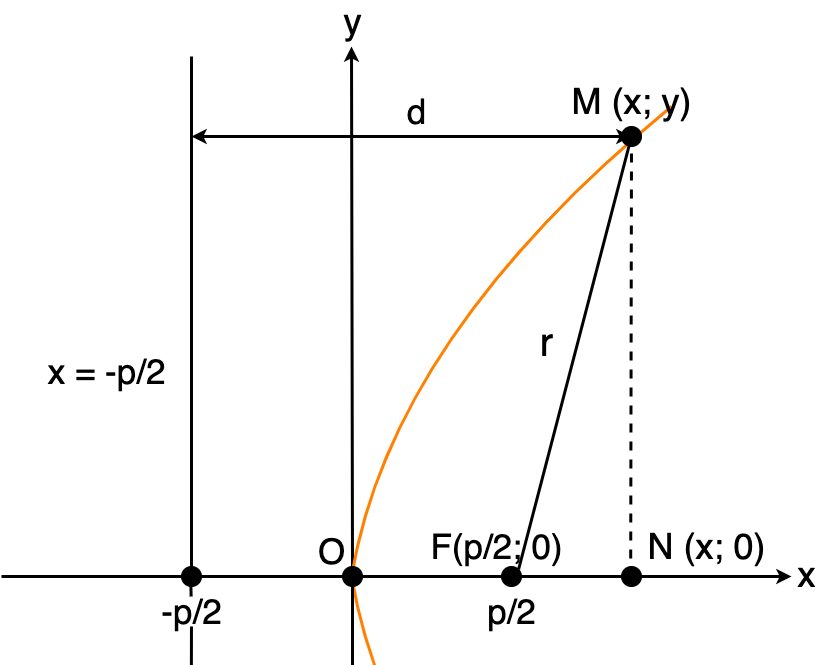
\includegraphics[width=0.8\textwidth]{parabola.png}
\end{center}

Расстояние от т. \(M(x;y)\) до директрисы равно \(d = \Big| x + \dfrac{p}{2} \Big| \).

По определению параболы \(r = d\).

По теореме Пифагора из прямоугольного \(\Delta FMN\): \(r=\sqrt{\Big(x - \dfrac{p}{2}\Big)^2 + y^2}\)

Следовательно:

\begin{gather*}
    \sqrt{\Big(x - \frac{p}{2}\Big)^2 + y^2} = x + \frac{p}{2} \\
    x^2 - px + \frac{p^2}{4} + y^2 = x^2 + px + \frac{p^2}{4} \\
    y^2 = 2px
\end{gather*}

\subsection{Уравнение в полярной системе координат}

Выберем фокус \(F\) параболы, а в качестве полярной оси — луч с началом в точке \(F\), перпендикулярный директрисе и не пересекающий её.
Тогда для произвольной точки \(M(r, \varphi)\), принадлежащей параболе, по определению \(d = r\).

\begin{center}
    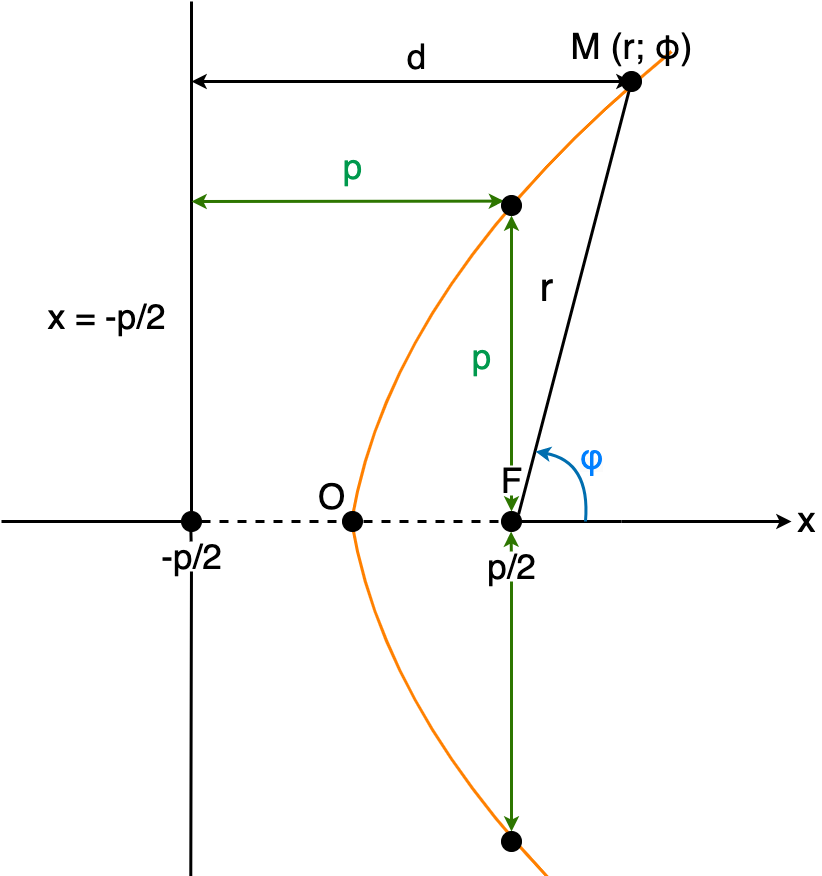
\includegraphics[width=0.7\textwidth]{parabola2.png}
\end{center}

Поскольку \(d = p + r\cos{\varphi}\), получим уравнение параболы в координатной форме:
\begin{gather*}
    d = p + r \cdot \cos{\varphi}  \iff r = \dfrac{p}{1 - \cos{\varphi}}
\end{gather*}

что является уравнением параболы в полярной системе координат \(Fr\varphi\).

\subsection{Свойства параболы}

\begin{itemize}
    \item[—]{Имеет ось симметрии называемой осью параболы. Ось проходит через фокус и вершину перпендикулярно директрисе;}
    \item[—]{Если фокус параболы отразить относительно касательной, то его образ будет лежать на директрисе;}
    \item[—]{Все параболы подобны. Расстояние между фокусом и директрисой определяет масштаб;}
\end{itemize}

\chapter{Множества и последовательности}%
\label{cha:Множества и последовательности}

\section{Последовательность}%
\label{sec:Последовательность}

\subsection{Определение}%
\label{sub:Определение}

\begin{siderules}
    Числовая последовательность \(\{x_n\}\) — это правило, согласно которому каждому натуральному числу \(n = 1, 2, 3, ...\) ставится в соответствие число \(x_n\). Число \(x_n\) называют \(n\)-ным членом или элементом последовательности.
\end{siderules}

Другими словами числовая последовательность – это функция, областью определения которой является множество натуральных чисел. Число элементов последовательности бесконечно. Среди элементов могут встречаться и члены, имеющие одинаковые значения. Также последовательность можно рассматривать как нумерованное множество чисел, состоящее из бесконечного числа членов.

\subsection{Ограниченная последовательность}%
\label{sub:Ограниченная последовательность}

\begin{siderules}
    Последовательность \(\{x_n\}\) называется \textbf{ограниченной}, если
    \[
        \exists M: \forall n \in \mathbb{N} \; |x_n| < M
    \]
\end{siderules}

\begin{siderules}
    \textbf{Верхней гранью \(\sup x_n\) последовательности \(\{x_n\}\)} называют наименьшее из чисел, ограничивающее последовательность сверху. То есть:
    \[
        \begin{cases}
            \exists M: \forall n \in \mathbb{N} \; x_n \leq M \\
            \forall M_1 < M \; \exists x_k: x_k > M_1
        \end{cases}
    \]
\end{siderules}

\begin{siderules}
    \textbf{Нижней гранью \(\inf x_n\) последовательности \(\{x_n\}\)} называют наибольшее из чисел, ограничивающее последовательность снизу. То есть:
    \[
        \begin{cases}
            \exists m: \forall n \in \mathbb{N} \; x_n \geq m \\
            \forall m_1 > m \; \exists x_k: x_k < m_1
        \end{cases}
    \]
\end{siderules}

\section{Предел последовательности}%
\label{sec:Предел последовательности}

\subsection{Определения}%
\label{sub:Определения}

\begin{siderules}
    Значение \(A\) называется пределом последовательности \(\{x_n\}\), если для любого сколь угодно малого числа \(\varepsilon\) найдется номер, начиная с которого все элементы последовательности будут отличаться от предела меньше чем на \(\varepsilon\).
    \[
        \lim_{n \to \infty}{x_n} = A \iff
        \forall \varepsilon > 0 \; \exists N_{\varepsilon} \in \mathbb{N}: \forall n \in \mathbb{N}: n \geq N \implies |x_n - A| < \varepsilon
    \]
    \(\varepsilon\)-окрестностью точки \(A\) называется открытый интервал \((A - \varepsilon, A + \varepsilon)\).
\end{siderules}

\begin{siderules}
    \textbf{Сходящаяся последовательность} — это последовательность, у которой существует предел. Если последовательность \(\{x_n\}\) имеет предел \(\displaystyle \lim_{n \to \infty}{x_n} = A\), то говорят, что последовательность \(\{x_n\}\) сходится к \(A\).
\end{siderules}

\begin{siderules}
    \textbf{Расходящаяся последовательность} — это последовательность, не имеющая предела.
\end{siderules}

\subsection{Свойства конечных пределов последовательности}%
\label{sub:Свойства конечных пределов последовательности}

\begin{property}
    Точка \(A\) является пределом последовательности \(\{x_n\}\) тогда и только тогда, когда за пределами любой окрестности этой точки находится находится конечное число элементов последовательности или пустое множество.
\end{property}

\begin{proof}
    Пусть точка \(A\) является пределом последовательности \(\{x-n\}\). Из определения следует, что:
    \[
        \lim_{n \to \infty}{x_n} = A \iff
        \forall \varepsilon > 0 \; \exists N_{\varepsilon} \in \mathbb{N}: \forall n \in \mathbb{N}: n \geq N \implies |x_n - A| < \varepsilon
    \]

    Тогда за пределами окрестности может находиться не более \(N\) элементов последовательности — конечное число или пустое множество.

    Докажем обратное. Пусть за пределами любой окрестности точки \(A\) находится конечное число элементов последовательности или пустое множество, а \(N - 1\) есть наибольший номер элемента, находящегося за пределами окрестности. Тогда все элементы последовательности с номерами \(n \geq N\) принадлежат этой окрестности. Следовательно точка \(A\) является пределом последовательности.
\end{proof}

\begin{property}
    Если число \(A\) не является пределом последовательности \(\{x_n\}\), то существует такая окрестность точки \(A\), за пределами которой находится бесконечное число элементов последовательности.
\end{property}

\begin{proof}
    Докажем от противного. Пусть \(A\) не является пределом последовательности \(\{x_n\}\) и за пределами любой окрестности точки \(A\) находится конечное число элементов последовательности. Рассмотрим произвольную окрестность точки \(A\): пусть \(N - 1\) есть наибольший номер элемента, находящегося за ее пределами. Тогда все элементы с номерами \(n \geq N\) принадлежат окрестности. Следовательно \(A\) является пределом последовательности. Получили противоречие, доказывающее свойство.
\end{proof}

\begin{theorem*}[единственности предела числовой последовательности]
    \newpar
    Если последовательность имеет предел, то он единственный
\end{theorem*}

\begin{proof}
    Докажем от противного. Пусть у последовательности \(\{x_n\}\) существует два разных предела:
    \[
        \begin{cases}
            \displaystyle
            \lim_{n \to \infty}{x_n} = A \\
            \displaystyle
            \lim_{n \to \infty}{x_n} = B \\
            A \neq B
        \end{cases}
    \]

    Тогда по определению предела:
    \[
        \lim_{n \to \infty}{x_n} = A \iff
        \forall \varepsilon > 0 \; \exists N_{A}(\varepsilon) \in \mathbb{N}: \forall n \in \mathbb{N}: n \geq N_{A}(\varepsilon) \implies |x_n - A| < \varepsilon
    \]
    \[
        \lim_{n \to \infty}{x_n} = B \iff
        \forall \varepsilon > 0 \; \exists N_{B}(\varepsilon) \in \mathbb{N}: \forall n \in \mathbb{N}: n \geq N_{B}(\varepsilon) \implies |x_n - B| < \varepsilon
    \]

    Следовательно элементы последовательности будут находиться в интервалах:
    \[
        \begin{cases}
            A - \varepsilon < x_n < A + \varepsilon \\
            B - \varepsilon < x_n < B + \varepsilon
        \end{cases}
    \]

    Пусть \(N = \max(N_{A}(\varepsilon), N_{B}(\varepsilon))\) и \(\varepsilon = \dfrac{|A - B|}{2}\). Тогда нетрудно убедиться, что эти два интервала не имеют общих точек. Однако, по определению предела все элементы последовательности при \(n > N\) должны находиться как в первом, так и во втором промежутке. Возникает противоречие, доказывающее теорему.
\end{proof}

\begin{theorem*}[об ограниченности последовательности, имеющей конечный предел]
    Если последовательность имеет конечный предел, то она ограничена.
\end{theorem*}

\begin{proof}
    Пусть последовательность \(\{x_n\}\) имеет конечный предел \(A\), тогда:
    \[
        \lim_{n \to \infty}{x_n} = A \iff
        \forall \varepsilon > 0 \; \exists N_{\varepsilon} \in \mathbb{N}: \forall n \in \mathbb{N}: n \geq N_{\varepsilon} \implies |x_n - A| < \varepsilon
    \]

    Из этого следует, что
    \[
        \forall n \geq N_{\varepsilon} \; A - \varepsilon < x_n < A + \varepsilon
    \]

    Кроме того, элементов с номером \(n < N_{\varepsilon}\) конечное число, поскольку \(N_{\varepsilon}\) — конечное число. Следовательно их значения ограничены некоторыми \(m_N\) и \(M_N\), то есть:
    \[
        \forall n < N_{\varepsilon} \; m_N \leq x_n \leq M_N
    \]

    В качестве \(m_N\) и \(M_N\) можно взять значения наименьшего и наибольшего элемента \(x_n\) соответственно при \(n < N_{\varepsilon}\).

    Итого, мы получили, что наша последовательность ограничена:
    \begin{gather*}
        \begin{cases}
            \forall n \geq N_{\varepsilon} \; A - \varepsilon < x_n < A + \varepsilon \\
            \forall n < N_{\varepsilon} \; m_N \leq x_n \leq M_N
        \end{cases}
        \implies
        m \leq x_n \leq M
    \end{gather*}

    где \(m = \min(A - \varepsilon, m_N), M = \max(A + \varepsilon, M_N)\)
\end{proof}

\begin{theorem*}[о пределе постоянной последовательности]
    \newpar
    Если каждый элемент последовательности \(\{x_n\}\) равен одному и тому же числу \(C: x_n = C\), то эта последовательность имеет предел, и этот предел равен числу \(C\).
\end{theorem*}

\begin{proof}
    Вспомним определение предела:
    \[
        \lim_{n \to \infty}{x_n} = C \iff
        \forall \varepsilon > 0 \; \exists N_{\varepsilon} \in \mathbb{N}: \forall n \in \mathbb{N}: n \geq N_{\varepsilon} \implies |x_n - C| < \varepsilon
    \]

    В случае последовательности с равными элементами какую бы \(\varepsilon\)-окрестность точки \(C\) мы не взяли, все элементы последовательности будут находиться в этой окрестности:
    \[
        \begin{cases}
            |x_n - C| < \varepsilon \\
            \forall n \; x_n = C
        \end{cases}
        \implies
        |C - C| < \varepsilon
        \implies
        0 < \varepsilon
    \]

    что выполняется для всех \(n\), поскольку \(\varepsilon > 0\). Тогда:
    \[
        \forall \varepsilon > 0 \; \exists N_{\varepsilon} = 1: \forall n \in \mathbb{N}: n \geq N \implies |x_n - C| < \varepsilon
    \]

    Значит число \(C\) является пределом последовательности \(\{x_n\}\).
\end{proof}

\section{Вложенные отрезки}%
\label{sec:Вложенные отрезки}

\begin{definition}
    Пусть \(a, b \in \mathbb{R}, a < b\). Множество чисел, удовлетворяющих неравенствам \(a \leq x \leq b\) называется отрезком с концами \(a\) и \(b\). Отрезок обозначается так: \([a, b]\).
\end{definition}

Последовательность числовых отрезков
\[
    [a_1, b_1], [a_2, b_2], \ldots, [a_n, b_n], \ldots; \; a_n \in \mathbb{R}, b_n \in \mathbb{R}, n = 1, 2, 3, \ldots
\]

называется последовательностью \textbf{вложенных отрезков}, если каждый последующий содержится в предыдущем:
\[
    [a_1, b_1] \supset [a_2, b_2] \supset \ldots \supset [a_n, b_n] \supset \ldots
\]

То есть концы отрезков связаны неравенствами:
\[
    a_1 \leq a_2 \leq \ldots \leq a_n \leq \ldots \leq b_n \leq \ldots \leq b_2 \leq b_1
\]

\section{Теорема Коши-Кантора о стягивающихся отрезках}%
\label{sec:Теорема Коши-Кантора о стягивающихся отрезках}

\begin{theorem*}
    Для любой последовательности вложенный отрезков \(\exists c \in \mathbb{R}\), принадлежащая всем этим отрезкам. Если длины отрезков стремятся к нулю, т. е. \(\displaystyle \lim_{n \to \infty}{(b_n - a_n)} = 0\), то такая точка единственная.
\end{theorem*}

\begin{proof}
    Для доказательства \textbf{первой части теоремы} воспользуемся аксиомой полноты действительных чисел.

    \textbf{Аксиома полноты действительных чисел}.

    Пусть множества \(A\) и \(B\) есть два подмножества \(\mathbb{R}\) таких, что:
    \[
        \forall a, b: a \in A, b \in B \rightarrow a \leq b
    \]

    Тогда
    \[
        \exists c \in \mathbb{R}: \forall a, b: a \in A, b \in B \rightarrow a \leq c \leq b
    \]

    Применим эту аксиому: пусть множество \(A\) есть множество левых концов отрезков, множество \(B\) — правых. Тогда между двумя любыми элементами этих множеств выполняется неравенство \(a_n \leq b_n\). Тогда из аксиомы полноты действительных чисел следует, что \(\exists c: \forall n \; a_n \leq c \leq b_n\). Следовательно точка \(c\) принадлежит всем отрезкам.

    Докажем \textbf{вторую часть теоремы}. Пусть \(\displaystyle \lim_{n \to \infty}{(b_n - a_n)} = 0\). В соответствии с определением предела последовательности:
    \[
        \forall \varepsilon > 0 \; \exists N_{\varepsilon} \in \mathbb{N}: \forall n > N_{\varepsilon} \rightarrow |b_n - a_n| < \varepsilon
    \]

    Предположим противное. Пусть \(\exists c_1, c_2, c_1 \neq c_2\), принадлежащие всем отрезкам. Это означает, что \(\forall n\) выполняется:
    \[
        \begin{cases}
            a_n \leq c_1 \leq b_n \\
            a_n \leq c_2 \leq b_n
        \end{cases}
    \]

    Тогда:
    \[
        |c_1 - c_2| \leq b_n - a_n \implies |c_1 - c_2| \leq \varepsilon
    \]

    Заметим, что \(\forall \varepsilon > 0 \; |c_1 - c_2| \leq \varepsilon\) выполняется только при условии, что \(c_1 = c_2\).
\end{proof}

\section{Теорема Больцано-Вейерштрасса}%
\label{sec:Теорема Больцано-Вейерштрасса}

\begin{theorem*}
    Из всякой ограниченной последовательности можно извлечь сходящуюся подпоследовательность.
\end{theorem*}

\begin{proof}
    Пусть \(\{x_n\}\) — ограниченная последовательность, все значения которой находятся в \([a_1, b_1]\). Тогда пусть \(x_{n_1} \in [a_1, b_1]\).

    Теперь рассмотрим \([a_1, b_1]\) и разобьем его пополам:
    \begin{center}
        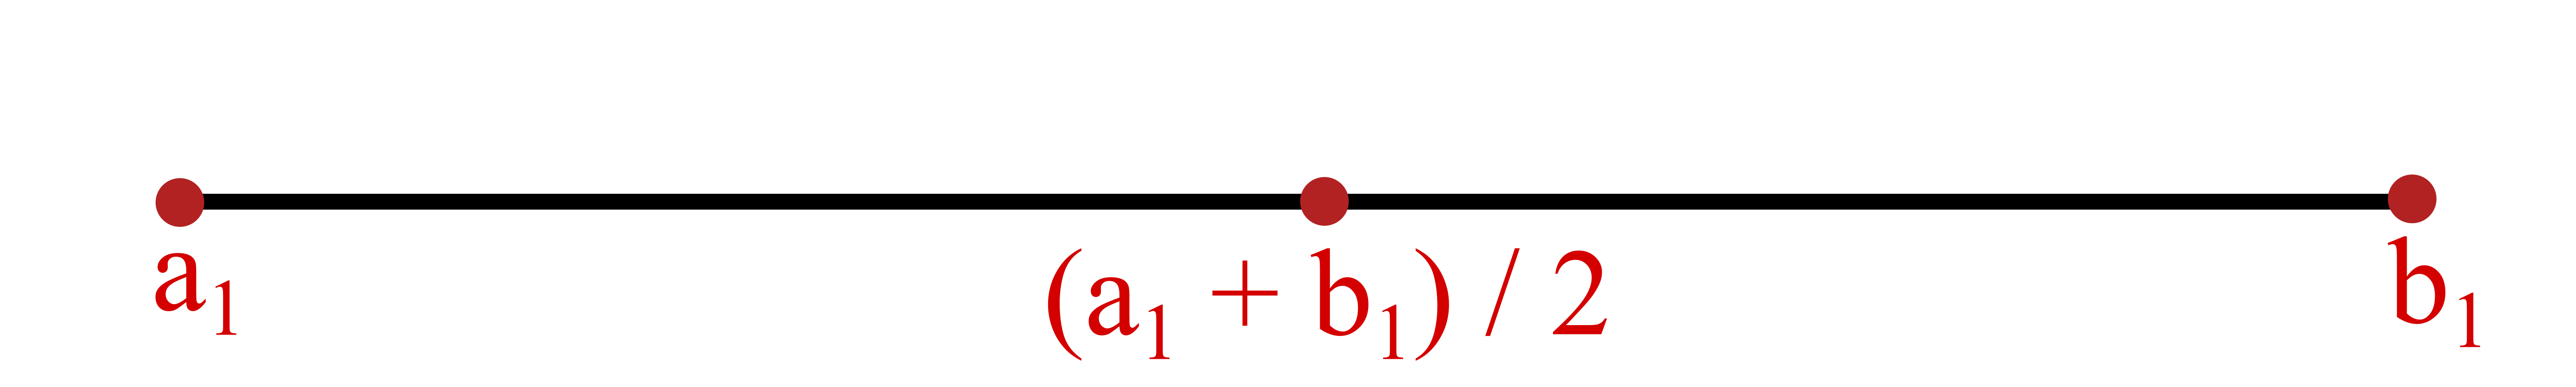
\includegraphics[width=0.8\textwidth]{veir1.png}
    \end{center}

    Поскольку все члены последовательности лежат в \([a_1, b_1]\), то либо в правой половине, либо в левой половине их бесконечно много. Если бы в каждой из них их было конечное число, то и внутри всего отрезка их было бы конечное число. В качестве \([a_2, b_2]\) выберем ту половину, которая содержит бесконечное количество членов последовательности. Тогда \(\exists n_2: n_1 < n_2, \; x_{n_2} \in [a_2, b_2]\). Снова делим отрезок пополам, снова в одной из половин бесконечное количество членов последовательности.

    \begin{center}
        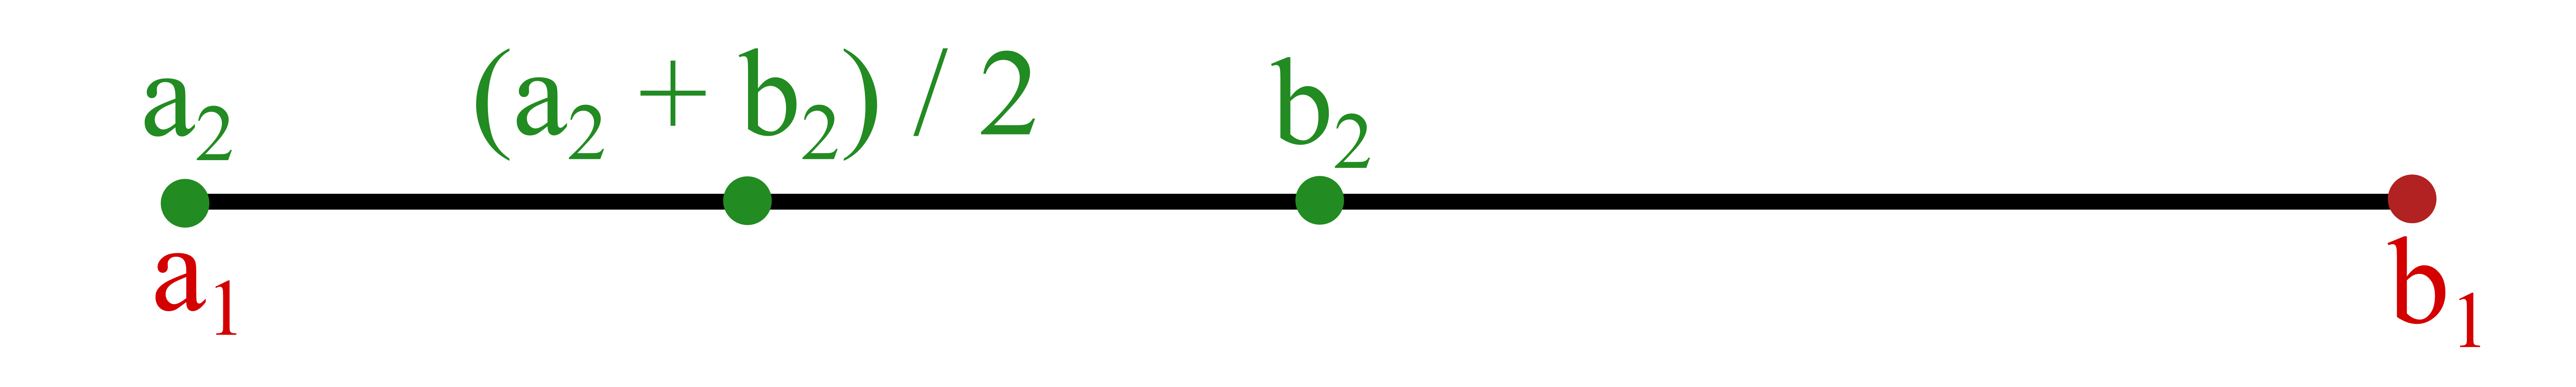
\includegraphics[width=0.8\textwidth]{veir2.png}
    \end{center}

    Назовем эту половинку \([a_3, b_3]\). Тогда снова получим, что \(\exists n_3: n_2 < n_3, \; x_{n_3} \in [a_3, b_3]\).

    \begin{center}
        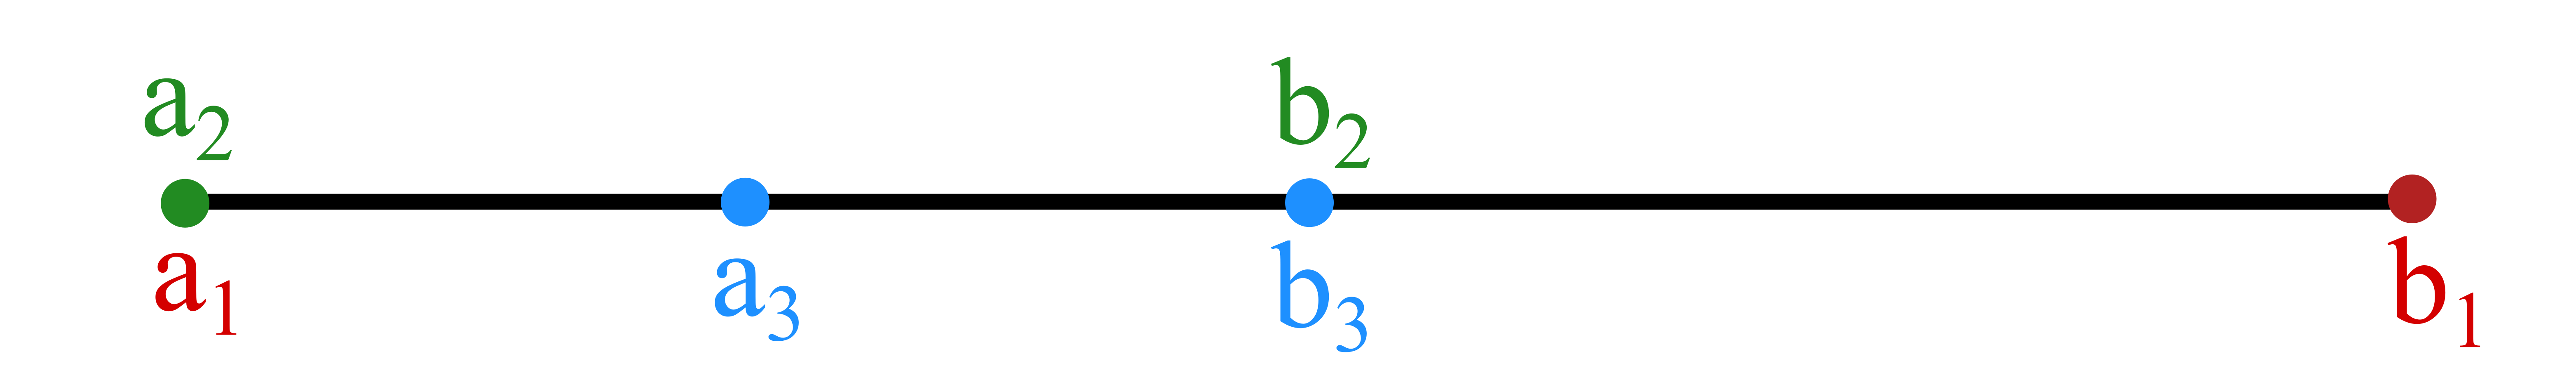
\includegraphics[width=0.8\textwidth]{veir3.png}
    \end{center}

    Продолжая повторять этот алгоритм, мы получим последовательность стягивающихся отрезков:
    \[
        [a_1, b_1] \supset [a_2, b_2] \supset [a_3, b_3] \supset \ldots
    \]

    Тогда длина отрезка \([a_k, b_k]\) равна:
    \[
        b_k - a_k = \frac{b_1 - a_1}{2^k} \overset{k \rightarrow \infty}{\longrightarrow} 0
    \]

    Кроме того, мы получили строго возрастающую последовательность индексов:
    \[
        n_1 < n_2 < n_3 < \ldots : x_{n_k} \in [a_k, b_k]
    \]

    Тогда по \plink{sec:Теорема Коши-Кантора о стягивающихся отрезках}{теореме о стягивающихся отрезках} \(\exists c: c \in \overset{\infty}{\underset{k = 1}{\bigcap}} [a_k, b_k]\) и \(\displaystyle c = \lim_{k \rightarrow \infty}{a_k} = \lim_{k \rightarrow \infty}{b_k}\).

    Так как \(x_{n_k} \in [a_k, b_k]\), то \(a_k \leq x_{n_k} \leq b_k\). Тогда по \plink{sub:Теорема о двух милиционерах}{теореме о двух милиционерах}:
    \[
        \begin{cases}
            a_k \rightarrow c \\
            b_k \rightarrow c \\
            a_k \leq x_{n_k} \leq b_k
        \end{cases}
        \implies
        x_{n_k} \rightarrow c
    \]

    Тогда \(\{x_n\}\) и будет той самой подпоследовательностью, имеющей предел.
\end{proof}

\section{Теорема Больцано-Коши}%
\label{sec:Теорема Больцано-Коши}

\begin{theorem}[Первая теорема Больцано-Коши]
    \newpar
    Пусть функция \(f(x)\) непрерывна на \([a, b]\) и значения \(f(a)\) и \(f(b)\) разных знаков. Тогда \(\exists c \in (a, b)\) для которой \(f(c) = 0\).
\end{theorem}

\begin{proof}
    Пусть \(f(a) < 0 < f(b)\). Случай при \(f(b) < 0 < f(a)\) доказывается аналогично.

    Если \(f(\dfrac{a + b}{2}) = 0\), то \(c = \dfrac{a + b}{2}\). Если это не так, то рассмотрим отрезок
    \[
        [a_1, b_1] =
        \begin{cases}
            \medskip
            [\dfrac{a + b}{2}, b], \text{ если } f(\dfrac{a + b}{2}) < 0 \\
            [a, \dfrac{a + b}{2}], \text{ если } f(\dfrac{a + b}{2}) > 0
        \end{cases}
    \]

    Тогда \(f(a_1) < 0 < f(b_1)\). Повторим алгоритм:
    Если \(f(\dfrac{a_1 + b_1}{2}) = 0\), то \(c = \dfrac{a_1 + b_1}{2}\). Если это не так, то рассмотрим отрезок
    \[
        [a_2, b_2] =
        \begin{cases}
            \medskip
            [\dfrac{a_1 + b_1}{2}, b_1], \text{ если } f(\dfrac{a_1 + b_1}{2}) < 0 \\
            [a_1, \dfrac{a_1 + b_1}{2}], \text{ если } f(\dfrac{a_1 + b_1}{2}) > 0
        \end{cases}
    \]

    Снова получим, что \(f(a_2) < 0 < f(b_2)\). Повторяя этот алгоритм снова и снова, мы получим последовательность вложенных отрезков:
    \[
        [a, b] \supset [a_1, b_1] \supset [a_2, b_2] \supset \ldots \supset [a_n, b_n] \supset \ldots
    \]

    Таких что \(f(a_n) < 0 < f(b_n)\). Причем длина \(n\)-го отрезка равна
    \[
        b_n - a_n = \frac{b - a}{2^n} \overset{n \to \infty}{\longrightarrow} 0
    \]

    Тогда по \plink{sec:Теорема Коши-Кантора о стягивающихся отрезках}{теореме о стягивающихся отрезках}:
    \[
        \exists c \in [a_n, b_n]: a_n \to c, b_n \to c
    \]

    Поскольку функция \(f(x)\) непрерывна в точке \(c\), значит, что, \(f(a_n) \to f(c)\) и \(f(b_n) \to f(c)\).

    Посмотрим на неравенство: \(f(a_n) < 0 < f(b_n)\). Исходя из предельного перехода в неравенствах получим, что \(f(c) \leq 0 \leq f(c)\). Следовательно \(f(c) = 0\).
\end{proof}

\begin{theorem}[Вторая теорема Больцано-Коши]
    \newpar
    Пусть \(f(x)\) непрерывна на \([a, b]\). Также пусть некоторое значение \(y\) лежит между \(f(a)\) и \(f(b)\). Тогда \(\exists c \in (a, b): f(c) = y\)
\end{theorem}

\begin{proof}
    Введем новую функцию \(g(x) = f(x) - y\). Поскольку функции \(f(x)\) и \(y\) непрерывны на \([a, b]\), то и \(g(x)\) непрерывна на \([a, b]\). Кроме того, поскольку \(y\) лежит между \(f(a)\) и \(f(b)\) значения функций \(g(a)\) и \(g(b)\) разных знаков. Тогда по теореме, доказанной выше:
    \[
        \exists c \in (a, b): g(c) = 0 \iff f(c) = y
    \]
\end{proof}

\begin{note}
    Эти теоремы доказывают следующее утверждение. Если непрерывная на отрезке функция принимает какие-то два значения, то она принимает и все значения, лежащие между ними.
\end{note}

\chapter{Пределы}%
\label{cha:Пределы}

\section{Вещественная ось. Бесконечность. Окрестность точки}%
\label{sec:Вещественная ось. Бесконечность. Окрестность точки}

\subsection{Вещественная ось}%
\label{sub:Вещественная ось}

\begin{siderules}
    \textbf{Вещественные} или \textbf{действительные} числа — это вместе взятые множества рациональных и иррациональных чисел. Множество вещественных чисел обозначается \(\mathbb{R}\) и часто называется \textbf{вещественной} или \textbf{числовой} прямой.
\end{siderules}

% TODO добавить аксиомы?

\subsection{Бесконечность}%
\label{sub:Бесконечность}

\begin{siderules}
    \textbf{Расширенная числовая прямая} \(\overbar{\mathbb{R}}\) — множество вещественных чисел, дополненное двумя элементами: \(+\infty\) (положительная бесконечность) и \(-\infty\) (отрицательная бесконечность), то есть:
    \[
        \overbar{\mathbb{R}} = \mathbb{R} \cup \{+\infty\} \cup \{-\infty\}
    \]
\end{siderules}

Бесконечности \(+\infty\) и \(-\infty\) не являются числами в обычном понимании этого слова. Их также называют \textbf{бесконечными числами}, в отличие от вещественных чисел \(a \in \mathbb{R}\), называемых \textbf{конечными числами}. При этом \(\forall x \in \mathbb{R}\) по определению полагают выполненными неравнества:
\[
    -\infty < x, \quad x < +\infty, \quad -\infty < +\infty
\]

\subsection{Окрестность точки}%
\label{sub:Окрестность точки}

\textbf{Окрестностью действительной точки} \(x_0\) называется любой открытый интервал, содержащий эту точку:
\[
    U(x_0) = \{x: -\varepsilon_1 < x - x_0 < \varepsilon_2; \varepsilon_1 > 0, \varepsilon_2 > 0\}
\]

\textbf{Эпсилон окрестностью точки} \(x_0\) называется множество точек, расстояние от которых до точки \(x_0\) меньше \(\varepsilon\):
\[
    U(x_0, \varepsilon) = \{x: |x - x_0| < \varepsilon\}
\]

\textbf{Проколотой окрестностью точки} \(x_0\) называется окрестность этой точки, из которой исключили саму эту точку \(x_0\):
\[
    \overset{\circ}{U}(x_0) = U(x_0) \; \backslash \; \{x_0\}
\]


\section{Определения предела функции. Односторонние пределы}%
\label{sec:Определения предела функции. Односторонние пределы}

\subsection{Предел функции по Коши}%
\label{sub:Предел функции по Коши}

Значение \(A\) называется \textbf{пределом} (\textbf{предельным значением}) функции \(f(x)\) в точке \(x_0\), если для любого положительного числа \(\varepsilon\) можно подобрать соответствующее ему положительное число \(\delta = \delta (\varepsilon)\) такое, что для всех аргументов \(x\), удовлетворяющих условию \(0 < |x - x_0| < \delta\), выполняется неравенство: \(0 \leq |f(x) - A| < \varepsilon\), то есть \(|f(x) -A| < \varepsilon\).

\begin{gather*}
    \lim_{x \to x_0}{f(x)} = A \iff \Big[ \forall \varepsilon > 0: \exists \delta = \delta (\varepsilon) > 0: (0 < |x - x_0| < \delta) \to (|f(x) - A| < \varepsilon) \Big]
\end{gather*}

\subsection{Окрестностное определение предела по Коши}
Значение \(A\) называется \textbf{пределом} (\textbf{предельным значением}) функции \(f(x)\) в точке \(x_0\), если для любой окрестности \(O(A)\) точки \(A\) существует проколотая окрестность \(\overset{\circ}{O}\) точки \(x_0\) такая, что образ этой окрестности \(f(\overset{\circ}{O}(x_0))\) лежит в \(O(A)\).

\begin{gather*}
    \lim_{x \to x_0}{f(x)} = A \iff \Big[ \forall O(A): \exists \overset{\circ}{O}(x_0): f(\overset{\circ}{O}(x_0) \subseteq O(A)) \Big]
\end{gather*}

\subsection{Определение предела по Гейне}%
\label{sub:Определение предела по Гейне}
Пусть функция \(f(x)\) определена в некоторой проколотой окрестности \(\overset{\circ}{U}(x_0)\) точки \(x_0\). Тогда значение \(A\) называется пределом функции \(f(x)\) при \(x \to x_0\), если для любой последовательности \(\{x_n\} \to x_0: x_n \in \overset{\circ}{U}(x_0)\) последовательность соответствующих значений \(\{f(x_n)\}\) стремится к \(A\):
\[
    \forall \{x_n\} \to x_0:\; x_n \in \overset{\circ}{U}(x_0) \implies \{f(x_n)\} \to A
\]

\subsection{Односторонние пределы. Бесконечный предел. Предел на бесконечности}%
\label{sub:Односторонние пределы. Бесконечный предел. Предел на бесконечности}

\begin{siderules}
    Под односторонним пределом числовой функции подразумевают приближение к предельной точки с одной стороны (справа или слева).
\end{siderules}

\begin{definition}[Левый предел]
    Пусть \(x \to x_0\), \(\forall x \; x < x_0\), \((f(x) - A) \to 0\). Тогда число \(A\) называется пределом функции \(f(x)\) в точке \(x_0\) \textbf{слева} и записывается как:
    \[
        \lim_{x \to x_0 - 0}{f(x)}
    \]
\end{definition}

\begin{definition}[Правый предел]
    Пусть \(x \to x_0\), \(\forall x \; x > x_0\), \((f(x) - A) \to 0\). Тогда число \(A\) называется пределом функции \(f(x)\) в точке \(x_0\) \textbf{справа} и записывается как:
    \[
        \lim_{x \to x_0 + 0}{f(x)}
    \]
\end{definition}

\begin{note}
    Для существования двустороннего предела функции необходимо и достаточно, чтобы оба односторонних предела существовали и равнялись между собой. Верно и обратное.
\end{note}

\begin{definition}[Бесконечный предел]
    Пусть функция \(f(x)\) определена в некоторой проколотой окрестности точки \(x_0\). Говорят, что ее предел в этой точке равен бесконечности, если:
    \[
        \lim_{x \to x_0}{f(x)} = \infty \iff \forall M > 0 \; \exists \delta_M > 0: (0 < |x - x_0| < \delta_M) \implies (|f(x)| > M)
    \]
\end{definition}

\begin{definition}[Предел на бесконечности]
    Число \(A\) называется пределом функции \(f(x)\) на бесконечности (или при \(x \to \infty\)), если:
    \[
        \lim_{x \to \infty}{f(x)} = A \iff \forall \varepsilon > 0 \; \exists \delta_{\varepsilon} > 0: \forall x \in D(f): |x| > \delta_{\varepsilon} \implies (|f(x) - A| < \varepsilon)
    \]
\end{definition}

\section{Бесконечно малые и бесконечно большие функции}%
\label{sec:Бесконечно малые функции и их свойства}

\subsection{Бесконечно малые функции и их свойства}%
\label{sub:Бесконечно малые функции и их свойства}

\begin{definition}
    Функция \(\alpha(x)\) называется \textbf{бесконечно малой} при \(x \to x_0\), если \(\displaystyle \exists \lim_{x \to x_0}{\alpha(x)}\) и \(\displaystyle \lim_{x \to x_0}{\alpha(x)} = 0\).
\end{definition}

\subsection{Свойства бесконечно малых функций}

\begin{property}
    \newpar
    Пусть есть бесконечно малая функция \(\alpha(x)\) при \(x \to x_0\). Также есть функция \(g(x)\), ограниченная в некоторой проколотой окрестности \(\overset{\circ}{U}_g(x_0)\). Тогда их произведение есть бесконечно малая функция:
    \[
        \lim_{x \to x_0}{(\alpha(x) \cdot g(x))} = 0
    \]
\end{property}

\begin{proof}
    Так как \(g(x)\) ограничена в \(\overset{\circ}{U}_g(x_0)\), то \(\exists M: \forall x \in \overset{\circ}{U}_g(x_0) \implies |g(x)| \leq M\).

    Если \(\displaystyle \exists \lim_{x \to x_0}{\alpha(x)}\), то \(\exists \overset{\circ}{U}_\alpha (x_0)\), на которой определена функция \(\alpha(x)\).

    Тогда \(\forall \varepsilon > 0: x \in \overset{\circ}{U}_\alpha(x_0) \implies |\alpha(x)| < \dfrac{\varepsilon}{M}\).

    Пусть \(\overset{\circ}{U}(x_0) = \min(\overset{\circ}{U}_\alpha(x_0), \overset{\circ}{U}_g(x_0))\).

    Тогда
    \[
        \forall \varepsilon > 0: x \in \overset{\circ}{U}(x_0) \implies |\alpha(x) \cdot g(x)| \leq |\alpha(x)| \cdot |g(x)| < \dfrac{\varepsilon}{M} \cdot M = \varepsilon
    \]


    Следовательно:
    \[
        \lim_{x \to x_0}{(\alpha(x) \cdot g(x))} = 0
    \]
\end{proof}

\begin{note}
    Из этого свойства следует, что произведение б. м. ф. на число есть функция бесконечно малая.
\end{note}

\begin{property}
    \newpar
    Пусть \(\alpha(x)\) и \(\beta(x)\) — бесконечно малые функции при \(x \to x_0\). Тогда их \textbf{сумма}, \textbf{разность} и \textbf{произведение} являются также бесконечно малыми функциями при \(x \to x_0\).
\end{property}

\begin{proof}
    Докажем, что сумма бесконечно малых функций являетсяя бесконечно малой функцией. Разность и произведение доказываются аналогично.

    \(\alpha(x)\) б. м. ф. \(\implies \alpha(x)\) определена в некоторой окрестности \(\overset{\circ}{U}_\alpha(x_0)\)

    Тогда \(\forall \varepsilon > 0: x \in \overset{\circ}{U}_\alpha(x_0) \implies |\alpha(x)| < \dfrac{\varepsilon}{2}\)

    \(\beta(x)\) б. м. ф. \(\implies \beta(x)\) определена в некоторой окрестности \(\overset{\circ}{U}_\beta(x_0)\).

    Тогда \(\forall \varepsilon > 0: x \in \overset{\circ}{U}_\beta(x_0) \implies |\beta(x)| < \dfrac{\varepsilon}{2}\)

    Пусть \(\overset{\circ}{U}(x_0) = \min(\overset{\circ}{U}_\alpha(x_0), \overset{\circ}{U}_\beta(x_0))\)

    Тогда \(\forall \varepsilon > 0: x \in \overset{\circ}{U}(x_0) \implies |\alpha(x) + \beta(x)| < |\alpha(x)| + |\beta(x)| < \dfrac{\varepsilon}{2} + \dfrac{\varepsilon}{2} = \varepsilon\)

    Следовательно:
    \[
        \lim_{x \to x_0}{(\alpha(x) + \beta(x))} = 0
    \]
\end{proof}

\begin{theorem*}[о частном от деления ограниченной снизу функции на бесконечно малую]
    Пусть есть бесконечно малая функция \(\alpha(x)\) при \(x \to x_0\), которая определена в некоторой проколотой окрестности \(\overset{\circ}{U}_{\alpha}(x_0): \forall x \in \overset{\circ}{U}(x_0) \alpha(x) \neq 0\). Также есть функция \(g(x)\), которая определена и ограниченна в некоторой проколотой окрестности \(\overset{\circ}{U}_{g}(x_0)\) точки \(x_0\) числом \(M\): \(0 < |g(x)| \leq M\). Тогда их частное есть бесконечно большая функция:
    \[
        \lim_{x \to x_0}{\frac{g(x)}{\alpha(x)}} = \infty
    \]
\end{theorem*}
% TODO добавить доказательство

\subsection{Бесконечно большие функции и их свойства}%
\label{sec:Бесконечно большие функции и их свойства}

\begin{definition}
    Функция \(f(x)\) называется \textbf{бесконечно большой} при \(x \to x_0\), если \(\displaystyle \exists \lim_{x \to x_0}{f(x)}\) и \(\displaystyle \lim_{x \to x_0}{f(x)} = \infty\).
\end{definition}

\begin{theorem*}[о сумме ограниченной функции и бесконечно большой]
    \newpar
    \textbf{Сумма} или \textbf{разность} ограниченной функции на некоторой проколотой окрестности точки \(x_0\) и бесконечно большой функции при \(x \to x_0\) является бесконечно большой функцией при \(x \to x_0\).
\end{theorem*}
% TODO добавить доказательство

\begin{theorem*}[о произведении ограниченной снизу функции на бесконечно большую функцию]
    \newpar
    Пусть есть функция \(f(x)\) является бесконечно большой при \(x \to x_0\). Также есть функция \(g(x)\), которая определена на некоторой проколотой окрестности \(\overset{\circ}{O}(x_0)\) точки \(x_0\) и ограничена снизу значением \(M: 0 < M \leq |g(x)|\). Тогда их произведение является бесконечно большой функцией при \(x \to x_0\):
    \[
        \lim_{x \to x_0}{(f(x) \cdot g(x))} = \infty
    \]
\end{theorem*}
% TODO добавить доказательство

\begin{theorem*}[о частном от деления ограниченной функции на бесконечно большую]
    Пусть есть функция \(f(x)\) является бесконечно большой при \(x \to x_0\). Также есть функция \(g(x)\), ограниченная на некоторой проколотой окрестности \(\overset{\circ}{U_g}(x_0)\) точки \(x_0\). Тогда
    \[
        \lim_{x \to x_0}{\dfrac{g(x)}{f(x)}} = 0
    \]
\end{theorem*}
% TODO добавить доказательство

\subsection{Связь между бесконечно большими и бесконечно малыми функциями}
\label{sec:Связь между бесконечно большими и бесконечно малыми функциями}
\begin{itemize}
    \item {Если функция \(f(x)\) является бесконечно большой при \(x \to x_0\), то функция \(\dfrac{1}{f(x)}\) является бесконечно малой при \(x \to x_0\).}
    \item {Если функция \(\alpha(x)\)} является бесконенчо малой при \(x \to x_0\) и \(\alpha(x) \neq 0\), то функция \(\dfrac{1}{\alpha(x)}\) является бесконечно большой при \(x \to x_0\).
\end{itemize}

Связь между бесконечно малой и бесконечно большой функцией можно выразить символическим образом:
\[
    \frac{1}{\infty} = 0 \hspace{1cm} \frac{1}{0} = \infty
\]
Следовательно:
\begin{gather*}
    \frac{1}{+0} = +\infty \hspace{1cm} \frac{1}{-0} = -\infty \\
    \frac{1}{+ \infty} = +0 \hspace{1cm} \frac{1}{-\infty} = -0
\end{gather*}

\subsection{Арифметические свойства}%
\label{sub:Арифметические свойства}

Пусть существуют пределы функций:
\begin{gather*}
    \lim_{x \to x_0}{g(x)} = a \neq \infty \\
    \lim_{x \to x_0}{y(x)} = b \neq 0 \\
    \lim_{x \to x_0}{\alpha(x)} = 0 \\
    \lim_{x \to x_0}{f(x)} = \infty
\end{gather*}

Тогда функция \(\alpha(x)\) является бесконечно малой при \(x \to x_0\), а функция \(f(x)\) — бесконечно большой при \(x \to x_0\).
\begin{gather*}
    \lim_{x \to x_0}{(g(x) \pm f(x))} = \infty \\
    \lim_{x \to x_0}{(g(x) \cdot \alpha(x))} = 0 \\
    \lim_{x \to x_0}{(y(x) \cdot f(x))} = \infty \\
    \lim_{x \to x_0}{\frac{g(x)}{f(x)}} = 0 \\
    \lim_{x \to x_0}{\frac{y(x)}{\alpha(x)}} = \infty
\end{gather*}

\section{Алгебра о-малых}%
\label{sec:Алгебра о-малых}

\begin{gather*}
    \lim_{x \to 0}{o(1)} = 0 \\
    o(x) \cdot o(x) = o(x_2) \\
    o(x) + o(x) = o(x) \\
    o(f(x)) = f(x) \cdot o(1) \\
    o(x) = x \cdot o(1)
\end{gather*}

\begin{proof}
    \begin{gather*}
        \lim_{x \to x_0}{\dfrac{o(x) \cdot o(x)}{x^2}} = \lim_{x \to 0}{\dfrac{o(x)}{x}} \cdot \lim_{x \to 0}{\dfrac{o(x)}{x}} = 0 \\
        \lim_{x \to x_0}{\dfrac{o(x) + o(x)}{x}} = \lim_{x \to x_0}{\dfrac{o(x)}{x}} + \lim_{x \to x_0}{\dfrac{o(x)}{x}} = 0 \\
        \lim_{x \to 0}{\dfrac{o(f(x))}{f(x)}} = 0 \implies \frac{o(f(x))}{f(x)} = o(1)
    \end{gather*}
\end{proof}

\section{Сравнение бесконечно малых. Эквивалентные функции}%
\label{sec:Сравнение бесконечно малых. Эквивалентные функции}

\begin{siderules}
    Пусть функции \(\alpha(x)\) и \(\beta(x)\) являются бесконечно малыми функциями в точке \(x = x_0\). Также пусть:
    \[
        \lim_{x \to x_0}{\dfrac{\alpha(x)}{\beta(x)}} = q
    \]

    Тогда, если:
    \begin{itemize}
        \item {\(q\) — это конечное, отличное от нуля число, то \(\alpha(x)\) и \(\beta(x)\) — \textbf{бесконечно малые одного порядка}.}
        \item {\(q = 0\), то \(\alpha(x)\) называется \textbf{бесконечно малой функцией более высокого порядка}, чем функция \(\beta(x)\).}
        \item {\(q = \infty\), то функция \(\alpha(x)\) называется \textbf{бесконечно малой функцией более низкого порядка}, чем функция \(\beta(x)\).}
        \item {\(q = 1\), то \(\alpha(x)\) и \(\beta(x)\) — \textbf{эквивалентные бесконечно малые функции}, то есть \(\alpha(x) \sim \beta(x)\).}
    \end{itemize}
\end{siderules}

\begin{theorem}[Связь эквивалентный функций с \(o\) малым]
    \newpar
    Для того, чтобы две функции \(f(x)\) и \(g(x)\) были эквивалентными, необходимо и достаточно, чтобы при \(x \to x_0\) выполнялось условие:
    \[
        f(x) = g(x) + o(g(x))
    \]
\end{theorem}

\begin{proof}
    \begin{gather*}
        \frac{f(x)}{g(x)} = 1 + o(1) \implies f(x) = g(x) + o(1) \cdot g(x) = g(x) + o(g(x)) \\
        \frac{f(x)}{g(x)} = 1 + \frac{o(g(x))}{g(x)} = 1 + o(1) \implies \lim_{x \to x_0}{\dfrac{f(x)}{g(x)}} = 1
    \end{gather*}
\end{proof}

\begin{theorem}[Замена бесконечно малой на эквивалентную]
    \newpar
    Пусть функции \(f(x)\) и \(g(x)\) бесконечно малые при \(x \to x_0\) и
    \[
        \begin{cases}
            f(x) \sim f_1(x) \\
            \smallskip
            g(x) \sim g_1(x) \\
            \displaystyle \lim_{x \to x_0}{\dfrac{f_1(x)}{g_1(x)}} = A
        \end{cases}
    \]
    Тогда
    \[
        \lim_{x \to x_0}{\dfrac{f_(x)}{g_(x)}} = A
    \]
\end{theorem}

\begin{proof}
    \[
        \lim_{x \to x_0}{\dfrac{f(x)}{g(x)}} = \lim_{x \to x_0}{\Big(\dfrac{f(x)}{f_1(x)} \cdot \dfrac{f_1(x)}{g_1(x)} \cdot \dfrac{g_1(x)}{g(x)}\Big)} = A
    \]

    Поскольку
    \[
        \begin{cases}
            \smallskip
            \displaystyle \lim_{x \to x_0}{\frac{f(x)}{f_1(x)}} = 1 \\
            \displaystyle \lim_{x \to x_0}{\frac{g_1(x)}{g(x)}} = 1
        \end{cases}
    \]
\end{proof}

\section{Основные теоремы о пределах}%
\label{sec:Основные теоремы о пределах}

\begin{theorem}[Предельный переход в равенстве]
    Если две функции принимают одинаковые значения в окрестности некоторой точки, то их пределы в этой точке совпадают.
    \[
        \forall x \in \overset{\circ}{U}(x_0) \rightarrow f(x) = g(x) \implies \lim_{x \to x_0}{f(x)} = \lim_{x \to x_0}{g(x)}
    \]
\end{theorem}

\begin{theorem}[Предельный переход в неравенстве]
    Если значения функции \(f(x)\) в окрестности некоторой точки не превосходят соответствующих значений функции \(g(x)\), то предел функции \(f(x)\) в этой точке не превосходит предела функции \(g(x)\).
    \[
        \forall x \in \overset{\circ}{U}(x_0) \; f(x) \leq g(x) \implies \lim_{x \to x_0}{f(x)} \leq \lim_{x \to x_0}{g(x)}
    \]
\end{theorem}

\begin{theorem}
    Предел константы равен самой константе
    \[
        \lim_{x \to x_0}{c} = c, \quad c = const
    \]
\end{theorem}

\begin{proof}
    Пусть \(\forall x \in D \; f(x) = c\).
    Воспользуемся определением предела функции по Коши:
    \[
        \forall \varepsilon > 0: \; \exists \delta = \delta(\varepsilon) > 0: (0 < |x - x_0| < \delta) \rightarrow (|f(x) - A| < \varepsilon)
    \]

    Тогда
    \[
        \forall x \in D \quad |f(x) - A| = |c - c| = 0 \quad \implies \quad \forall x \in D \quad |f(x) - A | < \varepsilon
    \]

    Следовательно
    \[
        \lim_{x \to x_0}{c} = c
    \]
\end{proof}

\begin{theorem}
    Функция не может иметь двух различных пределов в одной точке.
\end{theorem}

\begin{proof}
    Будем доказывать от противного.

    Пусть:
    \[
        \begin{cases}
            \displaystyle
            \lim_{x \to x_0}{f(x)} = A \\
            \displaystyle
            \lim_{x \to x_0}{f(x)} = B \\
            A \neq B
        \end{cases}
    \]

    Тогда по \plink{theorem:Теорема о связи функции, ее предела и бесконечно малой функции}{теореме о связи предела и бесконечно малой функции}:
    \[
        \begin{cases}
            f(x) - A = \alpha(x) \text{ — б. м. при } x \to x_0 \\
            f(x) - B = \beta(x) \text{ — б. м. при } x \to x_0
        \end{cases}
    \]

    Вычитая эти равенства, получим:
    \[
        B - A = \alpha(x) - \beta(x)
    \]

    Тогда, переходя к пределам:
    \begin{gather*}
        \lim_{x \to x_0}{(B - A)} = \lim_{x \to x_0}{(\alpha(x) - \beta(x))} \\
        \lim_{x \to x_0}{(B - A)} = 0 \\
        B - A = 0 \\
        B = A
    \end{gather*}

    Получили противоречие \(B = A\) и \(B \neq A\).
\end{proof}

\begin{theorem}
    Если каждое слагаемое алгебраической суммы функций имеет предел при \(x \to x_0\), и алгебраическая сумма имеет предел при \(x \to x_0\), причем предел алгебраической суммы равен алгебраической сумме пределов.
    \[
        \lim_{x \to x_0}{(f(x) + g(x) - h(x))} = \lim_{x \to x_0}{f(x)} + \lim_{x \to x_0}{g(x)} - \lim_{x \to x_0}{h(x)}
    \]
\end{theorem}

\begin{proof}
    Пусть:
    \[
        \begin{cases}
            \displaystyle
            \lim_{x \to x_0}{f(x)} = A \\
            \displaystyle
            \lim_{x \to x_0}{g(x)} = B \\
            \displaystyle
            \lim_{x \to x_0}{h(x)} = C
        \end{cases}
    \]

    Тогда \plink{theorem:Теорема о связи функции, ее предела и бесконечно малой функции}{по теореме о связи предела и бесконечно малой функции:}
    \[
        \begin{cases}
            f(x) - A = \alpha(x) \\
            g(x) - B = \beta(x)  \\
            h(x) - C = \gamma(x) \\
        \end{cases}
    \]

    где \(\alpha(x)\), \(\beta(x)\), \(\gamma(x)\) — б. м. при \(x \to x_0\). Тогда:

    \[
        f(x) + g(x) - h(x) - (A + B - C) = \alpha(x) + \beta(x) - \gamma(x)
    \]

    Переходя к пределам:
    \[
        \lim_{x \to x_0}{(f(x) + g(x) - h(x))} = A + B - C = \lim_{x \to x_0}{f(x)} + \lim_{x \to x_0}{g(x)} - \lim_{x \to x_0}{h(x)}
    \]
\end{proof}

\begin{theorem}
    Если каждый из сомножителей произведения конечного числа функций имеет предел \(x \to x_0\), то и произведение имеет предел при \(x \to x_0\), причем предел произведения равен произведению пределов.
    \[
        \lim_{x \to x_0}{(f(x) \cdot g(x))} = \lim_{x \to x_0}{f(x)} \cdot \lim_{x \to x_0}{g(x)}
    \]
\end{theorem}

\begin{proof}
    Пусть:
    \[
        \begin{cases}
            \displaystyle
            \lim_{x \to x_0}{f(x)} = A \\
            \displaystyle
            \lim_{x \to x_0}{g(x)} = B
        \end{cases}
    \]

    Тогда \plink{theorem:Теорема о связи функции, ее предела и бесконечно малой функции}{по теореме о связи предела и бесконечно малой функции:}
    \[
        \begin{cases}
            f(x) = A + \alpha(x) \\
            g(x) = B + \beta(x)
        \end{cases}
    \]

    где \(\alpha(x)\), \(\beta(x)\) — б. м. при \(x \to x_0\). Тогда:

    \begin{gather*}
        f(x) \cdot g(x) = (A + \alpha(x)) \cdot (B + \beta(x)) \\
        f(x) \cdot g(x) = AB + \underbrace{A \beta(x) + \alpha(x) B + \alpha(x) + \beta(x)}_{\text{бесконечно малые}}
    \end{gather*}

    Переходя к пределам:
    \[
        \lim_{x \to x_0}{(f(x) \cdot g(x))} = AB =  \lim_{x \to x_0}{f(x)} \cdot \lim_{x \to x_0}{g(x)}
    \]
\end{proof}

\begin{consequence}
    Постоянный множитель можно выносить за знак предела.
    \[
        \lim_{x \to x_0}{(c \cdot f(x))} = c \cdot \lim_{x \to x_0}{f(x)}
    \]
\end{consequence}

\begin{theorem}
    Если функции \(f(x)\) и \(g(x)\) имеют придел при \(x \to x_0\), причем \(\displaystyle \lim_{x \to x_0}{g(x)} \neq 0\), то их частное имеет предел при \(x \to x_0\), причем предел частного равен частном пределов.
    \[
        \lim_{x \to x_0}{\frac{f(x)}{g(x)}} = \frac{\displaystyle \lim_{x \to x_0}{f(x)}}{\displaystyle \lim_{x \to x_0}{g(x)}}, \quad \lim_{x \to x_0}{g(x)} \neq 0
    \]
\end{theorem}

\begin{proof}
    Пусть:
    \[
        \begin{cases}
            \displaystyle
            \lim_{x \to x_0}{f(x)} = A \\
            \displaystyle
            \lim_{x \to x_0}{g(x)} = B
        \end{cases}
    \]

    Тогда \plink{theorem:Теорема о связи функции, ее предела и бесконечно малой функции}{по теореме о связи предела и бесконечно малой функции:}
    \[
        \begin{cases}
            f(x) = A + \alpha(x) \\
            g(x) = B + \beta(x)
        \end{cases}
    \]

    где \(\alpha(x)\), \(\beta(x)\) — б. м. при \(x \to x_0\). Тогда:

    \begin{gather*}
        \frac{f(x)}{g(x)} = \frac{A + \alpha(x)}{B + \beta(x)} \\
        \frac{f(x)}{g(x)} = \frac{A + \alpha(x)}{B + \beta(x)} + \frac{A}{B} - \frac{A}{B} \\
        \frac{f(x)}{g(x)} = \frac{A}{B} + \underbrace{\frac{B\alpha(x) - A \beta(x)}{B(B + \beta(x))}}_{\text{бесконечно малая}}
    \end{gather*}

    Переходя к пределам:
    \[
        \lim_{x \to x_0}{\dfrac{f(x)}{g(x)}} = \frac{A}{B} = \dfrac{\displaystyle \lim_{x \to x_0}{f(x)}}{\displaystyle \lim_{x \to x_0}{g(x)}}
    \]
\end{proof}

% TODO переместить в другое место
\begin{theorem}[Связь функции, ее предела и бесконечно малой функции]
    \label{theorem:Теорема о связи функции, ее предела и бесконечно малой функции}
    \newpar

    Если функция \(f(x)\) имеет предел \(\displaystyle \lim_{x \to x_0}{f(x)} = A\), то разность между функцией и значением предела есть функция, бесконечно малая при \(x \to x_0\).
    \[
        \lim_{x \to x_0}{f(x)} = A \quad \iff \quad f(x) - A = \alpha(x), \quad \lim_{x \to x_0}{\alpha(x)} = 0
    \]
\end{theorem}

\begin{proof}
    Для функции \(f(x)\) воспользуемся определением предела по Коши:
    \[
        \lim_{x \to x_0}{f(x)} = A \; \implies \quad \forall \varepsilon > 0 \quad \exists \delta > 0: (0 < |x - x_0| < \delta) \rightarrow (|f(x) - A| < \varepsilon)
    \]

    В случае бесконечно малой функции определение выглядит так:
    \[
        \lim_{x \to x_0}{\alpha(x)} = 0 \; \implies \quad \forall \varepsilon > 0 \quad \exists \delta > 0: (0 < |x - x_0| < \delta) \rightarrow (|\alpha(x)| < \varepsilon)
    \]

    Сравнивая определения пределов функций, видим, что \(f(x) - A = \alpha(x)\).
\end{proof}

\section{Сравнение пределов. Теорема о двух милиционерах}%
\label{sec:Сравнение пределов. Теорема о двух милиционерах}

\subsection{Теорема о двух милиционерах}%
\label{sub:Теорема о двух милиционерах}
\begin{theorem}
    Пусть есть 3 вещественные последовательности \((x_n), (y_n), (z_n)\), такие что
    \begin{gather*}
        \begin{cases}
            \forall n \;\; x_n \leq y_n \leq z_n        \\
            \displaystyle{\lim_{n \to \infty}{x_n}} = a \\
            \displaystyle{\lim_{n \to \infty}{z_n}} = a
        \end{cases}
    \end{gather*}

    Тогда \(\exists \displaystyle{\lim_{n \to \infty}{y_n}}\) и  \(\displaystyle{\lim_{n \to \infty}{y_n}} = a\).
\end{theorem}

\begin{proof}
    \(
    \forall \varepsilon > 0 \;\; \exists N_1: \;\; \forall n > N_1 \rightarrow |x_n - a| < \varepsilon \implies a - \varepsilon < x_n
    \)

    \(
    \forall \varepsilon > 0 \;\; \exists N_2: \;\; \forall n > N_2 \rightarrow |z_n - a| < \varepsilon \implies z_n < a + \varepsilon
    \)

    \(N = \max(N_1, N_2)\)

    \medskip

    \(\forall n > N\)

    \(a - \varepsilon < x_n \leq y_n \leq z_n < a + \varepsilon\)

    \(a - \varepsilon < y_n < a + \varepsilon \implies \exists \displaystyle{\lim_{n \to \infty}{y_n}} \text{ и } \displaystyle{\lim_{n \to \infty}{y_n}} = a\)
\end{proof}

\section{Первый замечательный предел}\label{sec:limit_1}
\begin{gather*}
    \lim_{x \to 0}{\frac{\sin{x}}{x}} = 1
\end{gather*}

Рассмотрим односторонние пределы \(\displaystyle{\lim_{x \to +0}{\dfrac{\sin{x}}{x}}}\) и \(\displaystyle{\lim_{x \to -0}{\dfrac{\sin{x}}{x}}}\) и докажем, что они равны \(1\).

Рассмотрим случай \(x \in \Big(0; \dfrac{\pi}{2}\Big)\).
Отложим этот угол на единичной окружности так, чтобы его вершина совпадала с началом координат, а одна сторона совпадала с осью \(OX\).
Пусть \(K\) — точка пересечения второй сторны угла с единичной окружностью, а точка \(L\) — с касательной к этой окружност в точке \(A = (1; 0)\). Точка \(H\) — проекция точки \(K\) на ось \(OX\).

\begin{center}
    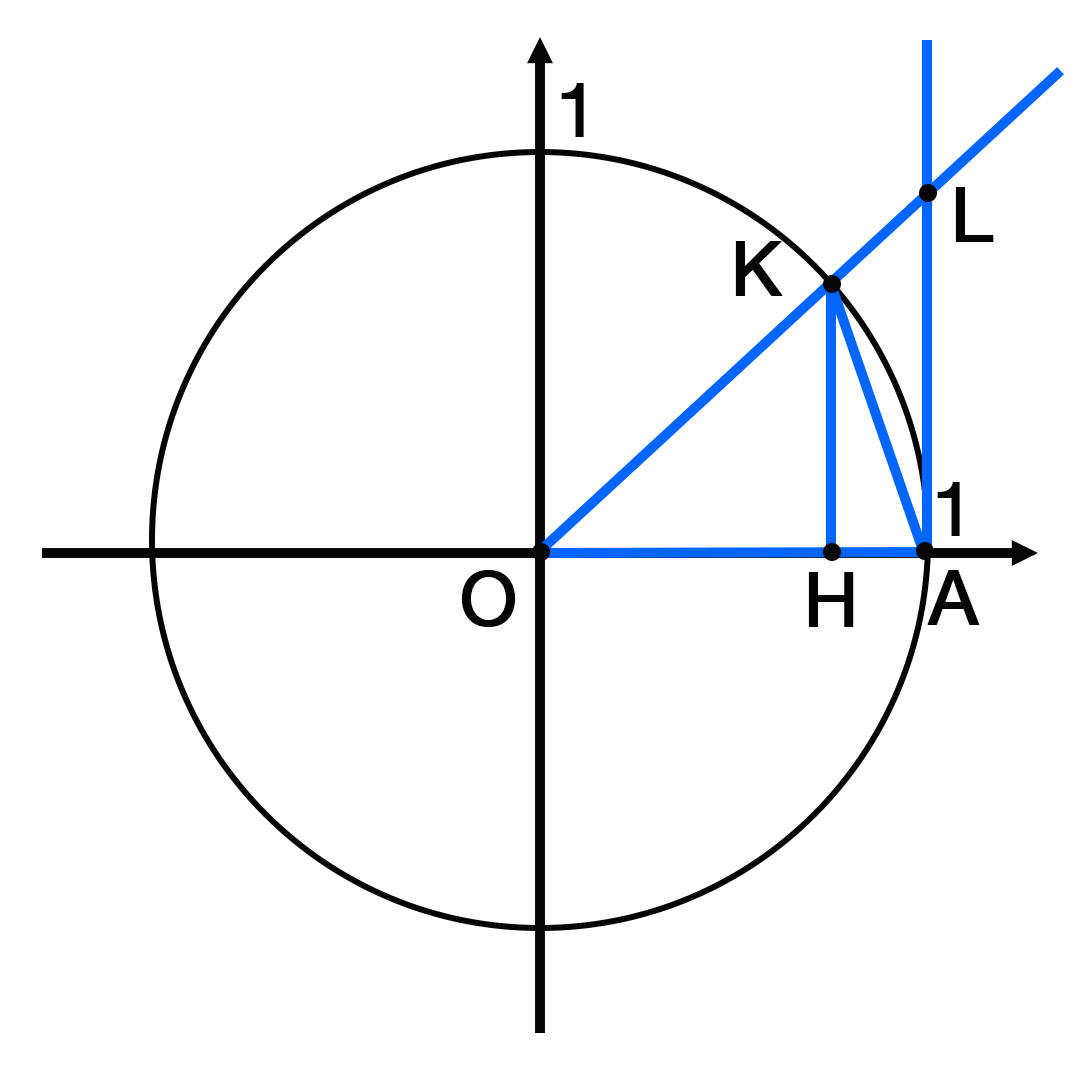
\includegraphics[width=0.6\textwidth]{limit_1.png}
\end{center}

Очевидно, что \(S_{\triangle OKA} < S_{sect KOA} < S_{\triangle OAL}\), где \(S_{sect KOA}\) — площадь сектора  \(KOA\). Поскольку \(|KH| = \sin{x}, |LA| = \tg{x}\):
\begin{gather*}
    S_{\triangle OKA} = \frac{1}{2} \cdot |OA| \cdot |KH| = \frac{1}{2} \cdot 1 \cdot \sin{x} = \frac{\sin{x}}{2} \\
    S_{sect KOA} = \frac{1}{2} \cdot |OA|^2 \cdot x = \frac{x}{2}                                                 \\
    S_{\triangle OAL} = \frac{1}{2} \cdot |OA| \cdot |LA| = \frac{\tg{x}}{2}
\end{gather*}
Тогда, заменив площади в неравенстве, получим:
\begin{gather*}
    \dfrac{\sin{x}}{2} < \dfrac{x}{2} < \dfrac{\tg{x}}{2}
\end{gather*}

Так как при \(x \to +0: \sin{x} > 0, x > 0, \tg{x} > 0\), получим:
\begin{gather*}
    \dfrac{1}{\tg{x}} < \dfrac{1}{x} < \dfrac{1}{\sin{x}} \iff \cos{x} < \dfrac{\sin{x}}{x} < 1
\end{gather*}

Перейдем к пределу:
\begin{gather*}
    \lim_{x \to +0}{\cos{x}} \leq \lim_{x \to +0}{\dfrac{\sin{x}}{x}} \leq 1 \implies 1 \leq \lim_{x \to +0}{\dfrac{\sin{x}}{x}} \leq 1 \implies \lim_{x \to +0}{\dfrac{\sin{x}}{x}} = 1
\end{gather*}

Найдем левый односторонний предел. Пусть \(t = -x \implies t \to +0\):
\begin{gather*}
    \lim_{x \to -0}{\dfrac{\sin{x}}{x}} = \lim_{t \to +0}{\dfrac{\sin{(-t)}}{-t}} = \lim_{t \to +0}{\dfrac{-\sin{t}}{-t}} = \lim_{t \to +0}{\dfrac{\sin{t}}{t}} = 1
\end{gather*}

Правый и левый односторонний пределы существуют и равны \(1\), следовательно и сам предел равен 1.

\subsubsection{Следствия}
\begin{enumerate}
    \item {\(\lim_{x \to 0}{\dfrac{\tg{x}}{x}} = 1\)}
    \item {\(\lim_{x \to 0}{\dfrac{\arcsin{x}}{x}} = 1\)}
    \item {\(\lim_{x \to 0}{\dfrac{\arctg{x}}{x}} = 1\)}
    \item {\(\lim_{x \to 0}{\dfrac{1 - \cos{x}}{\frac{x^2}{2}}} = 1\)}
\end{enumerate}

\section{Второй замечательный предел. Число \(e\)}\label{sec:limit_2}
\begin{gather*}
    \lim_{x \to \infty}{\Big(1 + \frac{1}{x}\Big)^x} = e \text{ или } \lim_{x \to 0}{(1 + x)^\frac{1}{x}} = e
\end{gather*}

\begin{proof}
    Сначала докажем теорему для натуральных значений \(x\):
    \begin{gather*}
        x_n = \Big(1 + \frac{1}{n}\Big)^n; n \in \mathbb{N}
    \end{gather*}

    По формуле бинома Ньютона:
    \begin{align*}
        (a + b)^n & = a^n + \frac{n}{1} \cdot a^{n - 1} + \frac{n(n - 1)}{1 \cdot 2} \cdot a^{n - 2} \cdot b^2 + ... + \\
                  & + \frac{n(n - 1)(n - 2)...(n - (n - 1))}{1 \cdot 2 \cdot 3 \cdot ... \cdot n} \cdot b^n
    \end{align*}

    Полагая \(a = 1, b = \dfrac{1}{n}\), получим:
    \begin{align*}
        \Big(1 + \frac{1}{n}\Big)^n & = 1 + \frac{n}{1} \cdot \frac{1}{n} + \frac{n(n - 1)}{1 \cdot 2} \cdot \frac{1}{n^2} +
        \frac{n(n - 1)(n - 2)}{1 \cdot 2 \cdot 3} \cdot \frac{1}{n^3} + ... +                                                                                                                             \\
                                    & +                            \frac{n(n - 1)(n - 2)...(n - (n - 1))}{1 \cdot 2 \cdot 3 \cdot ... \cdot n} \cdot \frac{1}{n^n}                                        \\
        \Big(1 + \frac{1}{n}\Big)^n & = 1 + 1 + \frac{1}{1 \cdot 2} \cdot \Big(1 - \frac{1}{n}\Big) + \frac{1}{1 \cdot 2 \cdot 3} \cdot \Big(1 - \frac{1}{n}\Big) \cdot \Big(1 - \frac{2}{n}\Big) + ... + \\
                                    & + \frac{1}{1 \cdot 2 \cdot 3 ... \cdot n} \cdot \Big(1 - \frac{1}{n}\Big) \cdot \Big(1 - \frac{2}{n}\Big) \cdot ... \cdot \Big(1 - \frac{n - 1}{n}\Big)
    \end{align*}

    С увеличением \(n\) число полож. слагаемых в правой части увеличивается. Кроме того, при увеличении \(n\) число  \(\frac{1}{n}\) убывает. Следовательно величины \(\Big(1 - \dfrac{1}{n}\Big), \Big(1 - \dfrac{2}{n}\Big), ...\) возрастают, а значит и последовательность является возрастающей.

    Заметим, что \(\Big(1 + \frac{1}{n}\Big)^n \geq 2, n \in \mathbb{N}\).

    Покажем, что последовательность ограничена, заменив каждую скобку в правой части на единицу:
    \begin{gather*}
        \Big(1 + \frac{1}{n}\Big)^n < 1 + 1 + \frac{1}{1 \cdot 2} + \frac{1}{1 \cdot 2 \cdot 3} + ... + \frac{1}{1 \cdot 2 \cdot 3 \cdot ... \cdot n}
    \end{gather*}
    Усилим полученное неравенство, заменив \(3, 4, 5, ...\), стоящие в знаменателях дробей числом  \(2\) :
    \begin{gather*}
        \Big(1 + \frac{1}{n}\Big)^n < 1 + \Big(1 + \frac{1}{2} + \frac{1}{2^2} + ... + \frac{1}{2^{n - 1}}\Big)
    \end{gather*}

    Заметим, что в скобках получилась геометрическая прогрессия, сумма которой равна \(2 \cdot \Big(1 - \dfrac{1}{2^n}\Big) < 2\). А значит:
    \begin{gather*}
        2 \leq \Big(1 + \frac{1}{n}\Big)^n < 3
    \end{gather*}

    На основании теоремы Вейерштрасса наша последовательность монотонно возрастает и ограничена, как следствие, имеет предел, равный \(e\):
    \begin{gather*}
        \lim_{n \to \infty}{\Big(1 + \frac{1}{n}\Big)^n} = e
    \end{gather*}
\end{proof}

\subsubsection{Следствия}
\begin{enumerate}
    \item {\(\displaystyle{\lim_{x \to 0}{(1 + x)^{\frac{1}{x}}} = e}\)}
    \item {\(\displaystyle{\lim_{x \to \infty}{\Big(1 + \dfrac{k}{x}\Big)^x} = e^k}\)}
    \item {\(\displaystyle{\lim_{x \to 0}{\dfrac{\ln{(1 + x)}}{x}} = 1}\)}
    \item {\(\displaystyle{\lim_{x \to 0}{\dfrac{e^x - 1}{x}} = 1}\)}
    \item {\(\displaystyle{\lim_{x \to 0}{\dfrac{a^x - 1}{x\ln{a}} = 1}}\) для \(a > 0, a \neq 1\)}
    \item {\(\displaystyle{\lim_{x \to 0}{\dfrac{(1 + x)^k - 1}{kx}} = 1}\)}
\end{enumerate}

\subsection{Число \(e\)}
Число \(e\) может быть определено несколькими способами:
\begin{itemize}
    \item {Через предел: \(e = \lim_{x \to \infty}{\Big(1 + \dfrac{1}{x}\Big)^x}\) или \(e = \lim_{n \to \infty}{\dfrac{n}{\sqrt[n]{n!}}}\) (следует из формулы Муавра-Стирлинга)}

    \item {Как сумма ряда: \(e = \displaystyle{\sum_{n = 0}^{\infty}{\dfrac{1}{n!}}}\) или \(\dfrac{1}{e} = \displaystyle{\sum_{n = 2}^{\infty}{\dfrac{(-1)^n}{n!}}}\) }

    \item {Как единственное число \(a\), для которого выполняется: \(\displaystyle{\int_{1}^{a}{\dfrac{dx}{x}} = 1}\)}

    \item {Как единственное полож. число \(a\), для которого верно: \(\dfrac{d}{dx}a^x = a^x\)}
\end{itemize}

\subsubsection{Свойства}
\begin{enumerate}
    \item {Производная экспоненты равна самой экспоненте}
    \item {Число \(e\) иррационально}
    \item {Число \(e\) трансцендентно (не может быть корнем многочлена с целочисленными коэффициентами)}
    \item {\(e^{ix} = \cos{x} + i \cdot \sin{x}\)}
    \item {\(e^{i\pi} + 1 = 0\)}
    \item {Число \(e\) разлагается в бесконечную дробь}
\end{enumerate}

\section{Теорема Вейерштрасса об ограниченности непрерывной на отрезке функции}%
\label{sec:Теорема Вейерштрасса об ограниченности непрерывной на отрезке функции}

\begin{theorem*}
    Если функция \(f(x)\) непрерывна на \([a, b]\), то она ограничена на нем, то есть:
    \[
        \exists M \in R: \quad \forall x \in [a, b] \quad |f(x)| \leq M
    \]
\end{theorem*}

\begin{proof}
    Докажем от противного. Пусть \(f(x)\) не ограничена, тогда
    \[
        \forall n \in \mathbb{N} \; \exists x_n \in [a, b]: |f(x_n)| > n
    \]

    Мы получили последовательность точек \(\{x_n\} \subset [a, b]: f(x_n) \overset{n \to \infty}{\longrightarrow} \infty\). Тогда, поскольку \(\{x_n\}\) ограничена, по \plink{sec:Теорема Больцано-Вейерштрасса}{теореме Больцано-Вейерштрасса} существует такая подпоследовательность \(\{x_{n_k}\}\), что \(x_{n_k} \rightarrow c \in [a, b]\).

    В силу непрерывности \(f(x)\) на \([a, b]\) и, в частности, в точке \(c\), следует, что \(f(x_{n_k}) \overset{k \to \infty}{\longrightarrow} f(c)\). Получили противоречие, поскольку
    \[
        \begin{cases}
            f(x_n) \overset{n \to \infty}{\longrightarrow} \infty \implies f(x_{n_k}) \overset{k \to \infty}{\longrightarrow} \infty \\
            f(x_{n_k}) \overset{k \to \infty}{\longrightarrow} f(c)
        \end{cases}
    \]

    Это противоречие доказывает теорему.
\end{proof}

\section{Теорема Вейерштрасса о достижении максимума и минимума}%
\label{sec:Теорема Вейерштрасса о достижении максимума и минимума}

\begin{theorem*}
    Функция, непрерывная на отрезке, принимает наибольшие и наименьшие значения, то есть:
    \[
        \exists p, q \in [a, b]: \quad f(p) = \underset{x \in [a, b]}{\min} f(x), \quad f(q) = \underset{x \in [a, b]}{\max} f(x)
    \]
\end{theorem*}

\begin{proof}
    Докажем существование максимума. Пусть
    \[
        M = \underset{x \in [a, b]}{\sup} f(x)
    \]

    Поскольку \(f(x)\) ограничена, \(M\) — конечное число. Также пусть \(\forall x \in [a, b] \; f(x) < M\). Если бы \(\exists x_M \in [a, b]: f(x_M) = M\), то \(M\) являлся бы максимумом, который достигается в точке \(x_M\). Введем вспомогательную функцию:
    \[
        g(x) = \frac{1}{M - f(x)}
    \]

    Она будет непрерывна на \([a, b]\), поскольку и числитель, и знаменатель непрерывны на \([a, b]\), а также знаменатель не обращается в ноль. Тогда по \plink{sec:Теорема Вейерштрасса об ограниченности непрерывной на отрезке функции}{первой теореме Вейерштрасса} \(g(x)\) ограничена сверху \(M_1\):
    \[
        \forall x \in [a, b] \quad g(x) \leq M_1
    \]

    Из этого следует, что
    \[
        \frac{1}{M - f(x)} \leq M_1 \implies f(x) \leq M - \frac{1}{M_1} < M
    \]

    Заметим, что
    \[
        \begin{cases}
            M = \underset{x \in [a, b]}{\sup} f(x) \\
            f(x) < M                               \\
            f(x) \leq M - \dfrac{1}{M_1} < M
        \end{cases}
    \]

    Мы пришли к противоречию: \(M\) — является наименьшей из верхней границ \(f(x)\), однако \(M - \dfrac{1}{M_1}\) также является верхней границей \(f(x)\), притом \(M - \dfrac{1}{M_1} < M\). Значит неравенство \(f(x) < M\) не может быть строгим при \(x \in [a, b]\).

    Доказательство для минимума аналогичное.
\end{proof}

\section{Теорема Ролля}%
\label{sec:Теорема Ролля}
\begin{theorem*}[Ролля]
    Если функция \(f(x)\) непрерывна на \([a, b]\), дифференцируема на \((a, b)\) и \(f(a) = f(b)\), то найдется такая точка \(c \in (a, b)\), что \(f'(c) = 0\).
\end{theorem*}

\begin{proof}
    Если \(f(x)\) постоянна на всем \([a, b]\), то утверждение верно и очевидно, поскольку \(f'(x) = 0 \; \forall x \in (a, b)\).

    Если же нет, поскольку \(f(a) = f(b)\), то согласно \plink{sec:Теорема Вейерштрасса о достижении максимума и минимума}{теореме Вейерштрасса}, \(\exists \min{(f(x)), \max{(f(x))}}\), то есть имеет в этой точке локальный экстремум, и по \plink{theorem:Теорема Ферма}{теореме Ферма} производная в этой точке равна 0.
\end{proof}

\section{Теоремы Лагранжа и Коши}%
\label{sec:Теоремы Лагранжа и Коши}
\begin{theorem*}[Лагранжа]
    \label{theorem:Теорема Лагранжа}
    Если функция \(f(x)\) непрерывна на \([a, b]\) и дифференцируема на \((a, b)\), то найдется такая точка \(c \in (a, b)\), что
    \[
        \frac{f(b) - f(a)}{b - a} = f'(c).
    \]
\end{theorem*}

\begin{theorem*}[Коши]
    Пусть функции \(f(x)\) и \(g(x)\) непрерывны на \([a, b]\) и дифференцируемы на \((a, b)\), причем \(g'(x) \neq 0 \;\; \forall x \in (a, b)\). Тогда найдется такая точка \(c \in (a, b)\), что
    \[
        \frac{f(b) - f(a)}{g(b) - g(a)} = \frac{f'(c)}{g'(c)}.
    \]
\end{theorem*}

\begin{note}
    Теорема Лагранжа — частный случай теоремы Коши, где \(g(x) = x\). Поэтому достаточно доказать теорему Коши.
\end{note}

\begin{proof}[теоремы Коши]
    Заметим, что \(g(a) \neq g(b)\), так как иначе по теореме Ролля \(\exists \; t \in (a, b): g'(t) = 0\).

    Введем новую функцию \(h(x) = f(x) - Kg(x)\), где \(K = \dfrac{f(b) - f(a)}{g(b) - g(a)}\). Также заметим, что \(h(a) = h(b)\), а потому функция \(h(x)\) удовлетворяет условиям теоремы Ролля. Значит, найдется такая точка \(c \in (a, b)\), что \(h'(c) = 0 \iff f'(c) = Kg'(c)\). Отсюда получим:
    \begin{gather*}
        K = \frac{f'(c)}{g'(c)} \iff \frac{f(b) - f(a)}{g(b) - g(a)} = \frac{f'(c)}{g'(c)}
    \end{gather*}
\end{proof}

\section{Правило Лопиталя}%
\label{sec:Правило Лопиталя}

Правило Лопиталя действует одинаково как для неопределенности вида \(0/0\), так и для \(\infty/\infty\).
Однако их доказательства несколько различаются, поэтому они будут рассмотрены отдельно.

\begin{theorem*}[«Правило Лопиталя» (\(0/0\) и  \(\infty/\infty\))]
    \newpar \vspace{0.1cm}
    Если функции \(f(x)\) и \(g(x)\) определены на \([a, b]\), дифференцируемы на \((a, b)\) и для них выполняются следующие условия:
    \begin{enumerate}[leftmargin=3em]
        \item {\(\displaystyle\lim_{x \to a}{f(x)} = \lim_{x \to a}{g(x)} = 0 \text{ или } \infty\)}
        \item {\(g'(x) \neq 0 \; \forall x \in (a, b)\)}
        \item {\(\displaystyle \exists \lim_{x \to a}{\dfrac{f'(x)}{g'(x)}}\)}
    \end{enumerate}

    Тогда существует \(\displaystyle\lim_{x \to a}{\dfrac{f(x)}{g(x)}} = \lim_{x \to a}{\dfrac{f'(x)}{g'(x)}}\)
\end{theorem*}

\begin{proof}[первого правила Лопиталя (\(0/0\))]
    Доопределим или переопределим функции \(f(x)\) и \(g(x)\) в точке \(a\):
    \[
        f(a) = g(a) = 0
    \]

    На пределы и производные это никак не повлияет, поскольку они не зависят от того, чему равны функции в точке \(a\). Тогда по \plink{sec:Теоремы Лагранжа и Коши}{теореме Коши}:
    \[
        \frac{f(x)}{g(x)} =
        \frac{f(x) - f(a)}{g(x) - g(a)} =
        \frac{f'(c)}{g'(c)}
    \]

    где \(c \in (a, x)\).

    Поскольку существует \(\displaystyle \lim_{x \to a}{\dfrac{f'(x)}{g'(x)}}\), который равен
    \[
        \lim_{x \to a}{\frac{f'(x)}{g'(x)}} =
        \lim_{x \to a}{\frac{f'(c)}{g'(c)}}
    \]

    Если \(x \to a\), то и \(c \to a\), т. к. \(a < c < x\), следовательно:
    \[
        \lim_{x \to a}{\frac{f(x)}{g(x)}} =
        \lim_{x \to a}{\frac{f'(c)}{g'(c)}} =
        \lim_{x \to a}{\frac{f'(x)}{g'(x)}}.
    \]
\end{proof}

\begin{proof}[второго правила Лопиталя (\(\infty/\infty\))]
    Функции \(\dfrac{1}{f(x)}\) и \(\dfrac{1}{g(x)}\) являются бесконечно малыми при \(x \to a\). Тогда по первому правилу Лопиталя:
    \begin{gather*}
        \lim_{x \to a}{\frac{f(x)}{g(x)}} =
        \lim_{x \to a}{\frac{\dfrac{1}{g(x)}}{\dfrac{1}{f(x)}}} =
        \lim_{x \to a}{\frac{\Big(\dfrac{1}{g(x)}\Big)'}{\Big(\dfrac{1}{f(x)}\Big)'}} =
        \lim_{x \to a}{\frac{\dfrac{g'(x)}{g^2(x)}}{\dfrac{f'(x)}{f^2(x)}}} =
        \lim_{x \to a}{\frac{g'(x)f^2(x)}{f'(x)g^2(x)}} =
        \lim_{x \to a}{\frac{g'(x)}{f'(x)}} \cdot \Big(\lim_{x \to a}{\frac{f(x)}{g(x)}}\Big)^2
    \end{gather*}
    Следовательно:
    \begin{gather*}
        \lim_{x \to a}{\frac{f(x)}{g(x)}} =
        \lim_{x \to a}{\frac{g'(x)}{f'(x)}} \cdot \Big(\lim_{x \to a}{\frac{f(x)}{g(x)}}\Big)^2 \\
        \lim_{x \to a}{\frac{f(x)}{g(x)}} =
        \lim_{x \to a}{\frac{f'(x)}{g'(x)}}
    \end{gather*}
\end{proof}

\section{Теорема Ферма}%
\label{sec:Теорема Ферма}

\begin{theorem*}[Ферма]
    \label{theorem:Теорема Ферма}
    Если функция \(f(x)\) определена и дифференцируема на \((a, b)\) и \(f(c) = \max(f(x))\) или \(f(c) = \min(f(x))\), где \(c \in (a, b)\), тогда \(f'(c) = 0\).
\end{theorem*}

\begin{proof}
    Рассмотрим случай, когда \(f(c) = \max(f(x))\). Случай, когда \(c\) — точка минимума, доказывается аналогично. Производная \(f'(c)\) равна:
    \[
        f'(c) = \lim_{\Delta x \to 0}{\frac{f(c + \Delta x) - f(c)}{\Delta x}}
    \]
    \begin{gather*}
        \begin{cases}
            \Delta x > 0 \implies \dfrac{f(c + \Delta x) - f(c)}{\Delta x} \leq 0 \implies f'(c) \leq 0 \vspace{0.3cm} \\
            \Delta x < 0 \implies \dfrac{f(c + \Delta x) - f(c)}{\Delta x} \geq 0 \implies f'(c) \geq 0
        \end{cases}
        \implies f'(c) = 0
    \end{gather*}
\end{proof}

\chapter{Производные и дифференциалы}%
\label{cha:Производные и дифференциалы}

\section{Производные}%
\label{sec:Производные}

\begin{definition}
    Пусть \(f(x)\) определена в некоторой окрестности \(U(x)\) точки \(x\), тогда \textbf{производной функции} \(f(x)\) \textbf{в точке} \(x\) называется конечный предел отношения приращения функции к приращению ее аргумента, когда последний стремится к нулю:
    \[
        f'(x) =
        \lim_{\Delta{x} \to 0}{\frac{\Delta{f(x)}}{\Delta{x}}} =
        \lim_{\Delta{x}}{\frac{f(x_1) - f(x)}{x_1 - x}}
    \]

    \textbf{Дифференцирование} — операция взятия полной или частной производной функции.
\end{definition}

\subsection{Обозначение Лагранжа}%
\label{sub:Обозначение Лагранжа}

Производная функции \(f(x)\) обозначается добавлением штриха к самой функции, т. е. \(f'(x)\).
Если функция задана алгебраическим выражением, то выражение заключается в скобки и добавляется знак штриха, т. е. \((f(x))'\). В случае наличия зависимой переменной \(y = f(x)\) производную обозначают как \(y' = f'(x)\).

Если функция зависит от нескольких переменных, например \(y = f(x_1, x_2, x_3)\), но \(x_2,x_3 = const\), то к обозначению производной добавляется индекс той переменной, по которой вычисляется производная:
\[
    f_{x_1}'(x_1, x_2, x_3)
\]

При наличии зависимой переменной используется следующее обозначение:
\[
    y_{x_1}' = f_{x_1}'(x_1, x_2, x_3)
\]

Производную по какой-то определенной переменной также можно обозначать с помощью точки:
\[
    \dot{y} = y_{t}'
\]

\subsection{Обозначение Лейбница}%
\label{sub:Обозначение Лейбница}

В способе Лейбница зависимую переменную обозначают в форме отношения дифференциалов:
\[
    y_{x}' = \frac{dy}{dx}
\]

Этот способ удобен, поскольку указывает, по какой переменной ведется дифференцирование. Такой способ применяется только для функций от одной переменной. Для функций от многих переменных используют обозначение частной производной:
\[
    \frac{dy}{dx_1}
\]

\subsection{Обозначение Коши}%
\label{sub:Обозначение Коши}

Для обозначения производной также можно использовать обозначение Коши:
\[
    Dy = Df(x)
\]

\section{Существование производной}%
\label{sec:Существование производной}

Рассмотрим вопрос о существовании предела, который используется при вычислении производной, при заданном значении \(x\):
\[
    \lim_{\Delta{x}}{\frac{f(x + \Delta{x}) - f(x)}{\Delta{x}}}
\]
Здесь могут возникнуть три случая:
\begin{enumerate}
    \item {В точке \(x\) существует конечный предел.}
    \item {Существует бесконечный предел \(\infty\), \(+\infty\) или \(-\infty\).}
    \item {Предела не существует.}
\end{enumerate}

Рассмотрим эти случаи:
\begin{enumerate}
    \item {Если существует конечный предел, то функция имеет производную в точке \(x\).}
    \item {Если в некоторой точке \(x\) существует бесконечный предел, то производной в этой точке не существует, поскольку это противоречит определению производной. Однако при этом говорят, что функция \(f(x)\) имеет бесконечную производную в точке \(x\).}
    \item {Если предела не существует, то функция не имеет производной в точке \(x\).}
\end{enumerate}

\section{Производные справа и слева}%
\label{sec:Производные справа и слева}

\begin{definition}[Правая и левая производные функции]
    Пусть функция \(f(x)\) определена в правой окрестности \(U(x)\) точки \(x\). Тогда \textbf{правой производной функции} \(f(x)\) в точке \(x\) называется правый предел:
    \[
        f_{+}'(x) =
        \lim_{\Delta{x} \to 0 + 0}{\frac{\Delta{f}}{\Delta{x}}} =
        \lim_{\Delta{x} \to 0 + 0}{\frac{f(x + \Delta{x}) - f(x)}{\Delta{x}}}
    \]

    Соответственно, если функция определена в левой окрестности точки \(x\), то \textbf{левой производной функции} \(f(x)\) называется левый предел:
    \[
        f_{-}'(x) =
        \lim_{\Delta{x} \to 0 - 0}{\frac{\Delta{f}}{\Delta{x}}} =
        \lim_{\Delta{x} \to 0 - 0}{\frac{f(x + \Delta{x}) - f(x)}{\Delta{x}}}
    \]
\end{definition}

\begin{lemma*}[об односторонних производных]
    \newpar
    Функция \(f(x)\) имеет в точке \(x\) производную тогда и только тогда, когда она имеет в этой точке производные справа и слева и они равны:
    \[
        \exists f_{+}'(x), f_{-}'(x): \; f_{+}'(x) = f_{-}'(x) \quad \iff \quad f'(x) = f_{+}'(x) = f_{-}'(x)
    \]
\end{lemma*}

\begin{proof}
    Введем обозначение:
    \[
        g(\Delta x) = \frac{f(x + \Delta x) - f(x)}{\Delta x}
    \]

    Пусть \(\exists f'(x)\) в точке \(x\), тогда \(f'(x)\) определена на некоторой окрестности \(U(x)\) точки \(x\), а также:
    \[
        \exists \lim_{\Delta x \to 0}{g(\Delta x)} = f'(x)
    \]

    Значит:
    \[
        \begin{cases}
            \displaystyle \exists \lim_{\Delta x \to 0 + 0}{g(\Delta x)} \\
            \displaystyle \exists \lim_{\Delta x \to 0 - 0}{g(\Delta x)} \\
            \displaystyle \lim_{\Delta x \to 0 + 0}{g(\Delta x)} = \lim_{\Delta x \to 0 - 0}{g(\Delta x)} = \lim_{\Delta x \to 0}{g(\Delta x)}
        \end{cases}
    \]

    Отсюда следует, что:
    \[
        \begin{cases}
            \exists f_-'(x) \\
            \exists f_+'(x) \\
            f_+'(x) = f_-'(x) = f'(x)
        \end{cases}
    \]

    Докажем обратное. Пусть теперь существуют односторонние производные \(f_+'(x) = f_-'(x)\). Тогда:
    \[
        \begin{cases}
            \exists U(x - 0)                                             \\
            \exists U(x + 0)                                             \\
            \exists \displaystyle \lim_{\Delta x \to 0 - 0}{g(\Delta x)} \\
            \exists \displaystyle \lim_{\Delta x \to 0 + 0}{g(\Delta x)} \\
            \displaystyle \lim_{\Delta x \to 0 - 0}{g(\Delta x)} = \lim_{\Delta x \to 0 + 0}{g(\Delta x)}
        \end{cases}
    \]

    Это значит, что
    \[
        \exists U(x):
        \begin{cases}
            \forall x \in U(x - 0) \; x \in U(x) \\
            \forall x \in U(x + 0) \; x \in U(x)
        \end{cases}
    \]

    Из этого следует, что
    \[
        \exists \lim_{\Delta x \to 0}{g(\Delta x)}, \quad \lim_{\Delta x \to 0}{g(\Delta x)} = \lim_{\Delta x \to 0 - 0}{g(\Delta x)} = \lim_{\Delta x \to 0 + 0}{g(\Delta x)}
    \]

    Следовательно
    \[
        \exists f'(x), \quad f'(x) = f_+'(x) = f_-'(x)
    \]
\end{proof}

\section{Дифференциалы}%
\label{sec:Дифференциалы}

\begin{definition}[Дифференциал первого порядка]
    Дифференциалом первого порядка \(dy\) функции \(y = f(x)\) называется выражение, которое задается следующей формулой:
    \[
        dy = f'(x)dx
    \]
\end{definition}

\begin{definition}[Дифференциал n-го порядка]
    В общем случае дифференциал \(n\)-го порядка выражается формулой:
    \[
        d^n = f^{(n)}(x)dx^n
    \]
\end{definition}

\subsection{Свойства дифференциалов}%
\label{sub:Свойства дифференциалов}
Пусть функции \(u\) и \(v\) имеют производные \(n\)-го порядка. Тогда справедливы следующие свойства:
\begin{gather*}
    d^n (\alpha u + \beta v) = \alpha d^n u + \beta d^n v \\
    d^n (uv) = \sum_{i = 0}^n C_n^i d^{n - i} u d^i v
\end{gather*}

\chapter{Исследование функции}%
\label{cha:Исследование функции}

\section{Определения}%
\label{sec:Определения}

\begin{siderules}
    \textbf{Стационарными точками} функции называют те значения аргумента, при которых производная этой функции \textbf{равна нулю}.
\end{siderules}

\begin{siderules}
    \textbf{Критическими точками первого рода} функции называют те значения аргумента, при которых \textbf{первая производная} это функции \textbf{равна нулю} или \textbf{не существует}.
\end{siderules}

\begin{siderules}
    \textbf{Критическими точками второго рода} функции называют те значения аргумента, при которых \textbf{вторая производная} этой функции \textbf{равна нулю} или \textbf{не существует}.
\end{siderules}

\section{Экстремумы}%
\label{sec:Экстремумы}

\begin{siderules}
    \textbf{Экстремум} — \textbf{максимальное} или \textbf{минимальное} значение функции на заданном множестве. Точка, в которой достигается экстремум, называется \textbf{точкой экстремума}. Соответственно, если достигается минимум — точка экстремума называется \textbf{точкой минимума}, а если максимум — \textbf{точкой максимума}.
\end{siderules}

\begin{definition}[Локальный минимум и локальный максимум]
    \label{def:Локальный минимум и локальный максимум}
    Пусть функция \(f(x)\) определена в некоторой \(\delta\)-окрестности точки \(x_0\). Говорят, что функция \(f(x)\) имеет \textbf{локальный максимум} в точке \(x_0\), если
    \[
        \forall x \in (x_0 - \delta, x_0 + \delta) \; f(x) \leq f(x_0)
    \]

    Точка \(x_0\) является \textbf{точкой строго локального максимума}, если
    \[
        \forall x \in (x_0 - \delta, x_0 + \delta) \; f(x) < f(x_0)
    \]

    Аналогично для минимума. Функция \(f(x)\) имеет \textbf{локальный минимум} в точке \(x_0\), если
    \[
        \forall x \in (x_0 - \delta, x_0 + \delta) \; f(x) \geq f(x_0)
    \]

    Точка \(x_0\) является \textbf{точкой строго локального минимума}, если
    \[
        \forall x \in (x_0 - \delta, x_0 + \delta) \; f(x) > f(x_0)
    \]
\end{definition}

\begin{theorem}[Необходимое условие экстремума]
    \newpar
    Если точка \(x_0\) является точкой экстремума функции \(f(x)\), то в этой точке производная равна нулю или не существует.
\end{theorem}

\begin{proof}
    Доказательство необходимого условия экстремума следует из \plink{theorem:Теорема Ферма}{теоремы Ферма}.
\end{proof}

\begin{note}
    Выполнение необходимого условия не гарантирует существование экстремума. Примером служит функция \(f(x) = x^3\) при \(x = 0\).
\end{note}

\begin{theorem}[Первое достаточное условие экстремума]
    \label{theorem:Первое достаточное условие экстремума}
    \newpar
    Пусть функция \(f(x)\) дифференцируема в некоторой окрестности точки \(x_0\), кроме, быть может, самой точки \(x_0\), в которой однако, функция непрерывна. Тогда:
    \begin{itemize}
        \item {
              Если производная \(f'(x)\) меняет знак с минуса на плюс при переходе через точку \(x_0\) (слева направо), то точка \(x_0\) является \textbf{точкой строгого минимума}, то есть:
              \[
                  \exists \delta > 0:
                  \begin{cases}
                      \forall x \in (x_0 - \delta, x_0) \; f'(x) < 0 \\
                      \forall x \in (x_0, x_0 + \delta) \; f'(x) > 0
                  \end{cases}
              \]
              }
              \item{
                          Если производная \(f'(x)\) меняет знак с плюса на минус при переходе через точку \(x_0\), то точка \(x_0\) является \textbf{точкой строгого максимума}, то есть:
                          \[
                              \exists \delta > 0:
                              \begin{cases}
                                  \forall x \in (x_0 - \delta, x_0) \; f'(x) > 0 \\
                                  \forall x \in (x_0, x_0 + \delta) \; f'(x) < 0
                              \end{cases}
                          \]
                    }
    \end{itemize}
\end{theorem}

\begin{proof}
    Рассмотрим случай минимума. Случай максимума доказывается аналогично.

    Пусть производная \(f'(x)\) при переходе через \(x_0\) меняет знак с минуса на плюс. Тогда:
    \[
        \exists \delta: \forall x \in (x_0 - \delta, x_0) \; f'(x) < 0
    \]

    Значит, по \plink{theorem:Теорема Лагранжа}{теореме Лагранжа}:
    \[
        f(x) - f(x_0) = f'(c)(x - x_0), c \in (x_0 - \delta, x_0)
    \]

    Заметим, что
    \[
        \begin{cases}
            \forall x \in (x_0 - \delta, x_0) \; f'(x) < 0 \\
            c \in (x_0 - \delta, x_0)
        \end{cases}
        \implies
        f'(c) < 0
    \]

    Тогда:
    \[
        \begin{cases}
            x - x_0 < 0 \\
            f'(c) < 0
        \end{cases}
        \implies
        f(x) - f(x_0) > 0
    \]

    Аналогичным образом получим следующее:
    \[
        \forall x \in (x_0, x_0 + \delta) \; f(x) - f(x_0) > 0
    \]

    Значит, что
    \[
        \forall x \in (x_0 - \delta, x_0) \cup (x_0, x_0 + \delta) \; f(x) > f(x_0)
    \]

    Тогда по \plink{def:Локальный минимум и локальный максимум}{определению} точка \(x_0\) является точкой строгого минимума.
\end{proof}

\begin{theorem}[Второй достаточное условие экстремума]
    \newpar
    Пусть в точке \(x_0\) первая производная равна нулю: \(f(x_0) = 0\). Также пусть в этой точке существует вторая производная \(f''(x_0)\). Тогда
    \begin{itemize}
        \item {Если \(f''(x_0) > 0\), то \(x_0\) является \textbf{точкой строгого минимума} функции \(f(x)\)}
        \item {Если \(f''(x_0) < 0\), то \(x_0\) является \textbf{точкой строгого максимума} функции \(f(x)\)}
    \end{itemize}
\end{theorem}

\begin{proof}
    Рассмотрим случай строгого минимума \(f''(x_0) > 0\). Случай строгого максимума доказывается аналогично.

    Раз \(f''(x_0) > 0\), значит, что первая производная представляет собой возрастающую функцию в точке \(x_0\). Следовательно:
    \[
        \exists \delta:
        \begin{cases}
            \forall x \in (x_0 - \delta, x_0) \; f'(x) < f'(x_0) \\
            \forall x \in (x_0, x_0 + \delta) \; f'(x) > f'(x_0)
        \end{cases}
    \]

    Поскольку первая производная меняет знак с минуса на плюс при переходе через точку \(x_0\), по \plink{theorem:Первое достаточное условие экстремума}{первому достаточному признаку экстремума} точка \(x_0\) является точкой строгого минимума.
\end{proof}

\begin{theorem*}[Третье достаточное условие экстремума]
    Пусть функция \(f(x)\) имеет в точке \(x_0\) производные до \(n\)-го порядка включительно. Тогда, если
    \[
        \begin{cases}
            f'(x_0) = f''(x_0) = \ldots = f^{(n - 1)}(x_0) = 0 \\
            f^{(n)}(x_0) \neq 0
        \end{cases}
    \]

    то при четном \(n\) точка \(x_0\) является
    \begin{itemize}
        \item {точкой строгого минимума, если \(f^{(n)}(x_0) > 0\)}
        \item {точкой строго максимума, если \(f^{(n)}(x_0) < 0\)}
    \end{itemize}

    При нечетном \(n\) экстремума в точке \(x_0\) не существует.

    Заметим, что при \(n = 2\) мы получаем рассмотренное выше второе достаточное условие экстремума. Чтобы исключить такой переход, в третьем признаке полагают, что \(n > 2\).
\end{theorem*}

\begin{proof}
    % TODO добавить ссылку на ряд Тейлора
    Разложим функцию \(f(x)\) в точке \(x_0\) в ряд Тейлора:
    \begin{gather*}
        f(x) = f(x_0) + \frac{f'(x_0)}{1!}(x - x_0) + \frac{f''(x_0)}{2!}(x - x_0)^2 + \ldots + \\ + \frac{f^{(n - 1)}(x_0)}{(n - 1)!}(x - x_0)^{n - 1} + \frac{f^{(n)}(x_0)}{n!}(x - x_0)^n + R_n(x)
    \end{gather*}

    Поскольку по условию теоремы все первые производные до \((n - 1)\)-порядка равны нулю, получаем:
    \[
        f(x) - f(x_0) = \frac{f^{(n)}(x_0)}{n!}(x - x_0)^n + R_n(x)
    \]

    где остаточный член \(R_n(x)\) имеет более высокий порядок малости, чем \(n\). В результате в \(\delta\)-окрестности точки \(x_0\) знак разности \(f(x) - f(x_0)\) будет определяться знаком \(n\)-го члена в ряде Тейлора:
    \[
        \sign{[f(x) - f(x_0)]} = \sign{\Big[\frac{f^{(n)(x_0)}}{n!}(x - x_0)^n\Big]}
    \]

    или
    \[
        \sign{[f(x) - f(x_0)]} = \sign{[f^{(n)}(x_0)(x - x_0)^n]}
    \]

    Если \(n\) — четное число \((n = 2k)\), то
    \[
        \forall x \in (x_0 - \delta, x_0 + \delta) \; (x - x_0)^{2k} > 0
    \]

    Следовательно
    \[
        \sign{[f(x) - f(x_0)]} = \sign{f^{(n)}(x_0)}
    \]

    Тогда
    \begin{gather*}
        f^{(n)}(x_0) > 0 \implies f(x) - f(x_0) > 0 \implies x_0 \text{— точка строгого минимума}  \\
        f^{(n)}(x_0) < 0 \implies f(x) - f(x_0) < 0 \implies x_0 \text{— точка строгого максимума} \\
    \end{gather*}

    Если \(n\) — нечетное число \((n = 2k + 1)\), то степенное выражение \((x - x_0)^{2k + 1}\) будет менять знак при переходе через точку \(x_0\). Тогда из формулы
    \[
        \sign{[f(x) - f(x_0)]} = \sign{[f^{(n)}(x_0)(x - x_0)^{2k + 1}]}
    \]

    следует, что разность \(f(x) - f(x_0)\) также меняет знак при переходе через \(x_0\). В этом случае экстремума в точке \(x_0\) не существует.
\end{proof}

\section{Монотонность функции}%
\label{sec:Монотонность функции}

\begin{definition}[Возрастающая функция]
    Пусть функция \(f(x)\) дифференцируема на \((a, b)\). Тогда функция \(f(x)\) называется \textbf{возрастающей} (или \textbf{не убывающей}) на \((a, b)\), если
    \[
        \forall x, x_0 \in (a, b): x_0 < x \implies f(x_0) \leq f(x)
    \]

    Если данное неравенство является строгим (\(f(x_0) < f(x)\)), то функция является \textbf{строго возрастающей} на \((a, b)\).
\end{definition}

\begin{definition}[Убывающая функция]
    Пусть функция \(f(x)\) дифференцируема на \((a, b)\). Тогда функция \(f(x)\) называется \textbf{убывающей} (или \textbf{возрастающей}) на \((a, b)\), если
    \[
        \forall x, x_0 \in (a, b): x_0 < x \implies f(x_0) \geq f(x)
    \]

    Если данное неравенство является строгим (\(f(x_0) > f(x)\)), то функция является \textbf{строго убывающей} на \((a, b)\).
\end{definition}

Понятие возрастания и убывания функции можно определить для отдельной точки \(x_0\). В этом случае рассматривается \(\delta\)-окрестность точки \(x_0\). Тогда функция \(f(x)\) является \textbf{строго возрастающей} в точке \(x_0\), если:
\[
    \exists \delta > 0:
    \begin{cases}
        \forall x \in (x_0 - \delta, x_0) \; f(x) < f(x_0) \\
        \forall x \in (x_0, x_0 + \delta) \; f(x) > f(x_0)
    \end{cases}
\]

Аналогичным образом определяется строгое убывание.

\bigskip
\begin{definition}[Монотонность]
    Если функция \(f(x)\) дифференцируема на \((a, b)\) и является либо (строго) возрастающей, либо (строго) убывающей, то \(f(x)\) является \textbf{монотонной} на \((a, b)\).
\end{definition}

\begin{theorem*}[(необходимое и достаточное условие монотонности)]
    \newpar
    Для того, чтобы функция \(f(x)\) была \textbf{возрастающей} на \((a, b)\), необходимо и достаточно, чтобы
    \[
        \forall x \in (a, b) \; f'(x) \geq 0
    \]

    Аналогично для \textbf{убывающей} на \((a, b)\):
    \[
        \forall x \in (a, b) \; f'(x) \leq 0
    \]
\end{theorem*}

\begin{proof}
    Докажем обе части теоремы (необходимость и достаточность) для случая возрастающей функции. Случай с убывающей функцией доказывается аналогично.

    \medskip
    \textbf{Необходимое условие}

    Рассмотрим произвольную точку \(x_0 \in (a, b)\). Так как \(f(x)\) возрастает на \((a, b)\), то по определению
    \[
        \begin{cases}
            \forall x \in (a, b): x < x_0 \; f(x) < f(x_0) \\
            \forall x \in (a, b): x > x_0 \; f(x) > f(x_0) \\
        \end{cases}
    \]

    Заметим, что
    \[
        \forall x \in (a, b): x \neq x_0 \implies \frac{f(x) - f(x_0)}{x - x_0} \geq 0
    \]

    Тогда по свойству сохранения знака предела:
    \[
        \lim_{x \to x_0}{\dfrac{f(x) - f(x_0)}{x - x_0}} \geq 0 \iff f'(x_0) \geq 0
    \]

    \textbf{Достаточное условие}

    Пусть \(\forall x \in (a, b) \; f'(x) \geq 0\). Тогда по \plink{theorem:Теорема Лагранжа}{теореме Лагранжа}:
    \[
        \forall x_1, x_2 \in (a, b): x_1 < x_2 \implies f(x_2) - f(x_1) = f'(c)(x_2 - x_1), \; c \in (x_1, x_2)
    \]

    Так как \(c \in (x_1, x_2)\), то \(f'(c) > 0\). Значит:
    \[
        \begin{cases}
            f'(c) > 0 \\
            x_2 - x_1 > 0
        \end{cases}
        \implies
        f(x_2) \geq f(x_1)
    \]

    Значит по определению функция \(f(x)\) является возрастающей на \((a, b)\).
\end{proof}

\section{Непрерывность функции}%
\label{sec:Непрерывность функции}

\begin{definition}[Точка разрыва функции]
    Конечная точка \(x_0\) называется \textbf{точкой разрыва функции} \(f(x)\), если функция определена на некоторой проколотой окрестности \(\overset{\circ}{U}(x_0)\) точки \(x_0\), но не является непрерывной в этой точке.

    То есть, может быть два случая:
    \begin{itemize}
        \item {В точке \(x_0\) разрыва функция не определена.}
        \item {В точке \(x_0\) функция определена, но хотя бы один односторонний предел в этой точке или не существует, или не равен значению \(f(x_0)\).}
    \end{itemize}
\end{definition}

\begin{definition}[Точка разрыва 1-го рода]
    Точка \(x_0\) называется \textbf{точкой разрыва первого рода}, если \(x_0\) является точкой разрыва и существуют односторонние пределы слева и справа:
    \[
        \begin{cases}
            \displaystyle \exists \lim_{x \to x_0 - 0}{f(x)}, \lim_{x \to x_0 - 0}{f(x)} = f(x_0 - 0) \\
            \displaystyle \exists \lim_{x \to x_0 + 0}{f(x)}, \lim_{x \to x_0 + 0}{f(x)} = f(x_0 + 0) \\
        \end{cases}
    \]
\end{definition}

\begin{definition}[Точка разрыва 2-го рода]
    Точка разрыва \(x_0\) называется \textbf{точкой разрыва второго рода}, если она не является точкой разрыва 1-го рода. То есть если не существует хотя бы одного одностороннего предела, или хотя бы один односторонний предел в точке \(x_0\) равен бесконечности.
\end{definition}

\begin{definition}[Точка устранимого разрыва]
    Точка \(x_0\) называется \textbf{точкой устранимого разрыва}, если
    \[
        \begin{cases}
            \displaystyle \exists \lim_{x \to x_0}{f(x)}, \lim_{x \to x_0}{f(x)} = A \\
            f(x_0) \neq A
        \end{cases}
    \]

    То есть точка устранимого разрыва – это точка разрыва первого рода, в которой скачек функции равен нулю.
\end{definition}

\section{Выпуклость функции}%
\label{sec:Выпуклость функции}

\begin{siderules}
    График дифференцируемой функции \(f(x)\) называют \textbf{выпуклым или выпуклым вниз (вогнутым или выпуклым вверх)} на \((a, b)\), если он расположен \textbf{не выше (не ниже)} любой касательной, проведенной к графику функции в этом интервале.
\end{siderules}

\begin{figure*}[h]
    \begin{subfigure}{0.5\textwidth}
        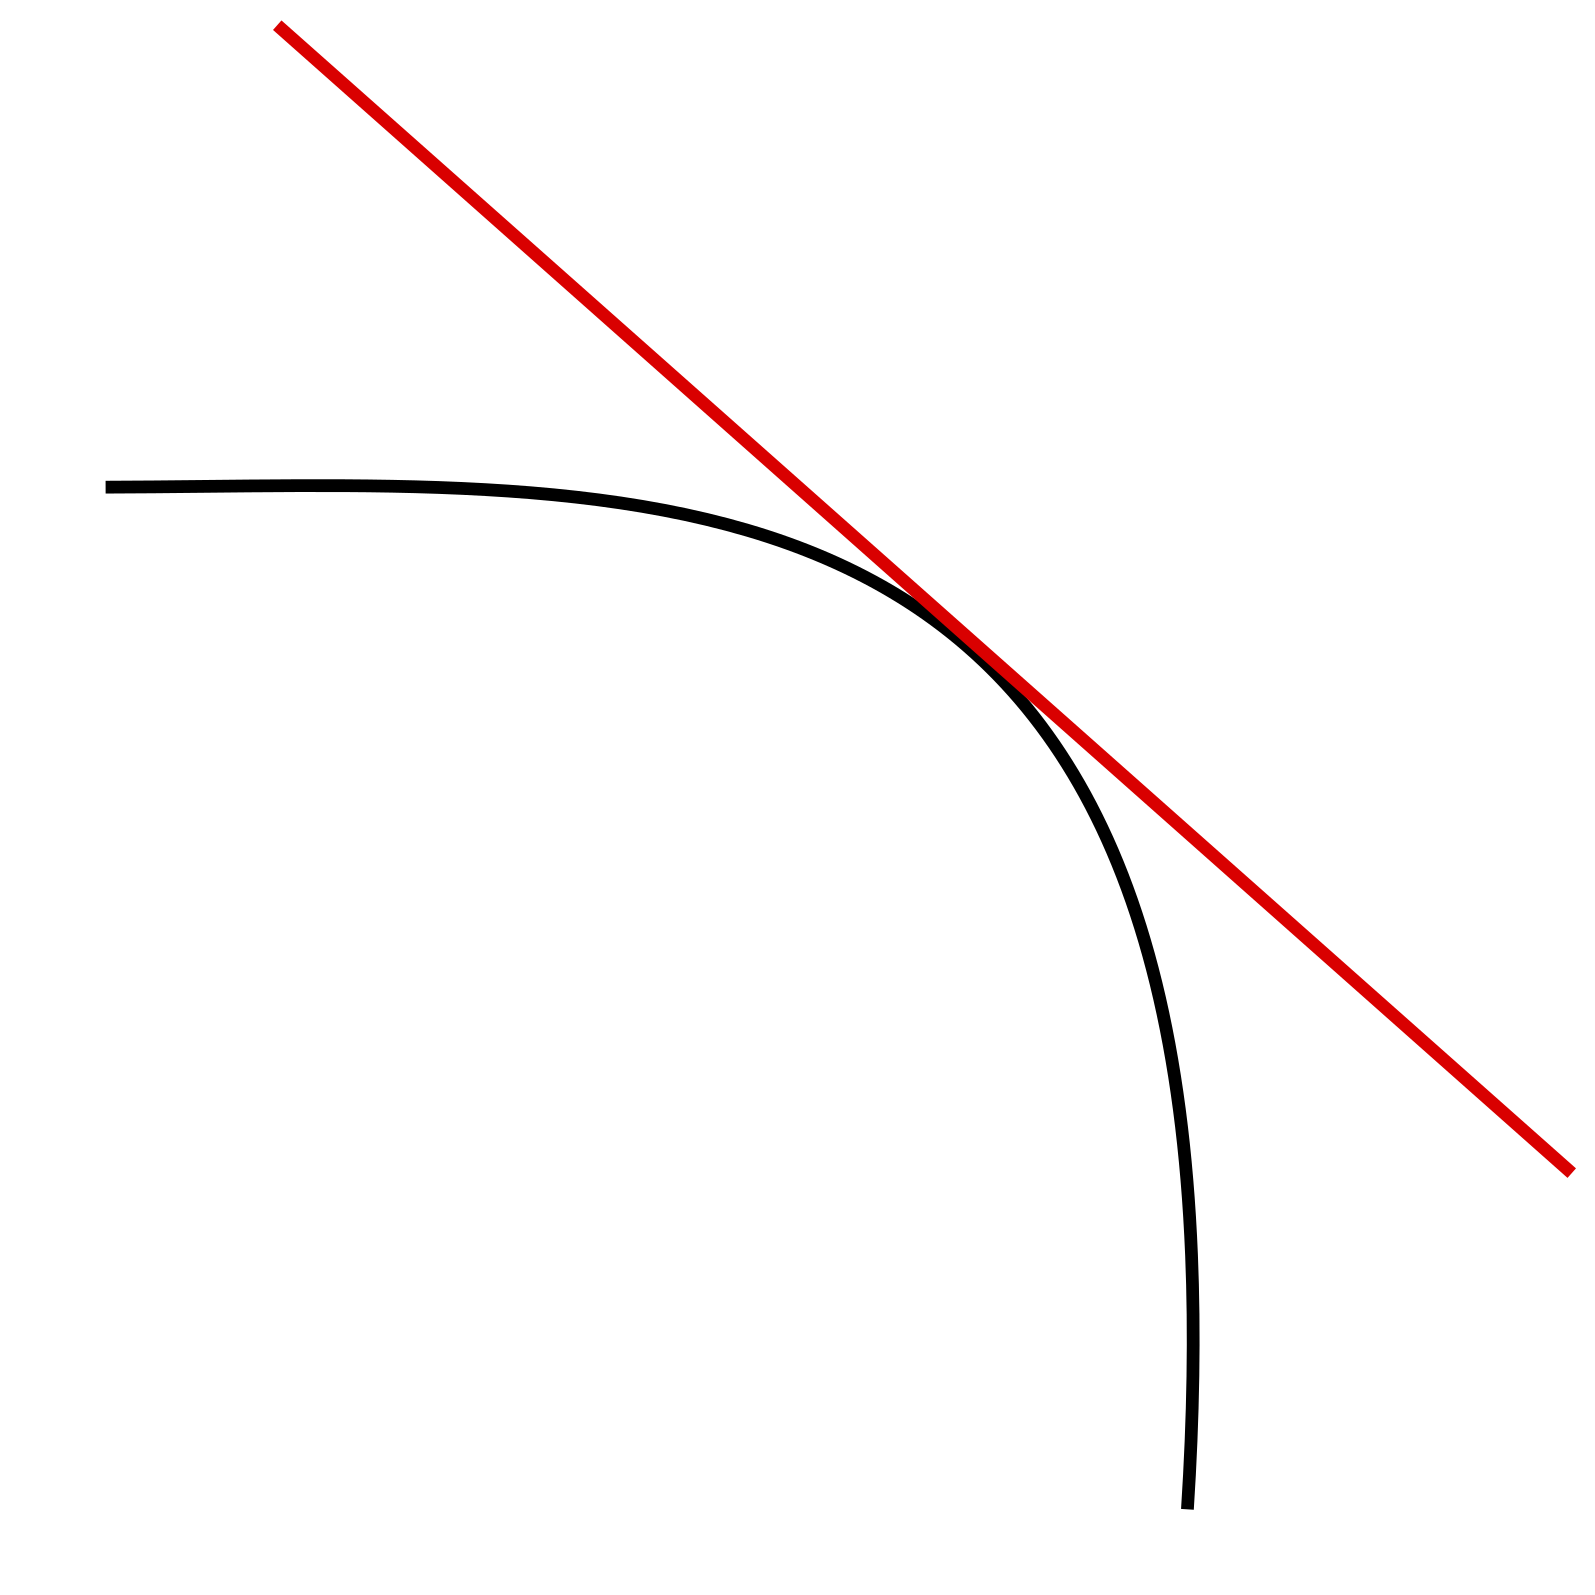
\includegraphics[width=0.9\linewidth, height=6cm]{convex.png}
        \caption*{Выпуклый график}
    \end{subfigure}
    \begin{subfigure}{0.5\textwidth}
        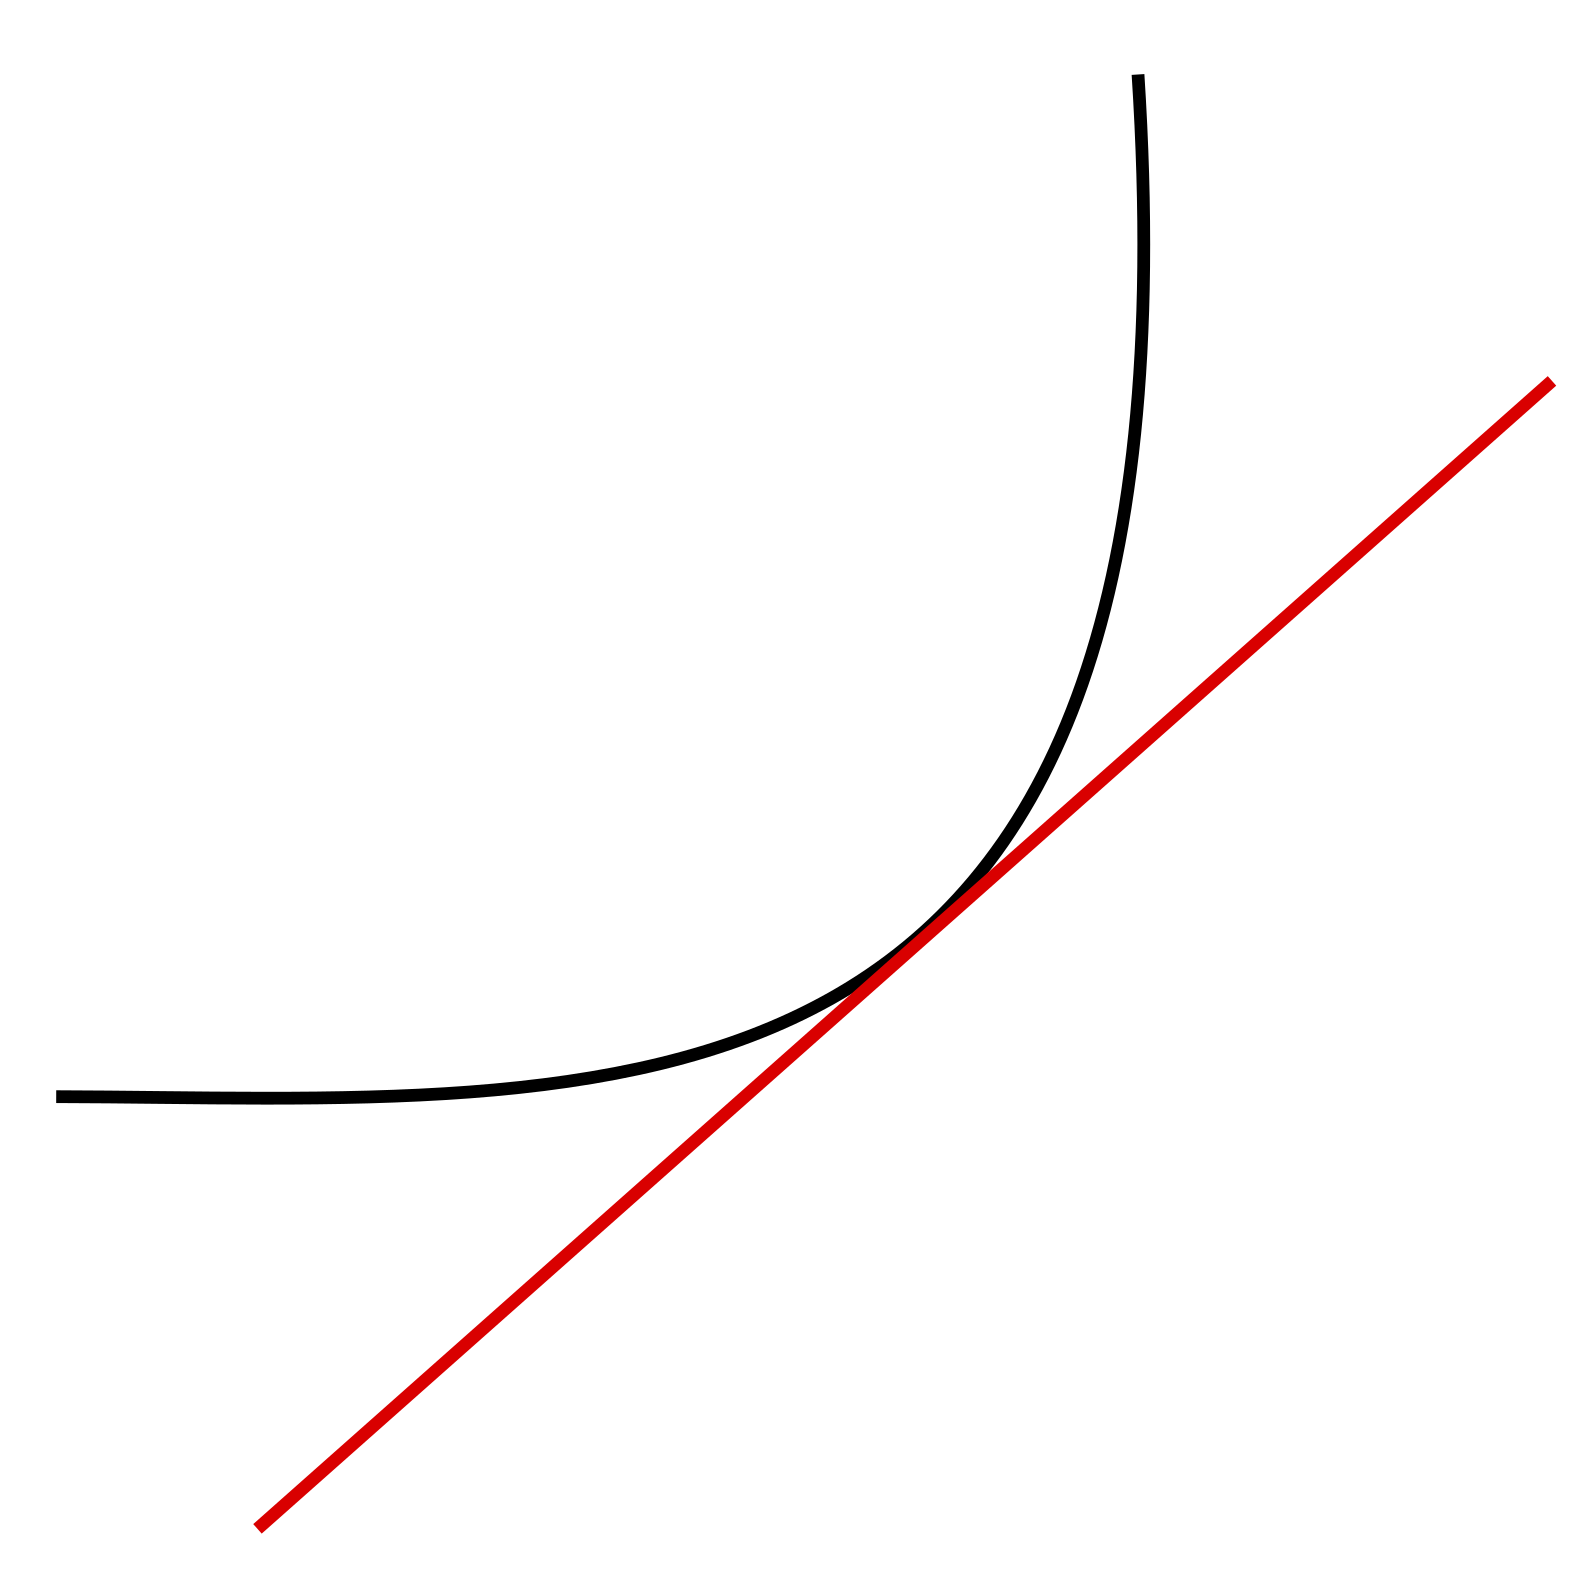
\includegraphics[width=0.9\linewidth, height=6cm]{concave.png}
        \caption*{Вогнутый график}
    \end{subfigure}
\end{figure*}

\section{Точки перегиба. Необходимое и достаточное условия перегиба}%
\label{sec:Точки перегиба. Необходимое и достаточное условия перегиба}

\begin{siderules}
    Пусть \(f(x)\) дифференцируема на \((a, b)\). Тогда точка \(M(x_0, f(x_0)), x_0 \in (a, b)\) называется \textbf{точкой перегиба}, если в данной точке существует касательная к графику функции и существует такая окрестность точки \(x_0\), в пределах которой график \(f(x)\) слева и справа от точки \(M\) имеет разные направления выпуклости.
\end{siderules}

\begin{theorem}[Достаточное условие вогнутости или выпуклости графика]
    \label{theorem:Достаточное условие вогнутости или выпуклости графика}
    \newpar
    Пусть \(f(x)\) определена на \((a, b)\). Кроме того \(\forall x \in (a, b) \; \exists f''(x)\). Тогда
    \begin{gather*}
        \forall x \in (a, b) \; f''(x) > 0 \implies \text{ кривая вогнутая} \\
        \forall x \in (a, b) \; f''(x) < 0 \implies \text{ кривая выпуклая}
    \end{gather*}
\end{theorem}

\begin{proof}
    Докажем случай при \(f''(x) < 0\). Доказательство для случая \(f''(x) > 0\) аналогичное.

    Пусть у нас есть две функции:
    \[
        \begin{cases}
            y = f(x)                                   \\
            y_{\text{кас}} = f(x_0) + f'(x_0)(x - x_0) \\
            x, x_0 \in (a, b)
        \end{cases}
    \]

    Кроме того, пусть \(x > x_0\). Случай при \(x < x_0\) рассмотрим позднее.

    Покажем, что график функции \(f(x)\) ниже касательной: для этого сравним ординаты в точке \(x\):
    \begin{gather*}
        y - y_{\text{кас}} = f(x) - (f(x_0) + f'(x_0)(x - x_0)) \\
        y - y_{\text{кас}} = f(x) - f(x_0) - f'(x_0)(x - x_0)
    \end{gather*}

    Поскольку \(f(x)\) определена и дифференцируема на \((a, b)\), воспользуемся \plink{theorem:Теорема Лагранжа}{теоремой Лагранжа}:
    \[
        f(x) - f(x_0) = f'(c)(x - x_0), c \in (x_0, x)
    \]

    Тогда
    \begin{gather*}
        y - y_{\text{кас}} = f'(c)(x - x_0) - f'(x_0)(x - x_0) \\
        y - y_{\text{кас}} = (x - x_0)(f'(c) - f'(x_0))
    \end{gather*}

    Снова воспользуемся \plink{theorem:Теорема Лагранжа}{теоремой Лагранжа}:
    \[
        f'(c) - f'(x_0) = f''(c_1)(c - x_0), c_1 \in (x_0, c)
    \]

    Тогда:
    \begin{gather*}
        \begin{cases}
            y - y_{\text{кас}} = f''(c_1)(c - x_0)(x - x_0) \\
            f''(c_1) < 0 \text{ (по условию)}               \\
            c - x_0 > 0                                     \\
            x - x_0 > 0
        \end{cases}
        \implies
        y < y_{\text{кас}}
    \end{gather*}

    Теперь рассмотрим случай, когда \(x < x_0\). Немного изменятся промежутки:
    \[
        \begin{cases}
            c \in (x, x_0) \\
            c_1 \in (x, c)
        \end{cases}
    \]

    Тогда:
    \begin{gather*}
        \begin{cases}
            y - y_{\text{кас}} = f''(c_1)(c - x_0)(x - x_0) \\
            f''(c_1) < 0 \text{ (по условию)}               \\
            c - x_0 < 0                                     \\
            x - x_0 < 0
        \end{cases}
        \implies
        y < y_{\text{кас}}
    \end{gather*}

    И при \(x > x_0\), и при \(x < x_0\) \(y < y_{\text{кас}}\) \(\forall x \in (a, b)\).
\end{proof}

\begin{theorem}[Необходимое условие существования точки перегиба]
    \newpar
    Если \(x_0\) — точка перегиба функции \(f(x)\) и данная функция имеет вторую производную в некоторой окрестности точки \(x_0\), причем в точке \(x_0\) она непрерывна, то \(f''(x) = 0\).
\end{theorem}

\begin{proof}
    Докажем от противного. Пусть \(f''(x_0) \neq 0\). Поскольку \(f(x)\) непрерывна при \(x = x_0\), то существует \(\delta\)-окрестность \(x_0\), в которой производная сохраняет свой знак, то есть:
    \[
        \forall x \in (x_0 - \delta, x_0 + \delta) \; f''(x_0) < 0
    \]

    В таком случае функция будет либо строго выпукла вверх (при \(f''(x) < 0\)), либо строго выпукла вниз (при \(f''(x) > 0\)). Но тогда точка \(x_0\) не является точкой перегиба. Это противоречие доказывает теорему.
\end{proof}

\begin{theorem}[Первое достаточное условие существования точки перегиба]
    \newpar
    Если функция \(f(x)\) непрерывна и дифференцируема в точке \(x_0\), имеет вторую производную \(f''(x)\) в некоторой проколотой \(\delta\)-окрестности точки \(x_0\) и вторая производная меняет знак при переходе через \(x_0\), то \(x_0\) является точкой перегиба функции \(f(x)\).
\end{theorem}

\begin{proof}
    Пусть вторая производная \(f''(x)\) при переходе через точку \(x_0\) меняет знак с плюса на минус. Тогда:
    \[
        \begin{cases}
            \forall x \in (x_0 - \delta, x_0) \; f''(x) > 0 \\
            \forall x \in (x_0, x_0 + \delta) \; f''(x) < 0
        \end{cases}
    \]

    В таком случае, согласно \plink{theorem:Достаточное условие вогнутости или выпуклости графика}{достаточному условию выпуклости}, функция \(f(x)\) выпукла вниз при \(x \in (x_0 - \delta, x_0)\) и выпукла вверх при \(x \in (x_0, x_0 + \delta)\). Следовательно в точке \(x_0\) функция меняет направление выпуклости, то есть по определению является точкой перегиба.
\end{proof}

\begin{theorem}[Второй достаточное условие существование точки перегиба]
    \newpar
    Пусть есть функция \(f(x): \exists f''(x_0) = 0\). Если \(\exists f'''(x) \neq 0\), то \(x_0\) является точкой перегиба функции \(f(x)\).
\end{theorem}

\begin{proof}
    Поскольку \(f'''(x_0) \neq 0\), то \(f''(x)\) либо строго возрастает (при \(f'''(x_0) > 0\)), либо строго убывает (при \(f'''(x_0) < 0\)). Так как \(f''(x) = 0\), то вторая производная имеет разные знаки в левой и правой \(\delta\)-окрестности точки \(x_0\). Отсюда, на основании предыдущей теоремы, следует, что \(x_0\) — точка перегиба функции \(f(x)\).
\end{proof}


\end{document}
